\chapter{2023 Luminosity Calibration}
\label{ch:2023_luminosity_calibration}

\section{Analysis of vdM data}

CMS's vdM scan program was performed in June 2023 during LHC fill 8999. During this fill, there were 138 filled bunches per beam and a total of 136 colliding bunches at the CMS IP. The bunches were designed to be wider than usual ($\beta^{*} = 1920 cm$) and separated by $525 ns$ in order to minimize afterglow effects. In order to minimize non-linear effects, the pileup was significantly limited from the average during 2023, $52$, to just $0.5$.

The LHC beam positions throughout the entire vdM program is shown in \autoref{fig:vdm_fill_program}.

\begin{figure}[!htb]
	\centering
	\makebox[\textwidth]{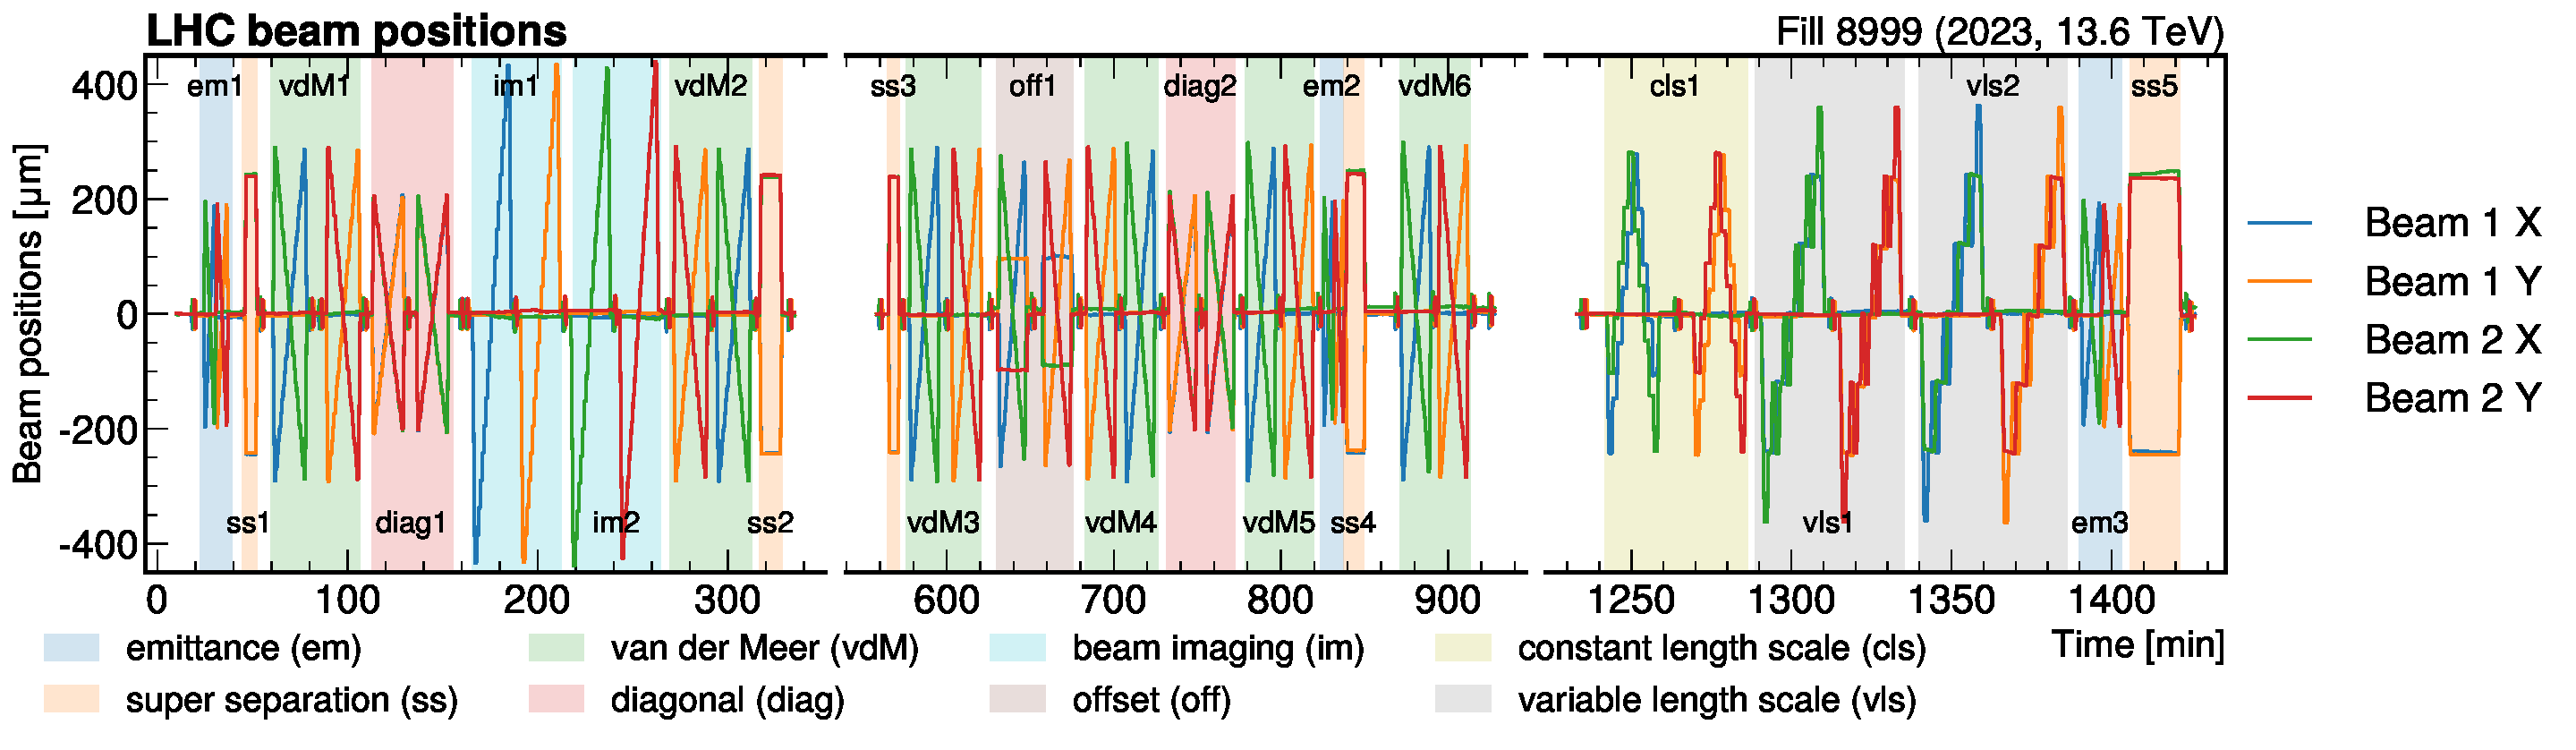
\includegraphics[width=0.95\paperwidth]{images/assets/vdm_fill_program.pdf}}
	\caption[Beam positions during fill 8999]{The vertical (X) and horizontal (Y) positions of beam 1 and beam 2 are shown as a function of time during LHC fill 8999 as measured by the LHC beam position monitors. Each kind of scan pair, which contains two orthogonal scans, is delimited by the shaded regions and labeled with the appropriate scan name. The cut out time periods correspond to when CMS was taking head-on data while the ATLAS vdM scan program was ongoing.}
	\label{fig:vdm_fill_program}
\end{figure}

As can be seen in \autoref{fig:vdm_fill_program}, during the vdM scans, the beams start by being maximally separated by approximately $578 \mu m$. They are then scanned across each other in 25 steps of approximately $48 \mu m$, remaining in the same position for 30 seconds for each step. In the beam imaging scans, one of the beams is fixed in the nominal head-on position while the other is moved from approximately $-433 \mu m$ to $+433 \mu m$ in 19 steps of 46 seconds each.

The measured luminometer rates are fitted as a function of the beam separation with the model described in \autoref{eq:double_gaussian_model} and the luminometer calibrations are determined from the fit parameters as detailed in \autoref{eq:calibration_from_fit_parameters}. The fits were performed on the data from the 6 vdM and the 2 im scan pairs and its associated cross-sections were measured. Figure \autoref{fig:no_Corr_xsec_results_HFET} shows the visible cross-section measurement results for the HFET luminometer with none of the corrections mentioned in \autoref{sec:experiment_conditions_and_corrective_procedures} having been applied.

\begin{figure}[!htb]
	\centering
	\makebox[\textwidth]{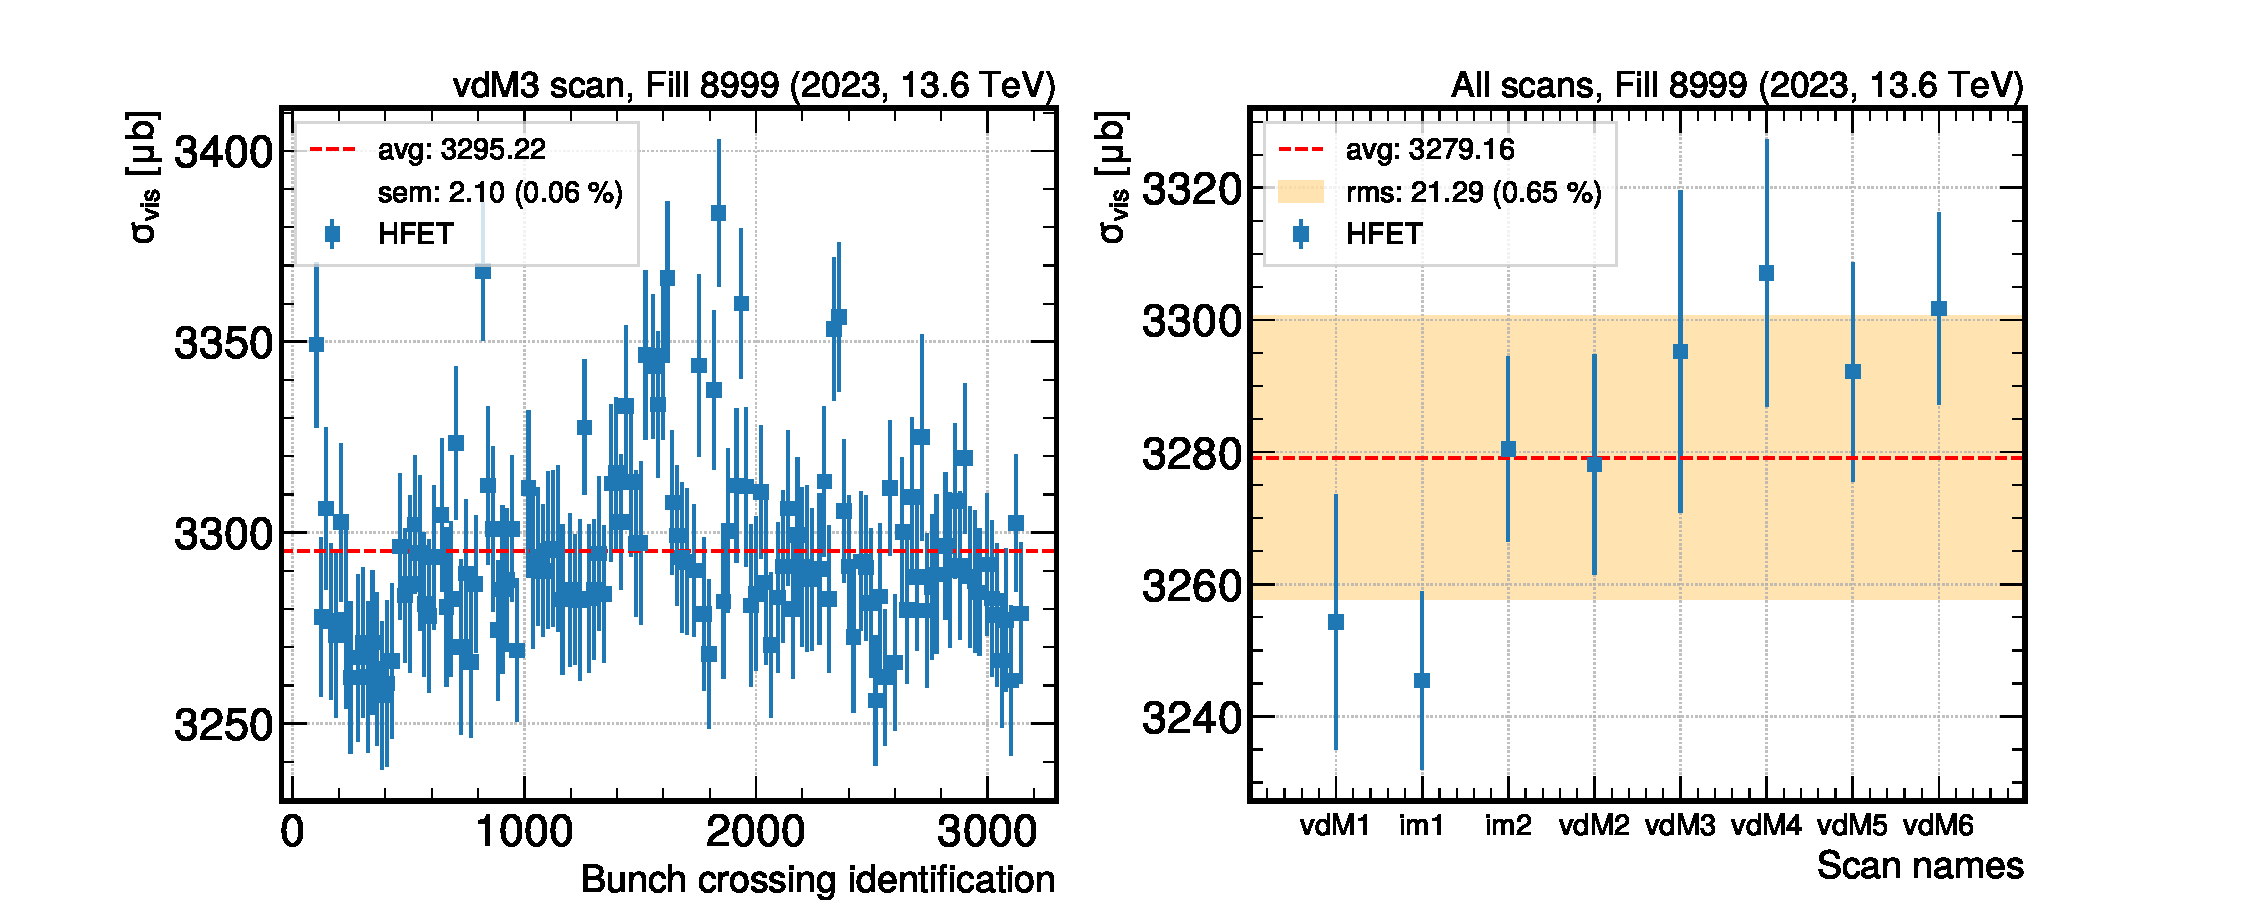
\includegraphics[width=0.9\paperwidth]{images/assets/no_Corr_xsec_results_HFET.pdf}}
	\caption[Initial HFET cross-section results]{Initial cross-section results obtained from uncorrected, raw data for the HFET luminometer, as an example. On the left, the measured per-bunch visible cross-sections with their associated fit uncertainties are shown. The standard error on the mean (sem) is also depicted in the legend. The right image shows the measured visible cross-section taking the average over all 136 BCIDs for each vdM and im scan pairs. The error bars are defined by the root mean squared (rms) over all BCIDs. The central value and its uncertainty are determined by calculating the uncertainty-weighted average and  standard deviation over the scan pairs.}
	\label{fig:no_Corr_xsec_results_HFET}
\end{figure}

There is a noticeable increasing trend in the measured visible cross-sections as a function of time. Furthermore, this trend is visible in all other luminometers, as can be seen in \autoref{fig:noCorr_luminometer_xsec}.

\begin{figure}[!htb]
	\centering
	\makebox[\textwidth]{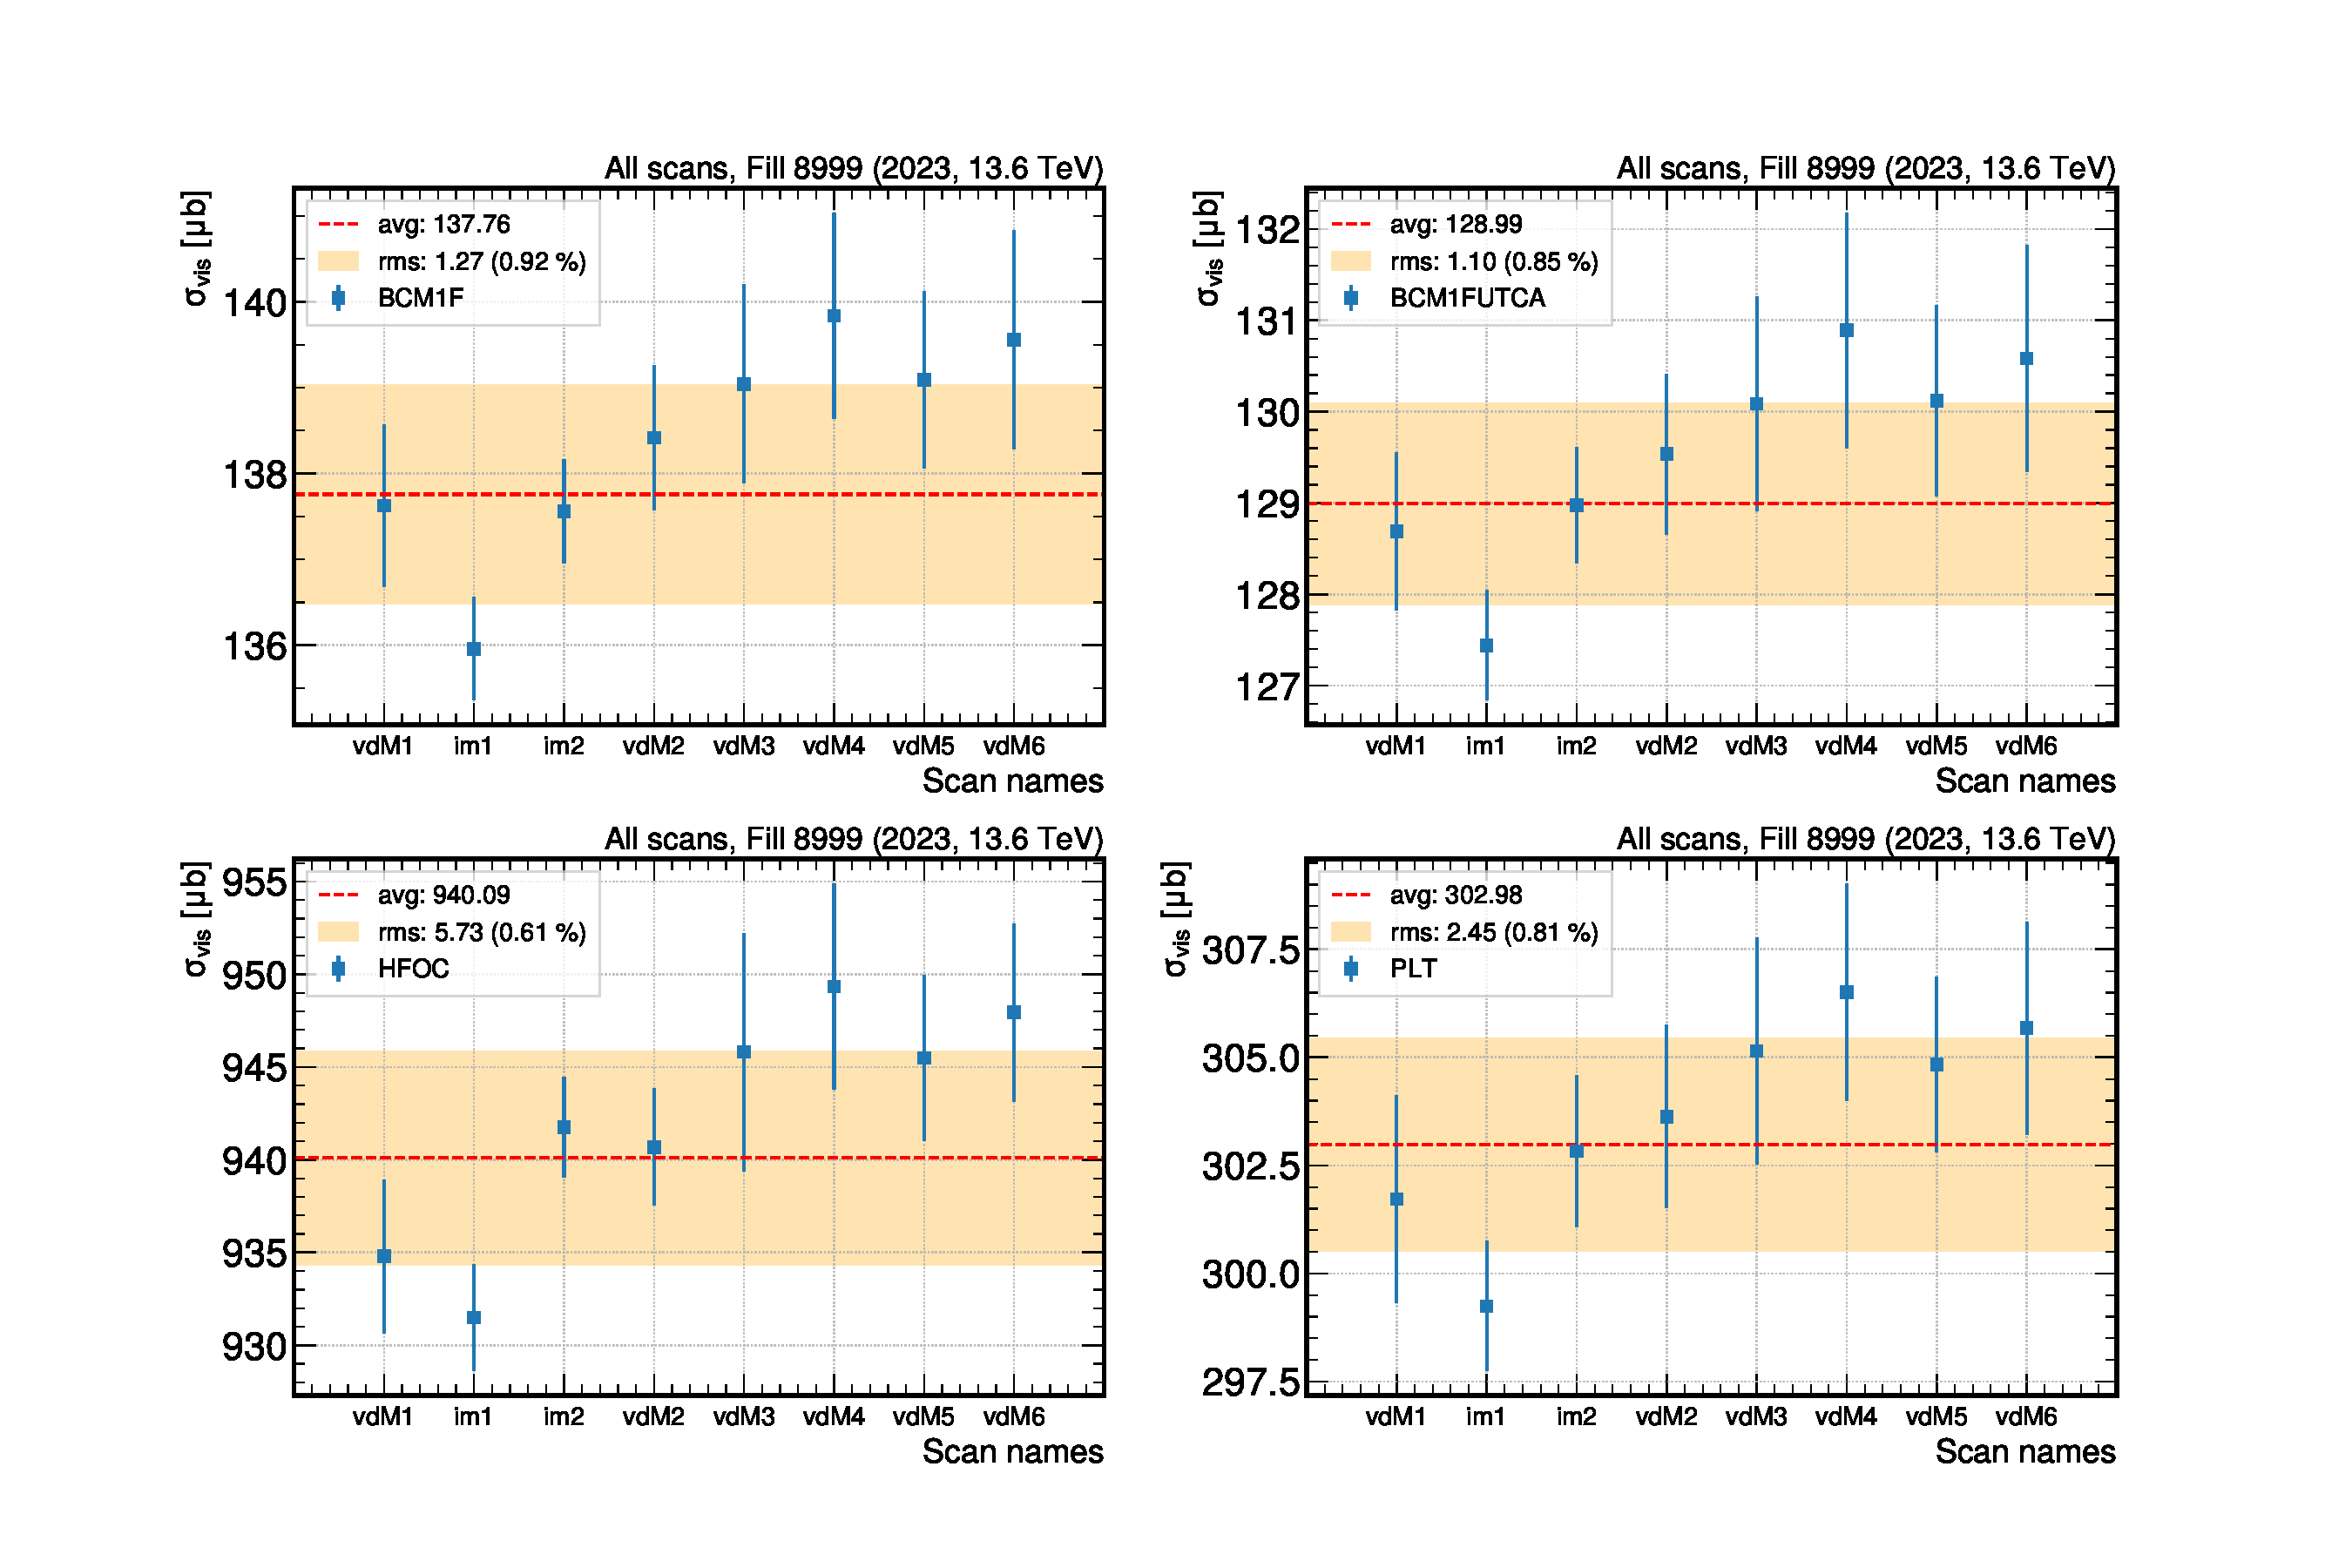
\includegraphics[width=0.9\paperwidth]{images/assets/noCorr_luminometer_xsec.pdf}}
	\caption[Initial cross-section for other online luminometers]{Initial cross-section results obtained from uncorrected, raw data for BCM1F, BCM1FUTCA, HFOC and PLT luminometers.}
	\label{fig:noCorr_luminometer_xsec}
\end{figure}

To increase the precision and accuracy of these measurements, a series of corrections have been applied to the raw data as will be described in the next subsections.

\subsection{Background estimation}

Beam-induced background and detector noise are both sources of background that are taken into account and subtracted from the raw detector rates. These sources have been estimated via two distinct methods:

\begin{itemize}
	\item \textbf{Estimation from super-separation scans}: The background contribution can be directly measured from super-separation scans (denoted as ss in \autoref{fig:vdm_fill_program}). During these scans, the beams are separated in both planes in order to render the contributions from collision products negligible. This method is most commonly used during special fills, such as the vdM fill, since it consumes beam time.
	\item \textbf{Estimation from non-colliding bunches}: An estimation for background can be done as long as there are filled but non-colliding bunches in the filling scheme. This indirect method assumes the background in colliding bunches can be described as:
	\begin{equation}
		\label{eq:bkg_eq1}
		\mathrm{BKG} = 2 \cdot \mathrm{BIB} + \eta
	\end{equation}
	where the beam-induced background, $\mathrm{BIB}$, from the two beams is considered as well as the detector-specific noise, $\eta$. Furthermore, $\mathrm{BIB}$ is calculated like:
	\begin{equation}
		\label{eq:bkg_eq2}
		\mathrm{BIB} = \mathrm{FNCR} + \eta.
	\end{equation}
	Here, $\mathrm{FNCR}$, is the measured rate from filled non-colliding bunches. Finally, the detector noise is calculated as the average signal from empty non-colliding bunches, $\mathrm{ENCR}$. Combining \autoref{eq:bkg_eq1} and \autoref{eq:bkg_eq2}, the background in colliding bunches is calculated as:
	\begin{equation}
		\mathrm{BKG} = 2 \cdot \mathrm{FNCR} + \mathrm{ENCR}.
	\end{equation}
	This method assumes the $\mathrm{BIB}$ contributions from both beams are the same, which may not be the case. Since super separation scans are never done under physics conditions, this method is the only option available for emittance scans during physics fills.
\end{itemize}

\autoref{fig:8999SuperSeparation_BCM1FUTCA} shows the BCM1FUTCA average of the measured rates for every BCID using the super-separation scan method. \autoref{tab:ss_summary} summarizes the measured background contributions for all the luminometers except for HFET since its background subtraction is applied online.

\begin{figure}[!htb]
	\centering
	\makebox[\textwidth]{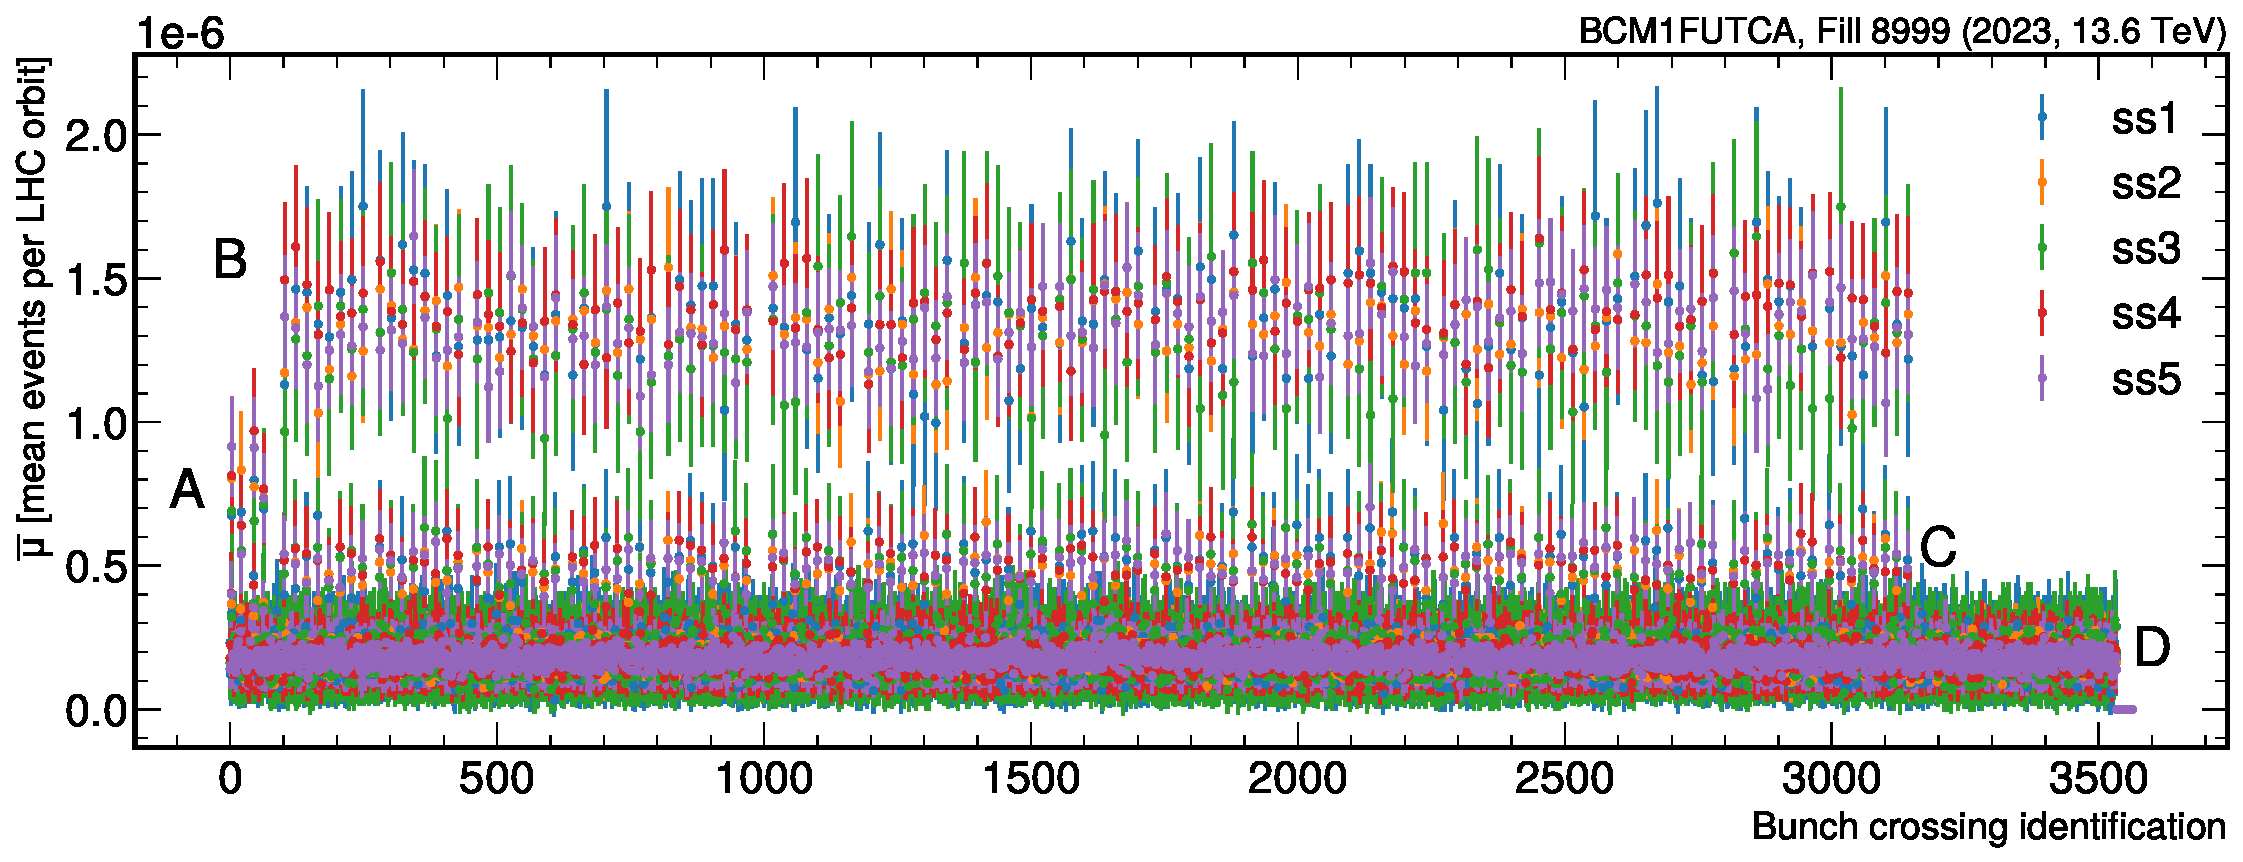
\includegraphics[width=0.8\paperwidth]{images/assets/8999SuperSeparation_BCM1FUTCA.pdf}}
	\caption[BCM1FUTCA hits in super-separation scan]{BCM1FUTCA average of the measured rates per BCID during super separation scans. The labels A, B, C, and D refer to the following: A represents the four filled non-colliding BCIDs at the beginning of the orbit, B represents the 136 colliding BCIDs (indicated by the top band), C corresponds to the empty BCIDs adjacent to filled BCIDs (around 0.5), and D represents the remaining empty non-colliding bunches.}
	\label{fig:8999SuperSeparation_BCM1FUTCA}
\end{figure}

\begin{table}[!htb]
	\centering
	\caption[Background impact on calibration]{Summary of measured background per luminometer and its impact on the vdM calibration. The average is computed on the measured background for all the colliding bunches across all scans. The associated uncertainty is the standard error on the average.}
	\begin{tabular}{lcccc}
		\hline
		Luminometer & Average [$\overline{\mu}$] & Uncertainty [$\overline{\mu}$] & \% to peak rate at vdM1 & Effect on $\sigma_{\mathrm{vis}}$ (\%) \\
		\hline
		BCM1F & 1.59E-6 & 4.68E-9 & 0.18 & -1.56 \\
		BCM1FUTCA & 1.34E-6 & 4.63E-9 & 0.16 & -1.39 \\
		HFOC & 1.17E-7 & 6.10E-9 & 0.002 & -0.02 \\
		PLT & 2.11E-6 & 9.25E-9 & 0.11 & -1.05 \\
		PCC & 1.65E-2 & 6E-4 & 0.12 & -1.08 \\
		\hline
	\end{tabular}
	\label{tab:ss_summary}
\end{table}

\subsection{Beam current measurement}
\label{subsec:beam_current_measurement}

The beam currents play a crucial role in the determination of the visible cross-section, serving as a normalization factor to the detector rates, as can be seen from \autoref{eq:calibration_from_fit_parameters}. In the LHC, they are measured with two dedicated instruments: the Fast Beam Current Transformer (FBCT) \cite{Belohrad:1267400} and the Direct-Current Current Transformer (DCCT) \cite{Odier:1183400}.

\begin{figure}[!htb]
	\centering
	\makebox[\textwidth]{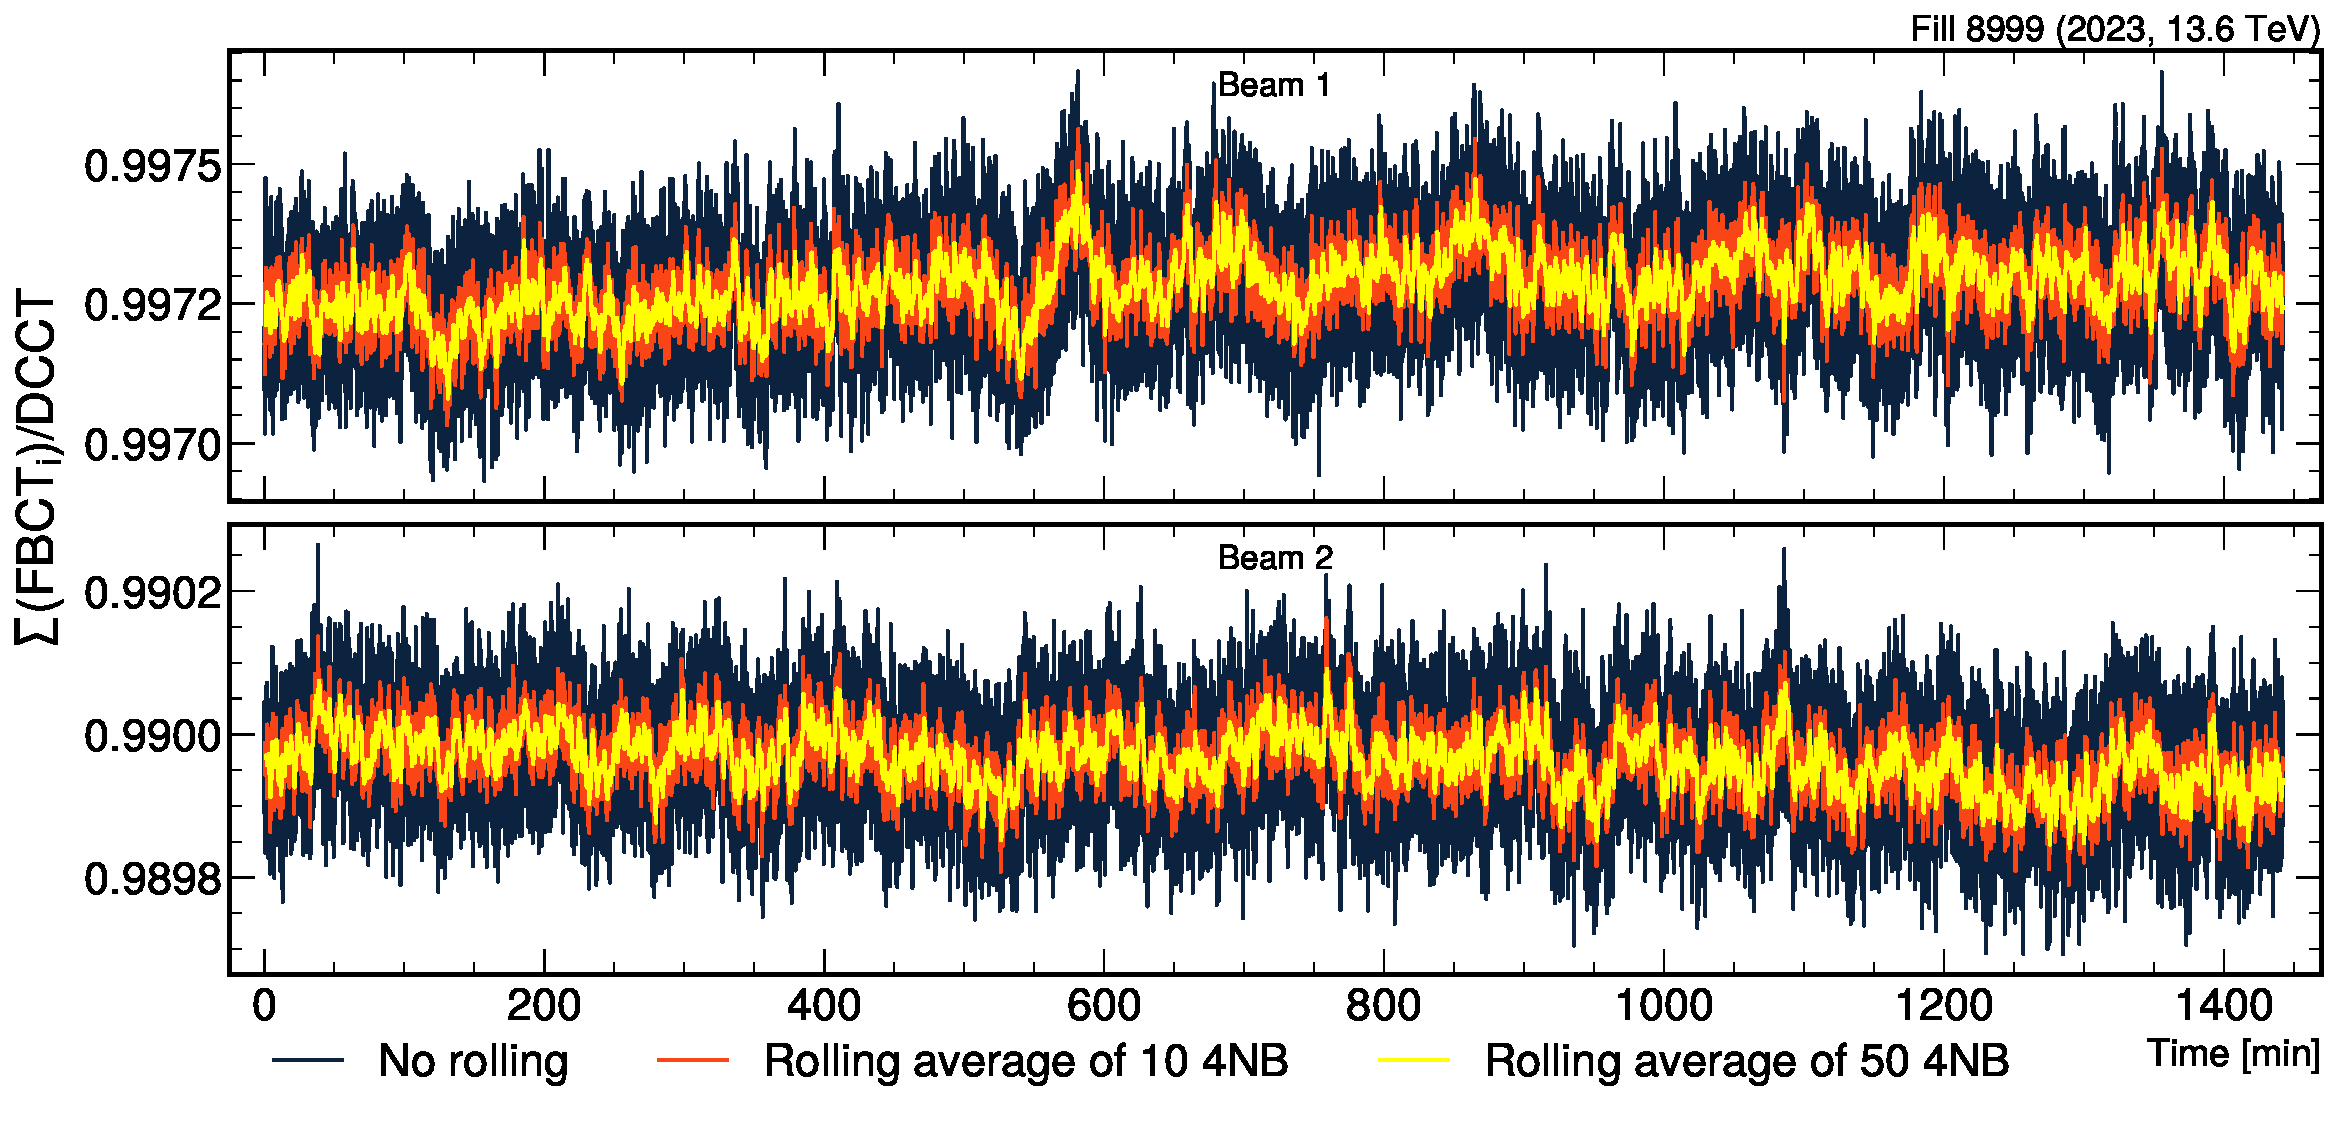
\includegraphics[width=0.8\paperwidth]{images/assets/fbct_dcct_calibration.pdf}}
	\caption[FBCT to DCCT calibration]{Value of the FBCT to DCCT calibration throught the vdM fill 8999. The calibration factor is computed as the ratio between the orbit-integrated FBCT measurements and that of DCCT.}
	\label{fig:fbct_dcct_calibration}
\end{figure}

The FBCT system is able to provide current measurements with per-bunch granularity (every 25ns) while DCCT provides orbit integrated measurements with an associated uncertainty of 0.2\% \cite{Barschel:2649533}, achieving higher levels of accuracy compared to FBCT \cite{Gras:1379466}. This motivates a calibration procedure in which the orbit-integrated FBCT measurements are normalized to the measurements from DCCT. \autoref{fig:fbct_dcct_calibration} shows the value of this calibration across the entire vdM fill for both beams.

The application of this correction is done only in the measurements that correspond to time intervals where a scan is being performed. The overall magnitude of this calibration is calculated as the average among all the scan steps. \autoref{fig:fbct_dcct_vdM1_calibration} shows the calibration used for the first vdM scan pair, vdM1.

\begin{figure}[!htb]
	\centering
	\makebox[\textwidth]{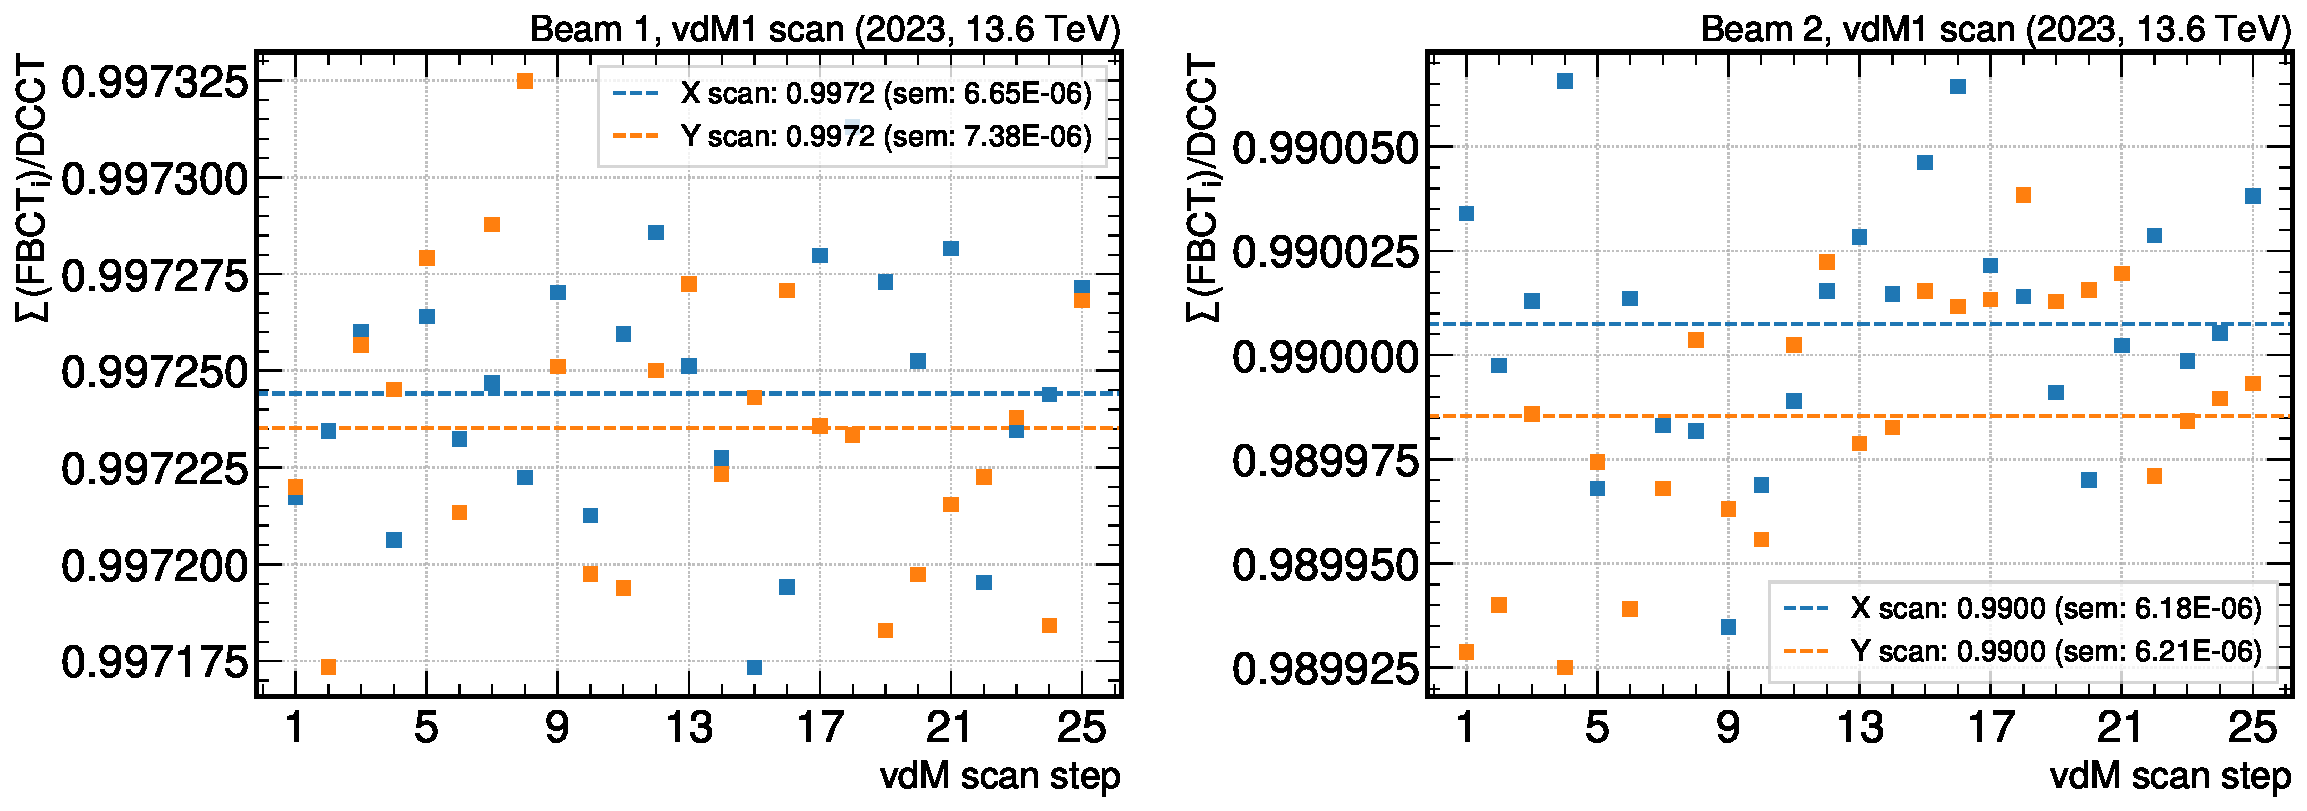
\includegraphics[width=0.8\paperwidth]{images/assets/fbct_dcct_vdM1_calibration.pdf}}
	\caption[FBCT calibration for scan pairs]{Calculated FBCT to DCCT calibration for the scan pairs of the first vdM scan in fill 8999. Every squared point corresponds to the ratio between the orbit-integrated FBCT beam current and the measurement from DCCT for a given scan step (25 in total for a vdM scan). The average and error on the mean are shown in the legend.}
	\label{fig:fbct_dcct_vdM1_calibration}
\end{figure}

Both systems are also susceptible to the presence of erratic charges. As mentioned in \autoref{subsec:particle_beams_lhc} only one out of the 10 RF buckets in a bunch crossing are nominally filled. Spurious charges in the nominally empty buckets, referred to as ``ghost charges", have an impact on the DCCT measurements but do not have an effect on the per-bunch FBCT measurement, since it is impervious to charges below a given threshold. Another class of additional charges, called ``satellites", emerge in the RF buckets adjacent to the nominally filled one. These extra charges affect the FBCT measurements. \autoref{fig:ghost_satellite_illustration} illustrates the position of these charges in relation to the main bunch. 

\begin{figure}[!htb]
	\centering
	\makebox[\textwidth]{\includegraphics[width=0.6\paperwidth]{images/assets/ghost_satellite_illustration.png}}
	\caption[Longitudinal bunch profile with LDM]{Longitudinal profile taken with the LDM, in logarithmic scale. The ghost charges are evenly spread while the satellites are adjacent to the main bunch (from \textit{Ref.} \cite{Alici:1427728}).}
	\label{fig:ghost_satellite_illustration}
\end{figure}

The LHC Longitudinal Density Monitor (LDM) system, measures the fraction of ghost charges in the DCCT measurement, $f_{ghost}$, as well as the per-bunch satellite fractions in the FBCT measurements, $f_{sat_i}$. Combining the calibration procedure specified above with the corrections from these LDM measurements, the total correction to the beam current can be expressed as:
\begin{equation}
	n_{i} = \frac{\mathrm{FBCT}_i \left( 1 - f_{sat_i} \right) \cdot \mathrm{DCCT} \left( 1 - f_{ghost} \right)}{\sum_i \mathrm{FBCT}_i}
\end{equation}
where $n_{i}$ is the corrected current for BCID $i$.

These corrections have a similar effect on all luminometers. The FBCT to DCCT calibration decreased the visible cross-section by 1.27\% with an associated uncertainty equal to that of the DCCT measurement, 0.2\%. The correction from ghost-satellite charges had a +0.1\% effect on the detector calibration and the full correction was taken as an uncertainty.

\subsection{Length scale calibration}

During a vdM scan pair, the beams perform 25 steps in both planes. The movement of these beams is controlled with a pair of steering dipoles located on either side of the IP. However, the scale of each step may differ from the nominally intended step length. For example, an intended nominal step of, say, 1 $\mu m$ may correspond to $0.99$ $\mu m$. This can be generalized for any nominal position, $x_{\mathrm{nom}}$, and the associated actual measurement, $x_{\mathrm{real}}$, as:
\begin{equation}
	x_{\mathrm{meas}} = \alpha x_{\mathrm{nom}}
\end{equation}
where $\alpha$ is called the length scale factor. This parameter encodes the first-order linear response of the magnets to the nominal input positions.

This correction revolves around the comparison between the nominal and actual beam spot positions. The beam spot is the overall distribution of the vertices reconstructed from tracks registered in the tracking detector and its position refers to the average of this position. The CMS tracker \cite{Sirunyan:2759951}, provides the actual beam spot measurements, $\overline{x^{\mathrm{real}}_{\mathrm{BS}}}$, and the nominal measurement assumes that the individual beam profiles are Gaussian and factorizable. Therefore, the beam spot is computed as the weighted average from the two beams as \cite{CMS-PAS-LUM-22-001}:
\begin{equation}
	\overline{x^{\mathrm{nom}}_{\mathrm{BS}}} = \frac{\overline{x_1}\sigma_{x1}^{-2} + \overline{x_2}\sigma_{x2}^{-2}}{\sigma_{x1}^{-2} + \sigma_{x2}^{-2}},
\end{equation}
and similarly for the y direction. The $\overline{x^{\mathrm{nom}}_{\mathrm{BS}}}$ is the nominal beam spot position and $\overline{x_1}$ and $\overline{x_2}$ are the means of the beam profiles.

In practice, the length scale scans, as shown in \autoref{fig:vdm_fill_program}, are used. There are two versions of these scans: constant length scale (cls) scans and variable length scale (vls) scans. The cls scans are made up of 2 stages: forward stage, when the beams are moved from negative to positive positions, and the backward stage, where the beams are moved from positive to negative positions. In the cls scan, the relative beam separations are kept constant. In the vls scans, we have a cycle repeating a total of five times. This cycle comprises the moments in which beam 1 is above beam 2 (Up), the beams are head-on and, lastly, when beam 1 is below beam 2 (Dn). \autoref{fig:length_scale_scans} shows the beam positions during the cls1 and vls1 scan pairs.

\begin{figure}[!htb]
	\centering
	\makebox[\textwidth]{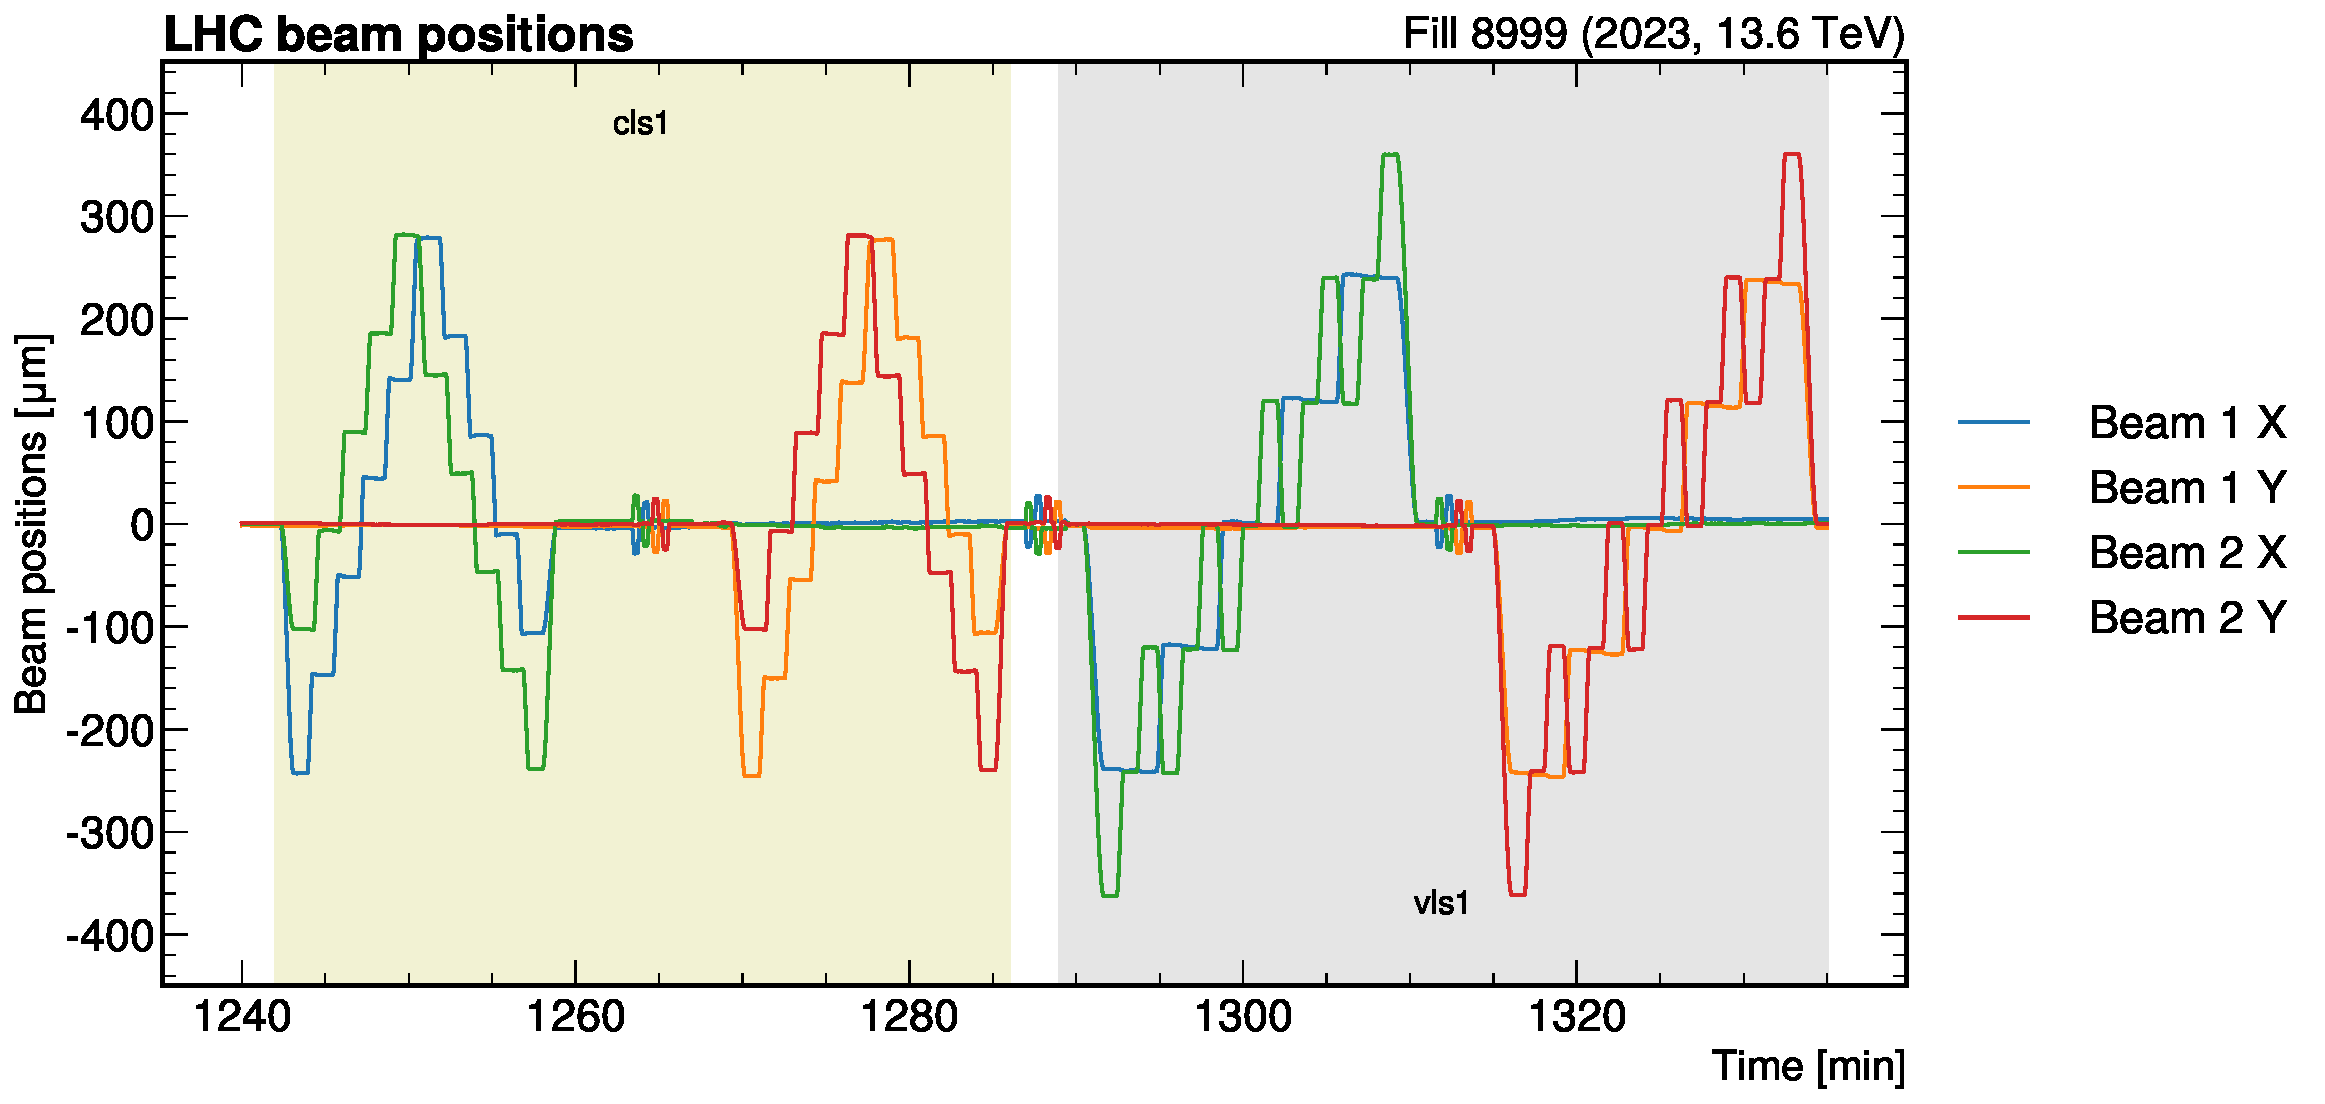
\includegraphics[width=0.6\paperwidth]{images/assets/length_scale_scans.pdf}}
	\caption[Beam positions in length scale scans]{Beam positions during the constant and variable length scale scans.}
	\label{fig:length_scale_scans}
\end{figure}

The difference between the real and nominal beam spot measurements are plotted as a function of the beam positions and a linear fit is performed to obtain the $\alpha$ factor. An example fit for the Up stage of the variable length scale scan is shown in \autoref{fig:fig:variable_length_scale_fit}. The overall length scale factor was calculated from a weighted average on the factors obtained from every possible scan and scan stage. The results are summarised in \autoref{fig:length_scale_fit_summary}.

\begin{figure}[!htb]
	\centering
	\makebox[\textwidth]{\includegraphics[width=0.4\paperwidth]{images/assets/variable_length_scale_fit.png}}
	\caption[Length scale factor determination]{Determination of the length scale factor $\alpha$ from a variable length scale scan (from \textit{Ref.} \cite{CMS-DP-2024-068}).}
	\label{fig:fig:variable_length_scale_fit}
\end{figure}

As the backward stage of the constant length scale for the vertical plane yielded poor quality fit results, it was not included in the weighted average. However, in order to account for this in the associated uncertainty, a systematic uncertainty was added to the already-obtained $0.0011$ rms. This systematic was computed as the difference between the weighted average with and without this faulty scan stage and has an absolute value of $0.0012$. This results in a total uncertainty for the length scale factor in the y plane of $\sqrt{0.0011^2 + 0.0012^2} \approx 0.0016$.

The final uncertainty is the quadrature sum of the uncertainties in both planes, 0.2\%. The effect of this correction impacts all luminometers equally and resulted in a a decrease of the $\sigma_{\mathrm{vis}}$ of $0.9\%$.

\begin{figure}[h!]
	\centering
	\makebox[\textwidth]{\includegraphics[width=0.7\paperwidth]{images/assets/length_scale_fit_summary.png}}
	\caption[Length scale calibration results]{Results of the length scale calibration for the X (left) and Y (right) coordinates, using constant-separation length scale (cls) scans in the forward (fwd) and backward (bkw) directions, and variable-separation length scale (vls) scans (analysed as cls scans) for beam 1(2) scan with beam 2(1) (b2(b1)) being separated in the direction down (Dn) or up (Up) (from \textit{Ref.} \cite{CMS-DP-2024-068}). Length scale values are shown for fits whose reduced-$\chi^2$ is below 100, which was not the case for cls bkw scan in the Y plane.}
	\label{fig:length_scale_fit_summary}
\end{figure}

\subsection{Beam-beam effects}

When proton bunches collide at the IP, a repulsion force will be felt due to their electromagnetic interaction. This interaction will have an effect on the luminomenter rates, on the beam separations and, consequently, on the measured visible cross-section. These effects, referred to as beam-beam effects, are corrected for in 2 ways.

As a product of the repulsive forces, the beam orbits will be deflected. The tranverse electric field felt due the interaction of the 2 particle bunches, $E(x, y)$, is calculated using the Bassetti-Erskine formula \cite{Bassetti:122227}. With the knowledge of the tranverse electric field, the deflection angle caused by electrostatical repulsion and the orbit shifts can be calculated with \autoref{eq:beam_deflection_angle} and \autoref{eq:beam_orbit_deflection} \cite{PhysRevLett.62.2949}, respectively.

\begin{equation}
	\theta_{\chi} = \frac{2r_p}{\gamma} N_p E_{\chi}(x, y), \, \mathrm{with} \, \chi \in \{ x, y \}
	\label{eq:beam_deflection_angle}
\end{equation}

\begin{equation}
	\delta_{\chi} = \frac{\theta_{\chi} \beta^{*}}{2 \mathrm{tan} \left( \pi Q_{\chi} \right)}, \, \mathrm{with} \, \chi \in \{ x, y \}
	\label{eq:beam_orbit_deflection}
\end{equation}

In these equations, $r_p$ is the classical proton radius, $N_p$ is the opposing bunch population, $\gamma$ is the relativistic factor for proton and $Q_{\chi}$ is the betatron tune, a beam optics parameter specific to the each experiment. The calculated orbit deflections, $\delta_{\chi}$, are then used to correct the nominal beam separations for every bunch crossing and at each scan step.

When the bunches cross each other, the shape of the convoluted bunch distributions will also be affected by the electromagnetic interaction. This effect, commonly called dynamic-$\beta$ effect, is the second beam-beam effect that is taken into account. The distorted beam overlap shape will be reflected in a $\beta^{*}$ value different from the nominal one, which will effect the measured rates. This way, a corrective factor is multiplied to the measured rates in order to account for this effect.

The magnitude of both corrections, beam-beam deflection and dynamic-$\beta$, are shown in \autoref{fig:beam_effects_correcions}.

\begin{figure}[!htb]
	\centering
	\makebox[\textwidth]{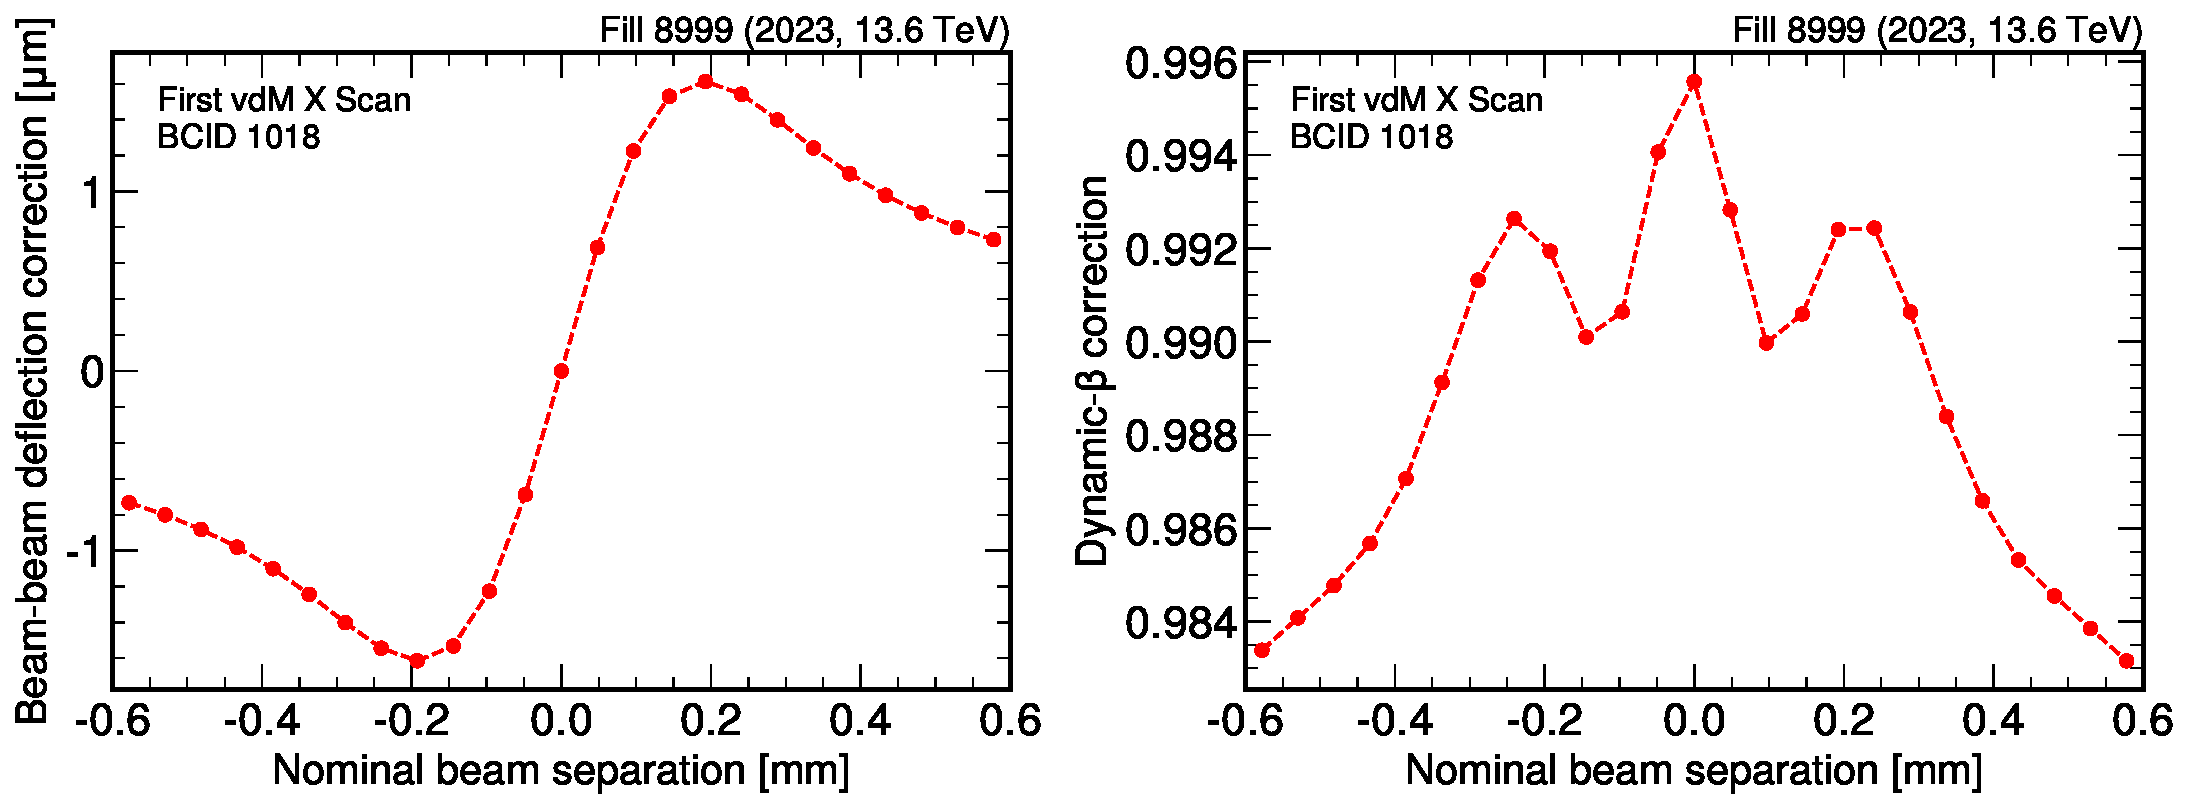
\includegraphics[width=0.7\paperwidth]{images/assets/beam_effects_correcions.pdf}}
	\caption[Electromagnetic interaction correction]{Correction values for the electromagnetic interaction between the 2 bunches. On the left, the orbit deflections due to electromagnetic repulsion are shown while on the right, the rate correction factors due to the distortion of the beam overlap shape are depicted.}
	\label{fig:beam_effects_correcions}
\end{figure}

Applying these corrections to all vdM and im scans yields an increase in $\sigma_{\mathrm{vis}}$ of 0.7\% for all luminometers. The associated uncertainty is computed from the quadrature sum of all the relevant sources of uncertainty summarised in \autoref{tb:beam_beam_uncertainty_summary}. A more detailed explanation of the beam-effects, the corrections and their associated uncertainties can be found in \cite{babaev2021coherentdeflectionellipticbunches}.

\begin{table}
	\centering
	\caption[Beam-beam systematic uncertainty]{Contributions to total beam-beam systematic uncertainty. Detailed description of these sources can be found in \cite{babaev2021coherentdeflectionellipticbunches}}\label{tab:bb:1}
	\label{tb:beam_beam_uncertainty_summary}
	\begin{tabular}{l|c}
		\hline
		Source & Uncertainty (\%) \\
		\hline
		Nominal tunes & 0.15 \\
		$\beta^{*}$ at IP5 & 0.11 \\
		Non-Gaussian tails & 0.16 \\
		Beam size imbalance & 0.01 \\
		Reference ambiguity & 0.20 \\
		Multi-IP tune shift & 0.04 \\
		Ellipticity & 0.03 \\
		Polynomial & 0.10 \\
		\hline
		Total & 0.34 \\
		\hline
	\end{tabular}
\end{table}

\subsection{Orbit drift}

Any drift in the beam positions, be it random or systematic, will result in a discrepancy from the nominal positions and, consequently, affect the visible cross-section measurements. To correct for this effect, 2 beam position monitor systems (BPM) are used: the Diode Orbit and Oscillation System (DOROS) \cite{Gąsior:2313935} and the BPMs located in the LHC arcs (arcBPM) \cite{Sirunyan:2759951}.

The correction applied to the nominal beam positions, using the measurements from both BPMs, is done in 2 steps.

\begin{itemize}
	\item \textbf{Linear orbit drift}: In this correction, BPM measurements that are taken immediatly before and after the scans, when the beam are in their nominal head-on positions, are used to determine the linear orbit drift at each step of a scan. To this effect, a linear interpolation is performed between these 2 points, for every scan, and the nominal positions are corrected accordingly. \autoref{fig:linear_orbit_drift_vdm1x} shows this procedure applied to the first vdM scan done in the horizontal transverse direction and \autoref{fig:linear_orbit_drift_correction} illustrates the orbit drift for all vdM and im scan pairs.

	\begin{figure}[!htb]
		\centering
		\makebox[\textwidth]{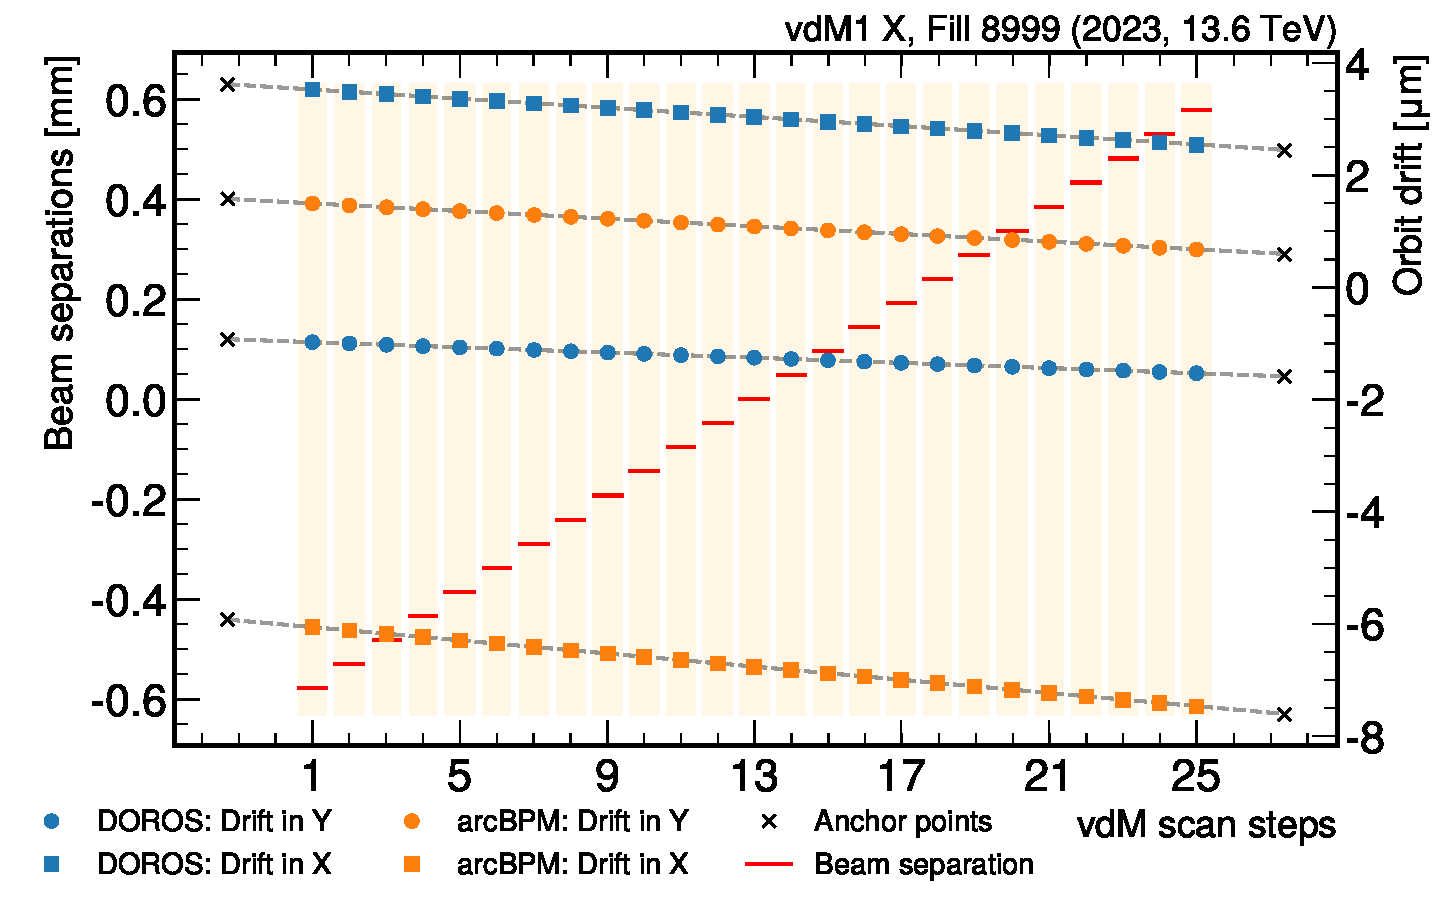
\includegraphics[width=0.6\paperwidth]{images/assets/linear_orbit_drift_vdm1x.pdf}}
		\caption[Orbit drift correction calculation]{Orbit drift correction calculated from the interpolation of the BPM measurements done before and after the vdM1 scan in the horizontal plane. The nominal beam separations (left axis), at every scan step and in $mm$,  are represented by the solid red lines, the interpolated points can be seen as black crosses. The linear interpolation was conducted for both BPM systems, DOROS (blue) and arcBPM (orange), and both planes, horizontal (squares) and vertical (circles). The orbit drifts (right axis) are expressed in $\mu m$.}
		\label{fig:linear_orbit_drift_vdm1x}
	\end{figure}

	\begin{figure}[!htb]
		\centering
		\makebox[\textwidth]{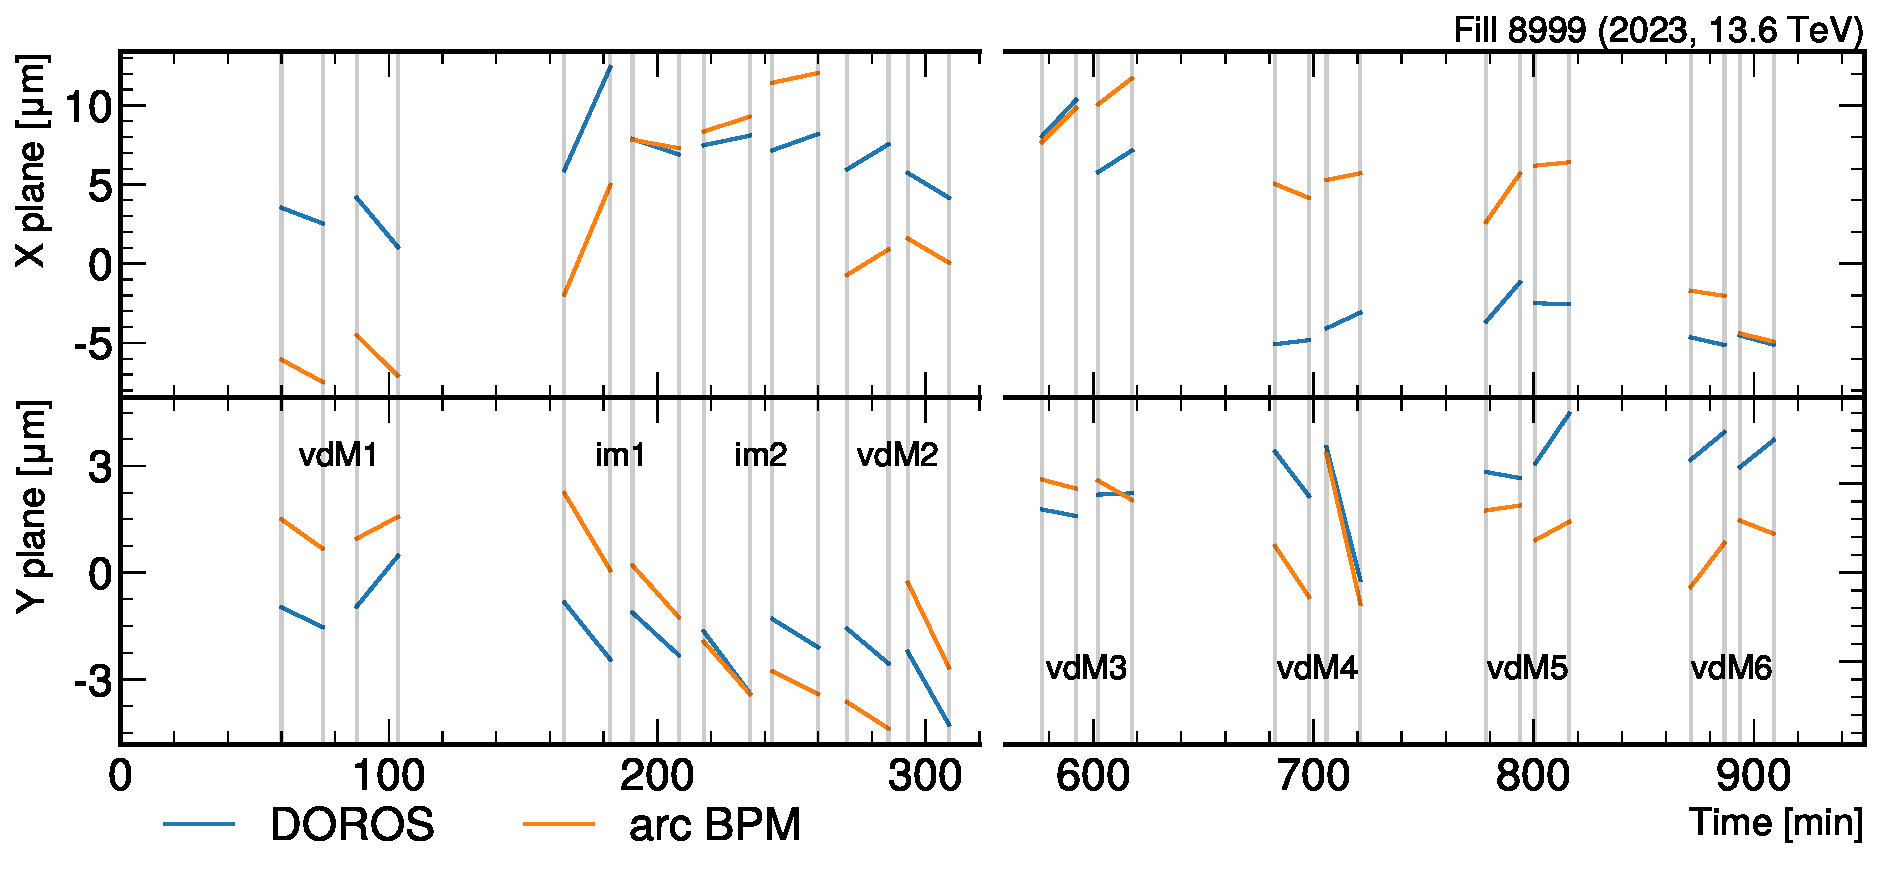
\includegraphics[width=0.8\paperwidth]{images/assets/linear_orbit_drift_correction.pdf}}
		\caption[Orbit drift correction summary]{Orbit drift correction for all vdM and im scan pairs.}
		\label{fig:linear_orbit_drift_correction}
	\end{figure}

	After correcting for the orbit drift in the nominal beam separations, we follow up with a correction to the measured rates in the non-scanning direction. To understand why, let us recall our assumption that the particle bunch distributions are XY-factorizable. Under this assumption, the rates measured in some arbitraty $(x, y)$ point would be:
	\begin{equation}
		R\left( x, y \right) = r_x(x) \cdot r_y(y).
	\end{equation}
	Taking the vertical plane as non-scanning, for example, an orbit drift ($\Delta_y$) would mean that our measured rates would be given as:
	\begin{equation}
		R\left( x, y + \Delta_y \right) = r_x(x) \cdot r_y(y + \Delta_y).
	\end{equation}
	We can then combine the 2 equations to arrive at the rate correction:
	\begin{equation}
		R\left( x, y\right) = R\left( x, y + \Delta_y \right) \cdot \frac{r_y(y)}{r_y(y + \Delta_y)}.
	\end{equation}

	\item \textbf{Residual orbit drift}: After the linear orbit drift correction is applied there remain some residual differences between the nominal and the BPM measured beam positions. The length scale and the beam-beam deflection corrections are part of this residual difference and are accounted for as described in the previous sections. To correct for the remaining deviations, random or systematic, the data residual differences are fitted as follows:
	\begin{equation}
		x_{\mathrm{BPM}} - \Delta x_{\mathrm{linOD}} = \alpha x_{\mathrm{nom}} + \gamma y_{\mathrm{nom}} + \beta \Delta x_{\mathrm{BB}} + c_x \\
		y_{\mathrm{BPM}} - \Delta y_{\mathrm{linOD}} = \alpha y_{\mathrm{nom}} + \gamma x_{\mathrm{nom}} + \beta \Delta y_{\mathrm{BB}} + c_y.
	\end{equation}
	$\alpha$ encodes the already discussed length scale factor, $\gamma$, referred to as the leakage parameter, deals with the apparent misalignment between the measured and the nominal coordinate system, $\beta$ is a multiplicative factor to the beam-beam deflection at the IP and $c$ is simply a constant factor. After extracting the fit parameters, the residual orbit drifts are calculated as:
	\begin{equation}
		x_{\mathrm{BPM}} - \Delta x_{\mathrm{linOD}} = - \alpha x_{\mathrm{nom}} - \gamma y_{\mathrm{nom}} + \beta \Delta x_{\mathrm{BB}} + c_x
	\end{equation}
	and similarly for the vertical plane.

	The fittings were done with different relaxation levels for the $\alpha$ and $\beta$ parameters. The methods were:
	\begin{itemize}
		\item \textbf{Seperate fit (Sep)}: Every parameter was fitted separatly for every scan in the vdM program.
		\item \textbf{Average BB (AvgBB)}: The $\beta$ parameter used in the residual calculation is the average among all vdM scans.
		\item \textbf{Common BB (ComBB)}: The $\beta$ parameter is fitted globally across the scans.
		\item \textbf{Common LS (ComLS)}: The $\alpha$ parameter is fitted globally across the scans.
		\item \textbf{Common LSBB (ComLSBB)}: ComBB and ComLS methods combined.
	\end{itemize}
	In all methods, the leakage parameter $\gamma$ and the constant $c$ are fitted separatly. The per scan step residual correction calculated with the fit parameters obtained from the CommonLSBB fit method are shown in \autoref{fig:dps_residual_orbit_drifts}.

	\begin{figure}[!htb]
		\centering
		\makebox[\textwidth]{\includegraphics[width=0.8\paperwidth]{images/assets/dps_residual_orbit_drifts.png}}
		\caption[Residual beam position corrections]{Residual beam position corrections as a function of the scan step number for each vdM scan estimated using the arc BPM data and performing a global fit to all scans assuming a common BPM length scale and a common scale factor for the beam-beam deflection amplitude after correcting for the slow linear orbit drift. The red (blue) lines represent the residuals for the beam moving from the negative (positive) to the positive (negative) direction with respect to the reference CMS coordinate system. The band is the uncertainty that is estimated from the standard deviation of the position measurements (performed every second) within a scan step (from \textit{Ref.} \cite{CMS-DP-2024-068}).}
		\label{fig:dps_residual_orbit_drifts}
	\end{figure}
\end{itemize}

Upon correcting the beam separations and the non-scanning beam rates for the linear orbit drift, the visible cross-section results have gone up 0.22\% for and 0.26\% for the arcBPM and DOROS measurement respectively. The uncertainty of this correction was taken as half the difference of the 2 implementations, 0.02\%. For the residual orbit drift corrections, the impact of all fit methods were compared. \autoref{fig:rod_xsec_methods_results} displays the comparison for the HFET luminometer as an example. The numerical results are shown in \autoref{tb:hfet_rod_xsec}.

\begin{figure}[!htb]
	\centering
	\makebox[\textwidth]{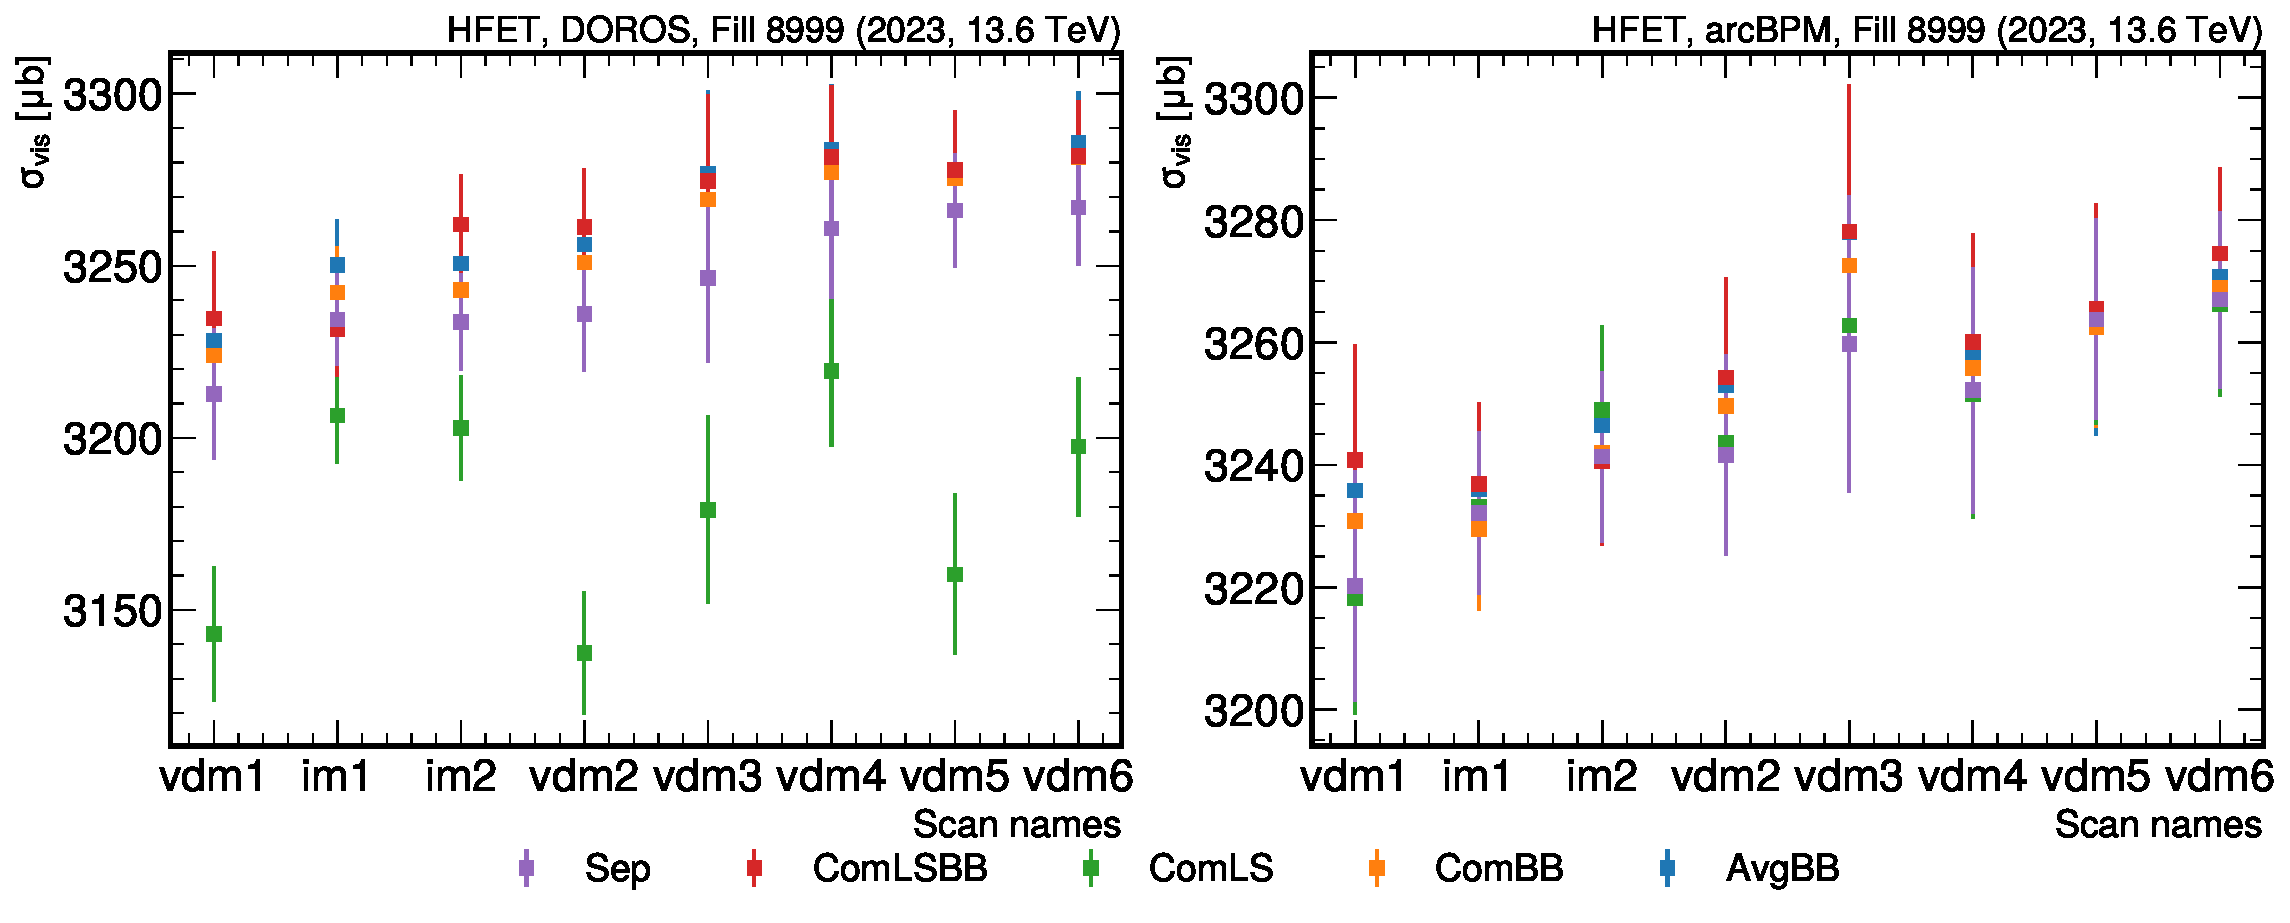
\includegraphics[width=0.8\paperwidth]{images/assets/rod_xsec_methods_results.pdf}}
	\caption[Comparison of residual orbit fit methods]{HFET visible cross section estimates for the vdM and im scan pairs after applying the orbit drift corrections. The central values are obtained by calculating the weighted average of the scan results. The scan to scan consistency is represented by the equivalent weighted standard deviation.}
	\label{fig:rod_xsec_methods_results}
\end{figure}

\begin{table}[!htb]
    \centering
    \caption{HFET visible cross-sections for the many residual fit methods for both arcBPM and DOROS systems.}
    \label{tb:hfet_rod_xsec}
    \begin{tabular}{lcc|cc}
        \hline
        \multirow{2}{*}{Method} & \multicolumn{2}{c|}{DOROS} & \multicolumn{2}{c}{arcBPM} \\
        \cline{2-5}
         & $\sigma_{\mathrm{vis}}$ [$\mu b$] & Uncertainty (\%) & $\sigma_{\mathrm{vis}}$ [$\mu b$] & Uncertainty (\%) \\
        \hline
        Sep     & 3243.48 & 0.53 & 3246.49 & 0.47 \\
        AvgBB   & 3262.38 & 0.56 & 3252.75 & 0.42 \\
        ComLS   & 3183.52 & 0.91 & 3247.55 & 0.46 \\
        ComBB   & 3255.48 & 0.58 & 3249.46 & 0.47 \\
        ComLSBB & 3260.45 & 0.59 & 3254.09 & 0.46 \\
        \hline
    \end{tabular}
\end{table}


The results obtained from the separately fit length scale parameters methods (Sep, AvgBB and ComBB) have not been considered since the length scale parameter as computed with the length scale calibration is constant throught the vdM program. The ComLSBB method with the measurements from the arcBPM system was chosen for its smaller scan-to-scan variation (0.46\%). This correction increased the visible cross-sections of all luminometers by 0.2\% with an associated uncertainty of 0.16\%, estimated from the standard deviation of results from all fits methods.

\subsection{XY factorization}

The assumption that the particle bunch distributions are factorizable in the tranverse plane has been kept throught all the previously mentioned corrections. Since this assumption is not guaranteed, the real visible cross-section differs from the one measured with \autoref{eq:calibration_from_fit_parameters} by what is referred to as the factorization bias. This bias is calculated by reconstructing the bunch overlap densities of the two beams during vdM fill, and comparing the results to the ones obtained from the one dimensional vdM scans.

Different methods are used for this purpose such as the beam-imaging method described in \cite{Klute_2017, knolle2019factorizationbiasvander, Knolle:442689}. For this analysis two other methods were used and their results were compared.

One of these methods is the 2D rate fit method, many times used in CMS \cite{CMS-PAS-LUM-18-002, CMS-PAS-LUM-22-001}. In this method, on-axis scans, like the already mentioned vdM and im scans, are combined with off-axis scans, such as diagonal and offset scans, that were performed close in time. In diagonal scans the scanning beam is moving in both the horizontal and vertical directions in a way that the scanning plane is at a 45º angle. Offset scans are like normal vdM scans with an additional separation in the non-scanning plane. These off-axis scans are illustrated in \autoref{fig:off_axis_scans}.

\begin{figure}[!htb]
	\centering
	\makebox[\textwidth]{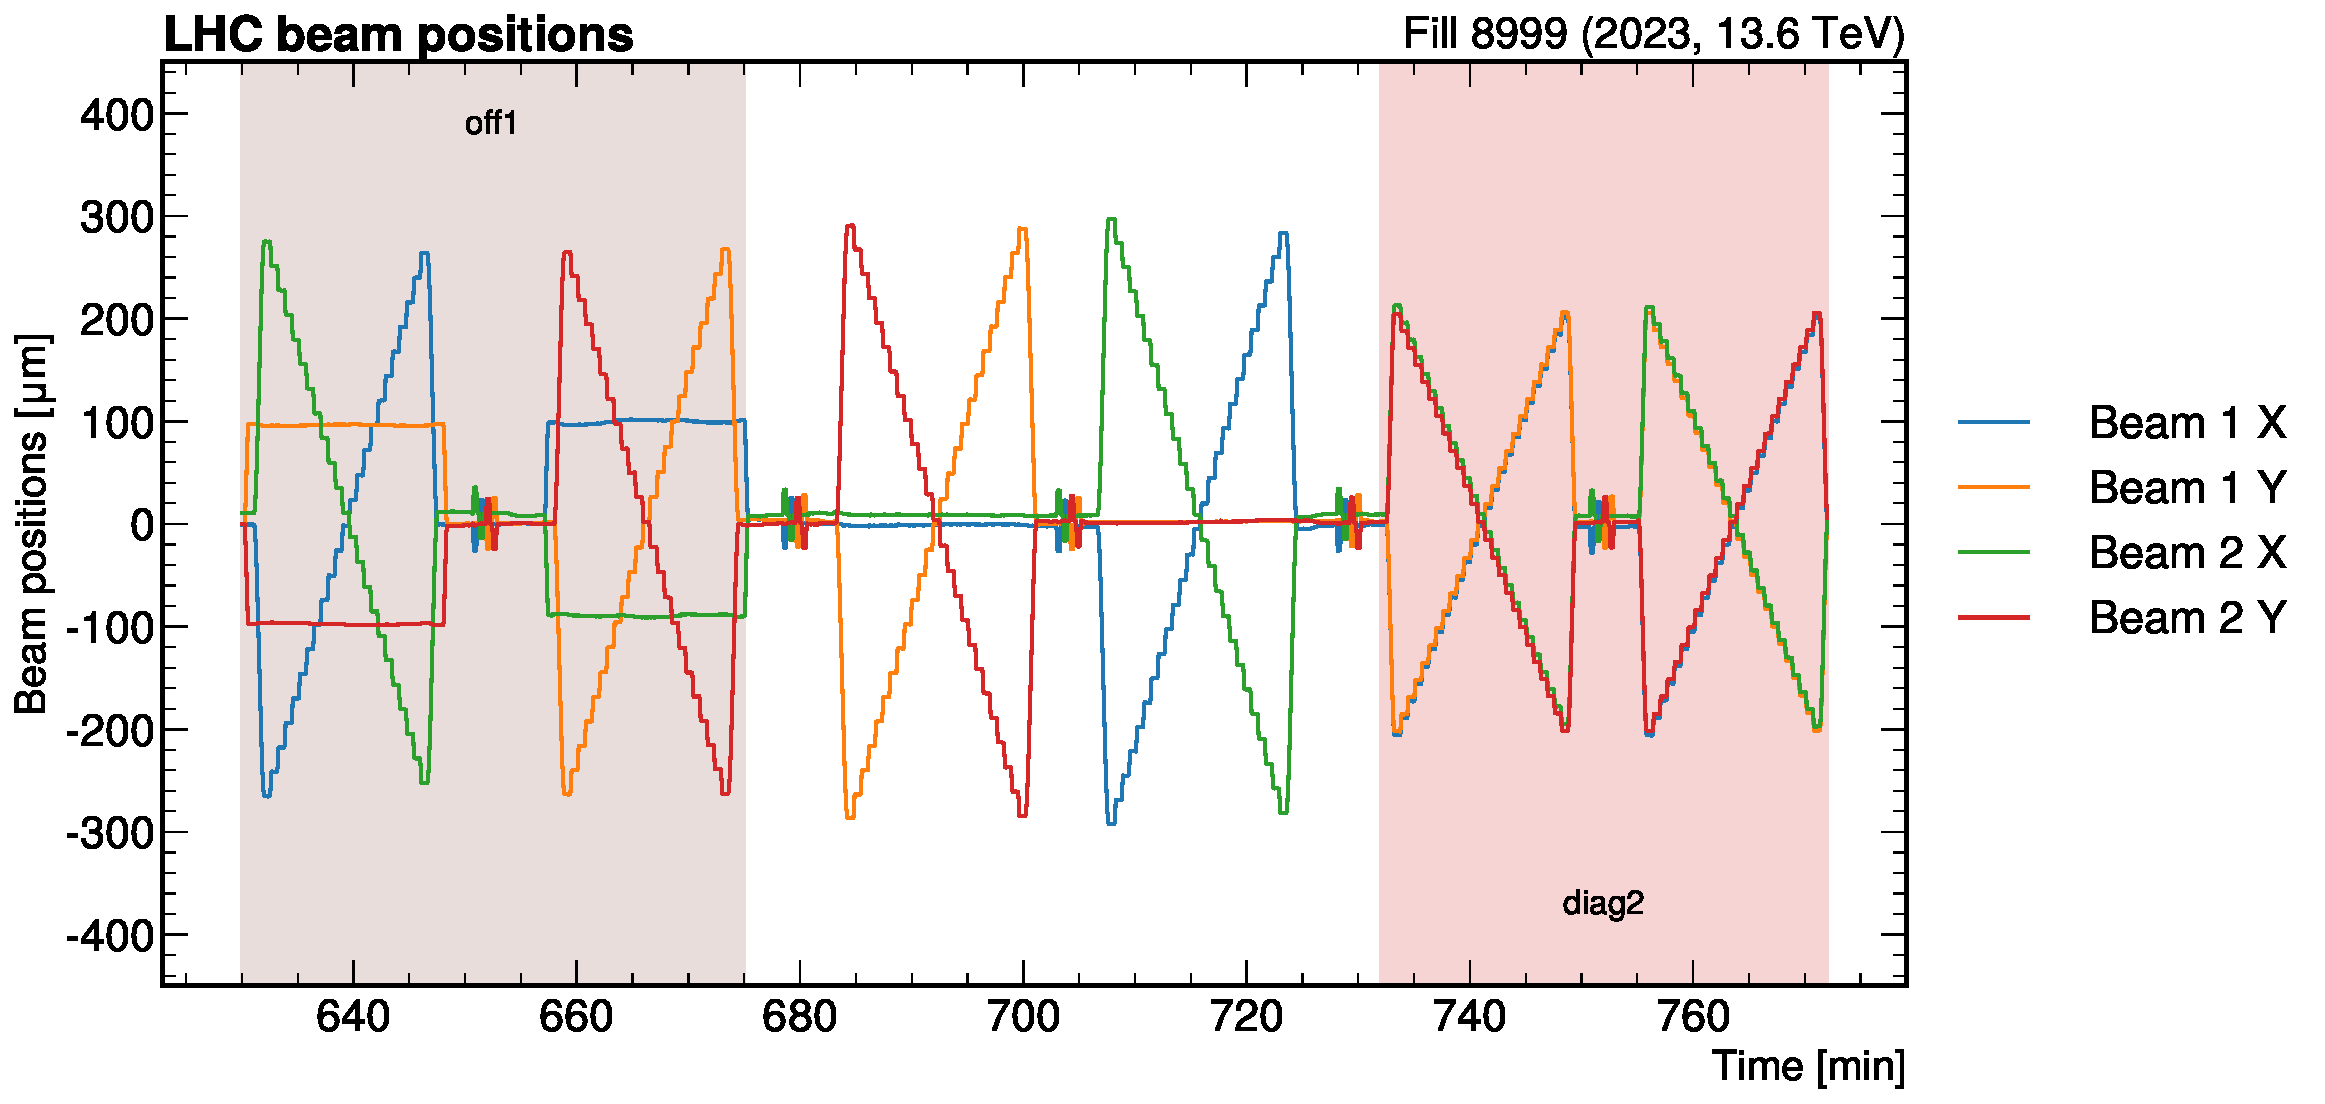
\includegraphics[width=0.8\paperwidth]{images/assets/off_axis_scans.pdf}}
	\caption{Beam positions during the first offset scan and the second diagonal scan of fill 8999.}
	\label{fig:off_axis_scans}
\end{figure}

The combination of on-axis with off-axis scans allows for the probing of the overlap bunch distribution along a different paths. This provides more information about the non-factorizable nature of this distribution. For the year of 2023 the scan combinations were vdM1+diag1, diag1+BI1, vdM3+off1, off1+vdM4, vdM4+diag2 and diag2+vdM5. The visible cross-section corrections for all these combinations are shown in \autoref{fig:2d_rate_fit_xsec_corrections}.

\begin{figure}[!htb]
	\centering
	\makebox[\textwidth]{\includegraphics[width=0.4\paperwidth]{images/assets/2d_rate_fit_xsec_corrections.png}}
	\caption[Factorization corrections on visible cross-section from 2D rate fit method]{Factorization corrections on the visible cross section from several on-axis scan - off-axis scan pairs as a function of time. The points from left to righ correspond to vdM1+diag1, diag1+BI1 combinations taken during the first part of the vdM program (in brown), and to vdM3+off, off+vdM4, vdM4+diag2, diag2+vdM5 combinations taken during the secon part of the vdM program (in purple). Over the nine hours of the data taking, the factorization correction changed from about 2.62\% to approximately 0.93\%, indicating a significant time dependence (from \textit{Ref.} \cite{CMS-DP-2024-068}).}
	\label{fig:2d_rate_fit_xsec_corrections}
\end{figure}

Lastly, in the luminous region a 3D fit is performed to luminometer rates using parameters of the 3D ellipsiod of the reconstructed beamspot and the bunch length data from the LHC LDM. One of the main advantages of this method in comparison to the 2D rate method is the ability to obtain cross section measurement for every vdM and im scan seperatly. For this reason, the corrections to the detectors calibration were derived from this method. A comparison to the 2D rate fit method is in \autoref{fig:luminous_region_vs_2d_rate_fit}, which shows the good agreement with both methods. The large time dependence in the correction values show the beam overlap shape changing throught the vdM fill.

\begin{figure}[!htb]
	\centering
	\makebox[\textwidth]{\includegraphics[width=0.5\paperwidth]{images/assets/luminous_region_vs_2d_rate_fit.png}}
	\caption[Factorization corrections on visible cross-section from luminous region method.]{Average correction for the visible cross section over nine BCIDs using five different models of the luminous region (LR) method. The scans are ordered in time. The averages include only BCIDs for which high-statistics zero bias samples are available, and the uncertainties indicate the RMS over these BCIDs. A small number of bad quality fits with anomalously large reduced $\chi^2$ > 5 values were discarded. Results for three models of the bunch proton density are shown: weighted sum of three (TG), four (QG) or five (PG) 3-dimensional Gaussians. The results – choosing the best and the second best (i.e. smallest) reduced $\chi^2$ fits from the nine tested models – are also given. On the right, the LR results are compared to the average corrections over 136 BCIDs using the 2D rate fit method (from \textit{Ref.} \cite{CMS-DP-2024-068}).}
	\label{fig:luminous_region_vs_2d_rate_fit}
\end{figure}

The XY-factorization bias was the main responsible for reducing the scan-to-scan variation seen in \autoref{fig:no_Corr_xsec_results_HFET} and \autoref{fig:no_Corr_xsec_results_HFET}. The total uncertainty for this correction is 0.67\. This was estimated from the uncertainty associated with model and BCID dependence, maximum discrepancy with 2D rate fit method among other sources \cite{CMS-PAS-LUM-22-001}.

\subsection{Calibration results}

The visible cross-section results were determined by performing a weighted average on the calibrations measured in the eight analyzed scans, incorporating all prior corrections. \autoref{tab:xsec_summary} provides a summary of the results for all independently calibrated luminometers, along with their associated uncertainties. The associated $\sigma_{\mathrm{vis}}$ evolution plots are in \autoref{fig:all_Corr_xsec_results_HFET} for the HFET detector and in \autoref{fig:all_Corr_luminometer_xsec} and \autoref{fig:cross_section_results_pcc} for the remaining luminometers.

\begin{table}[!htb]
	\caption[Summary of visible cross-sections results]{Summary of the measured visible cross sections. The results have been computed through a average weighted on the error of each scan and are accompanied by their standard error on the mean. The bunch-to-bunch uncertainty range across all scans is shown in the "Bunches RMS" column. The "Scans RMS" depicts the overall scan-to-scan variation. }
	
	\label{tab:xsec_summary}
	\centering
	\begin{tabular}{lcccc}
		\hline
		Luminometer & Measured $\sigma_\mathrm{vis}$ & SEM  & Bunches RMS & Scans RMS \\
		\hline
		BCM1F & 136.36 $\mu b$ & 0.17 $\mu b$ & 0.58-1.03 $\mu b$ (0.43-0.76\%) & 0.41 $\mu b$ (0.30\%) \\
		BCM1FUTCA & 127.55 $\mu b$ & 0.15 $\mu b$ & 0.61-1.09 $\mu b$ (0.48-0.85\%) & 0.40 $\mu b$ (0.31\%) \\
		HFET & 3294.69 $\mu b$ & 3.86 $\mu b$ & 12.82-21.78 $\mu b$ (0.39-0.66\%) & 9.28 $\mu b$ (0.28\%) \\
		HFOC & 946.05 $\mu b$ & 1.12 $\mu b$ & 2.49-5.92 $\mu b$ (0.26-0.63\%) & 2.63 $\mu b$ (0.28\%) \\
		PLT & 301.39 $\mu b$ & 0.37 $\mu b$ & 1.52-2.38 $\mu b$ (0.50-0.79\%) & 0.90 $\mu b$ (0.30\%) \\
		PCC & 1305.23 $mb$ & 1.21 $mb$ & 3.31-8.85 $mb$ (0.25-0.68\%) & 3.27 $mb$ (0.25\%) \\
		\hline
	\end{tabular}
\end{table}

\begin{figure}[!htb]
	\centering
	\makebox[\textwidth]{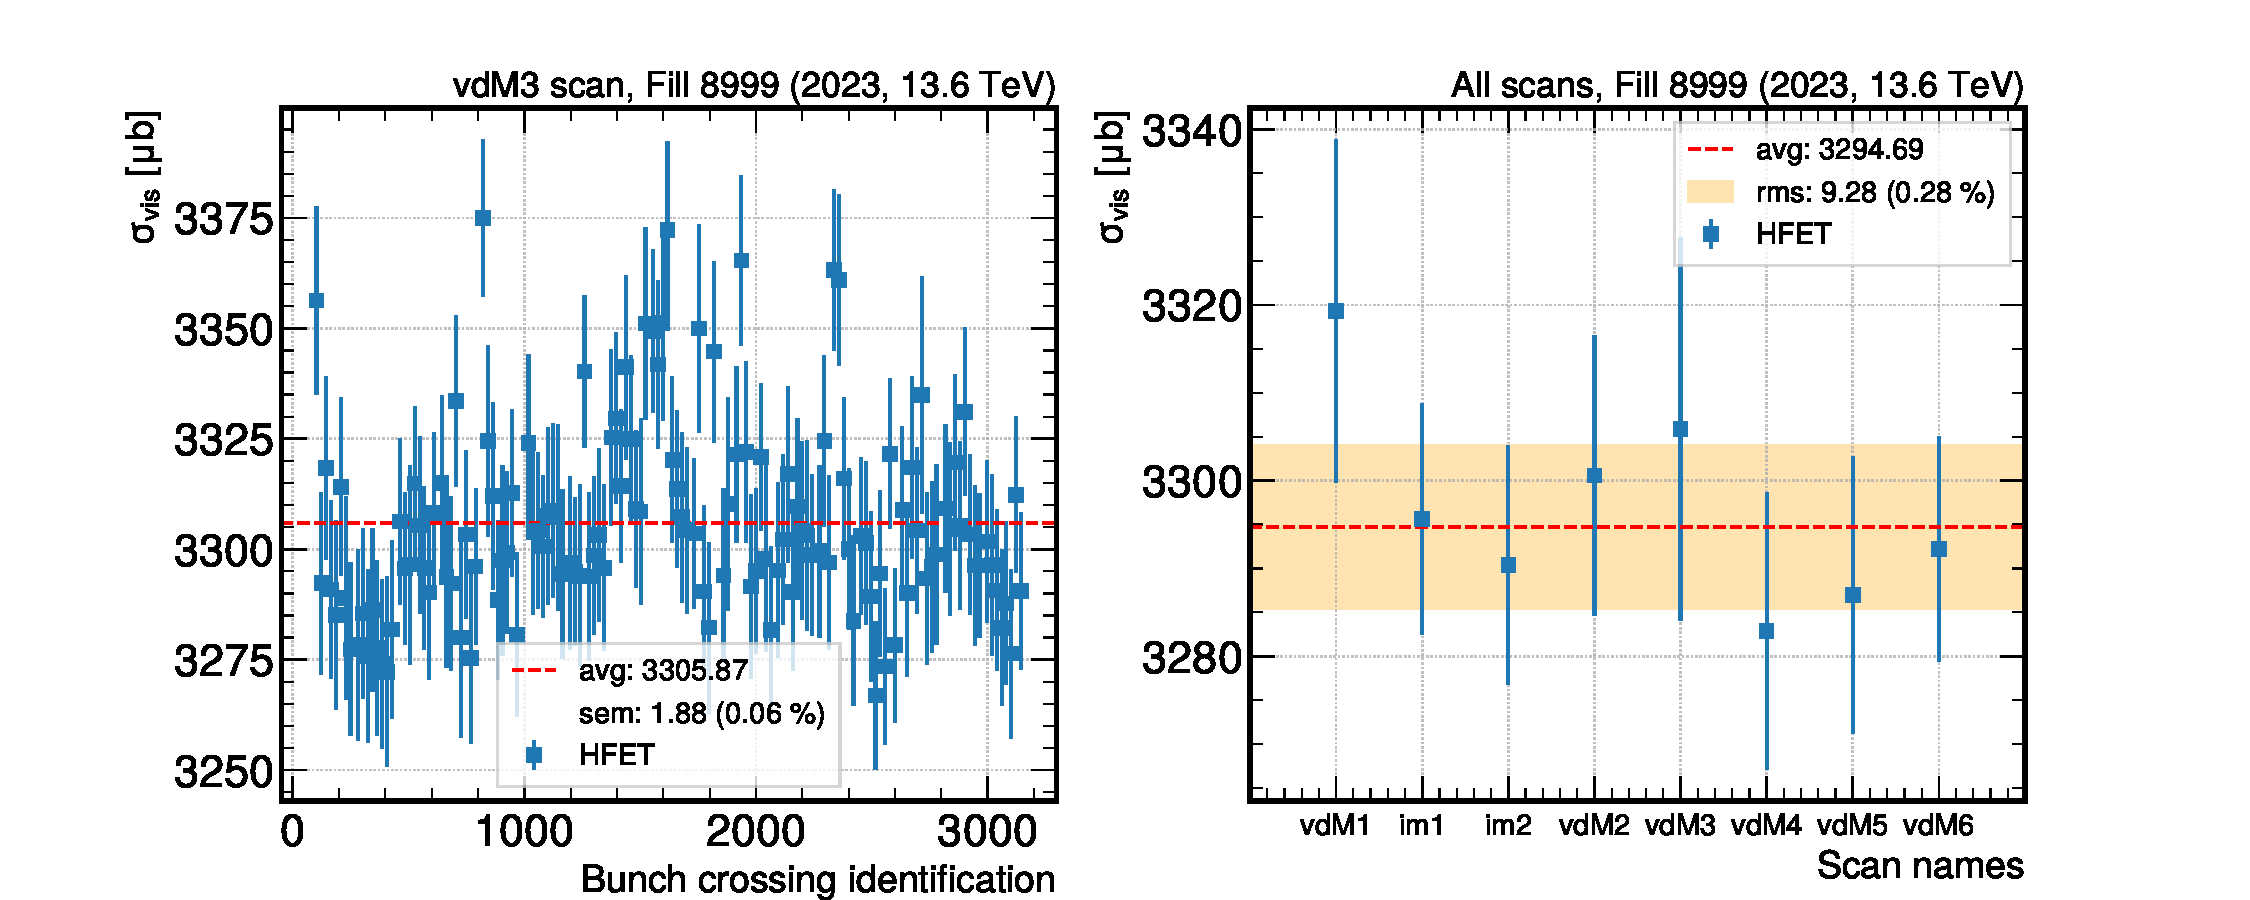
\includegraphics[width=0.9\paperwidth]{images/assets/all_Corr_xsec_results_HFET.pdf}}
	\caption[Final HFET cross-section results]{Final cross-section results obtained after all data corrections for the HFET luminometer as an example. On the left, the measured per-bunch visible cross-sections with his associated fit uncertainty are shown. The right image shows the measured visible cross-section taking the average over all 136 BCIDs for each vdM and im scan pairs. All statistics are determined as in \autoref{fig:no_Corr_xsec_results_HFET}.}
	\label{fig:all_Corr_xsec_results_HFET}
\end{figure}

\begin{figure}[!htb]
	\centering
	\makebox[\textwidth]{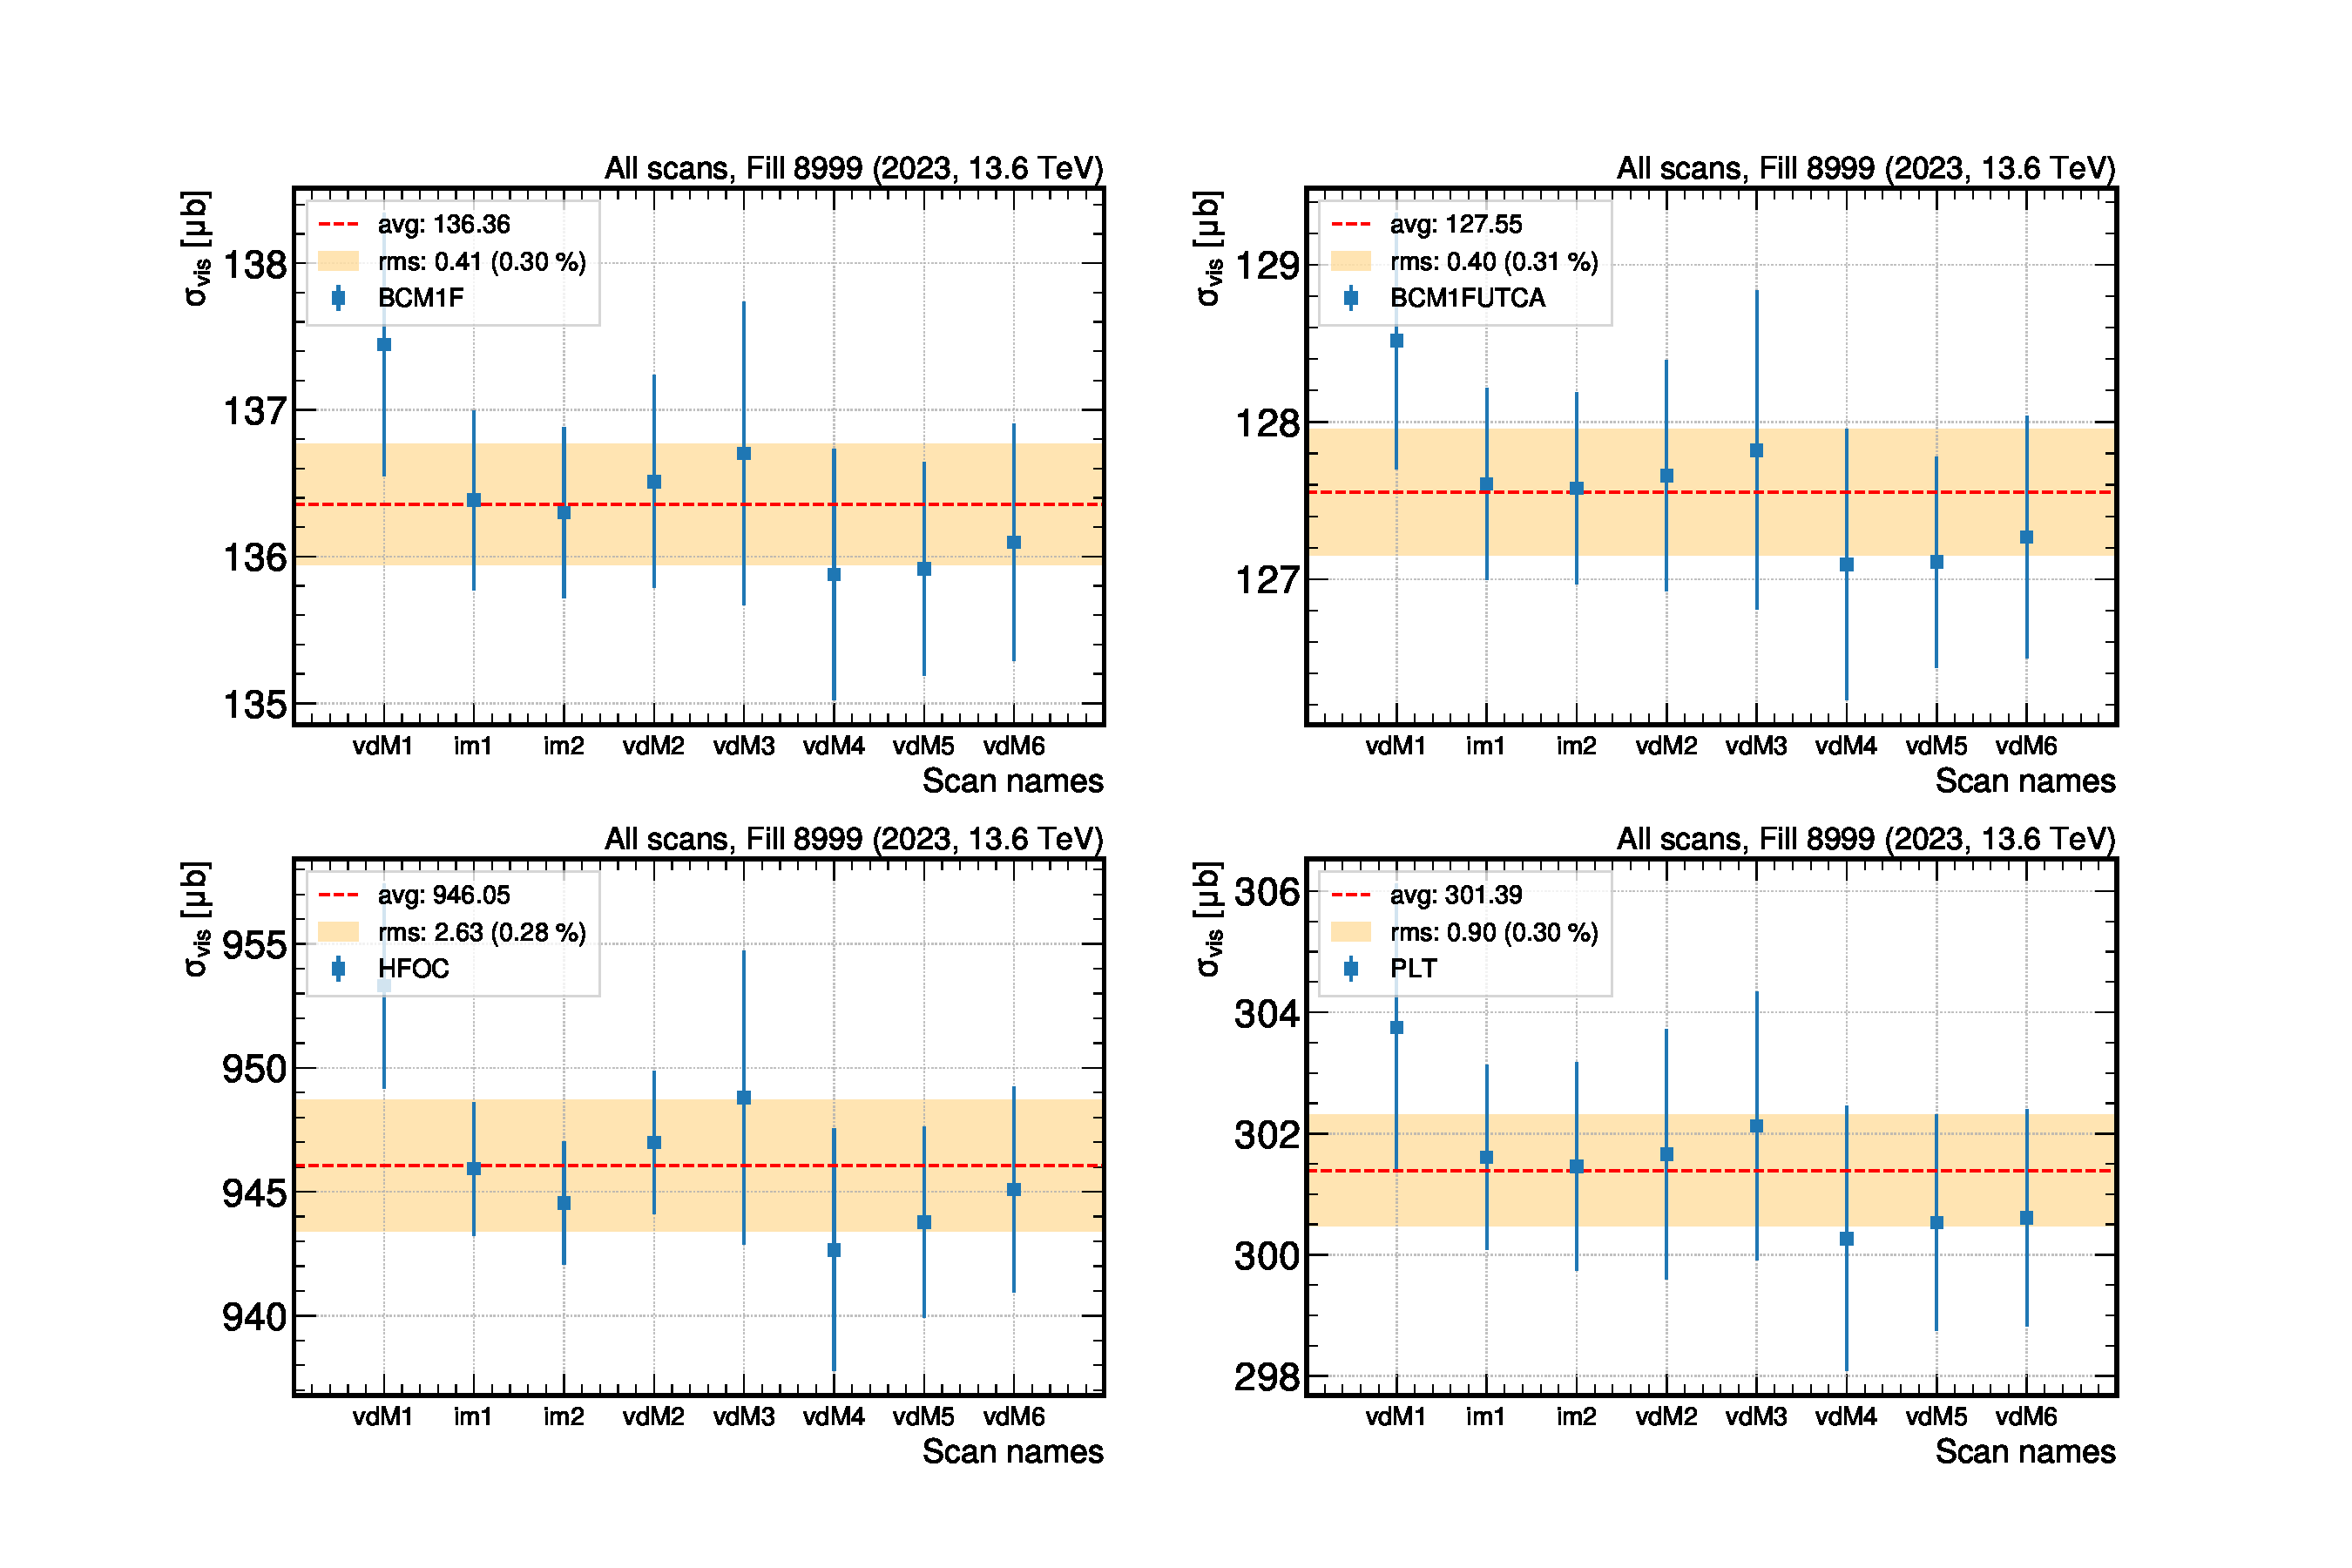
\includegraphics[width=0.7\paperwidth]{images/assets/all_Corr_luminometer_xsec.pdf}}
	\caption[Final cross-section results for other online luminometers]{Final cross-section results obtained after data corrections for BCM1F, BCM1FUTCA, HFOC and PLT luminometers.}
	\label{fig:all_Corr_luminometer_xsec}
\end{figure}

\begin{figure}[!htb]
	\centering
	\makebox[\textwidth]{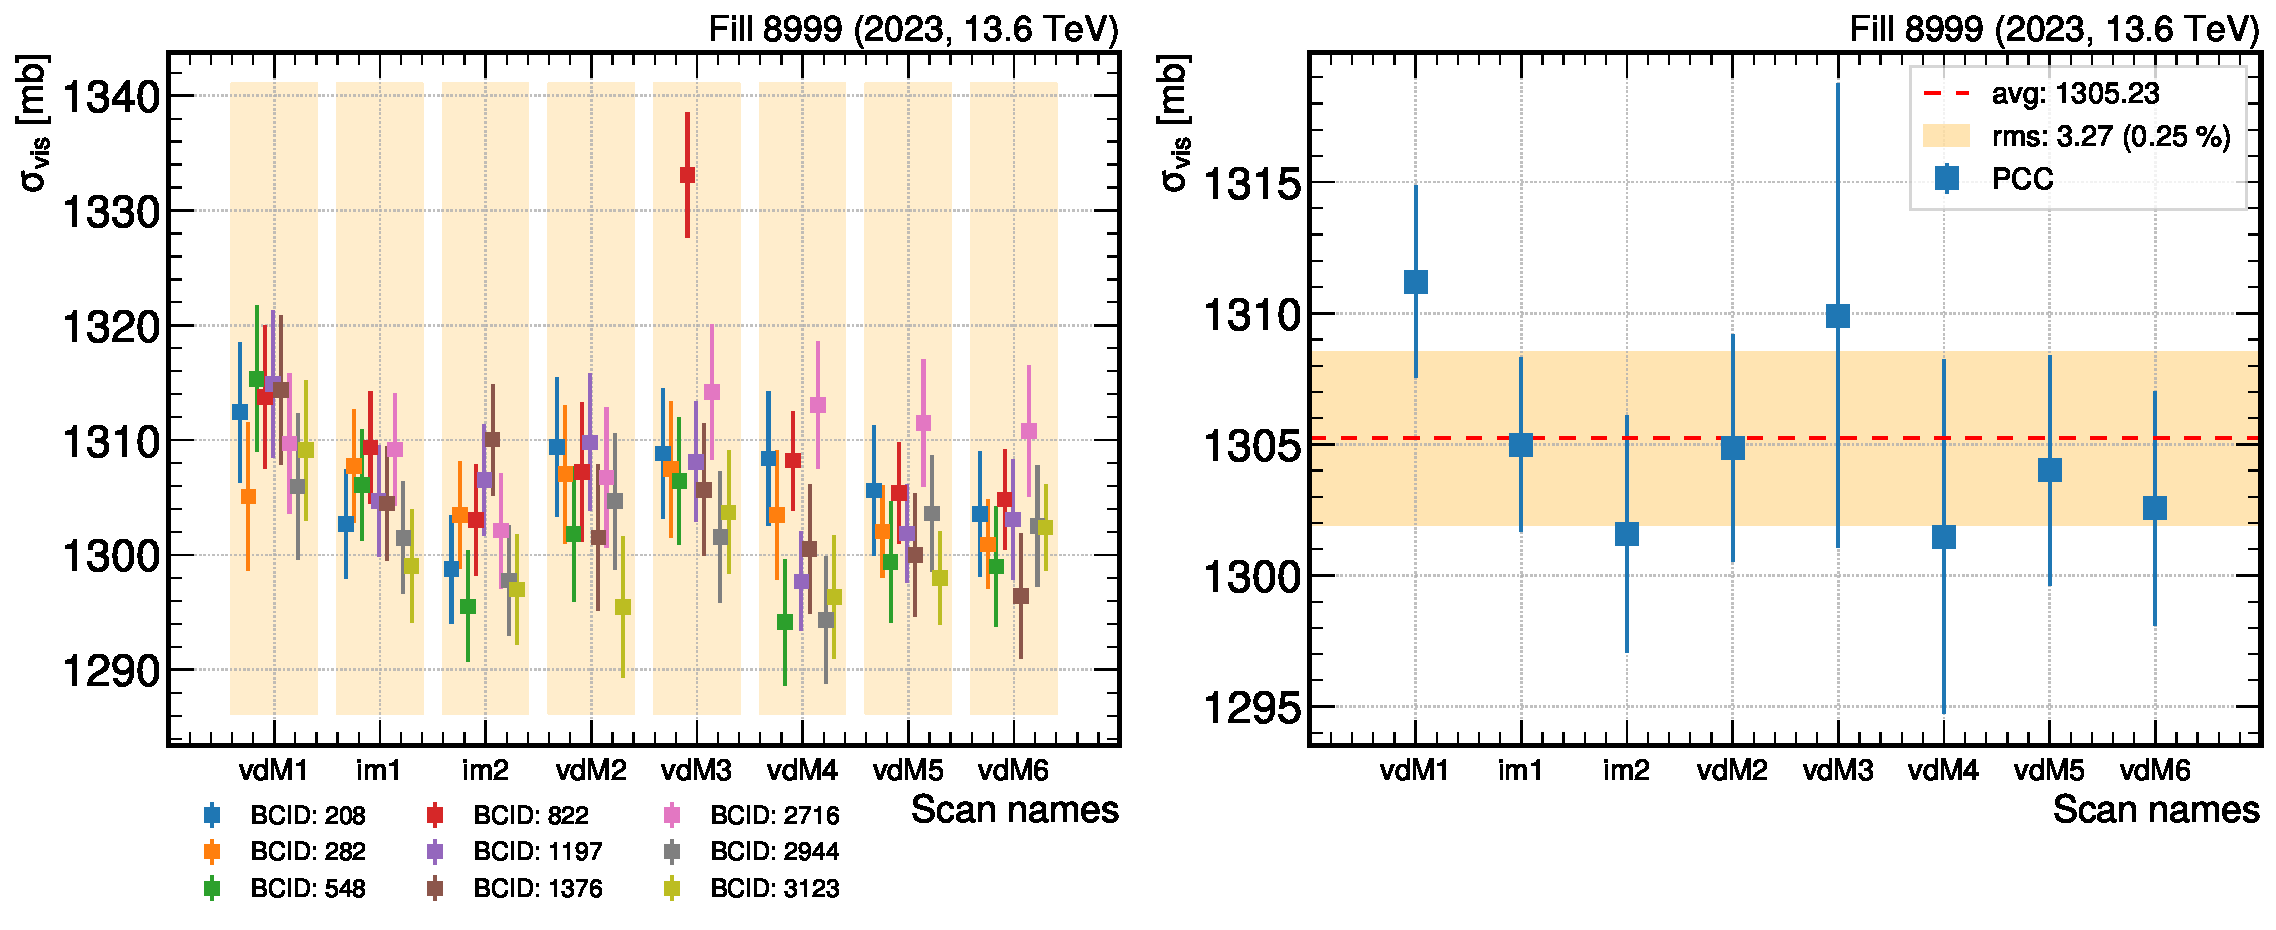
\includegraphics[width=0.6\paperwidth]{images/assets/cross_section_results_pcc.pdf}}
	\caption[PCC calibration results]{The left plot shows the PCC calibration results for all the vdM fill scans and recorded BCIDs, which are 208, 282, 548, 822, 1197, 1376, 2716, 2944, and 3123. The right displays the PCC scan-to-scan variation across all vdM and im scans.
	}
	\label{fig:cross_section_results_pcc}
\end{figure}

The bunch-to-bunch variation in the cross-section measurements is attributed as a source of uncertainty and has a magnitude of 0.6\%, the standard deviation of the mean of HFET. Similarly, the calibration variation across scans as also used as another degree of uncertainty. HFET's weighted RMS across all scans, 0.28\%, was the attributed uncertainty.

The fit results were compared among the different luminometers and their individual reduced $\chi^2$ per scanning plane were plotted for all vdM scans. Overall, the results report good fit quality for both axis, with fits performed on HFOC reporting to have slightly higher reduced $\chi^2$ in the vertical plane. An example of the fits for the BCM1FUTCA detector is shown in \autoref{fig:fit_BCM1FUTCA_103} and the distributions for all online luminometers can be seen in \autoref{fig:chi2_distributions}.

\begin{figure}[!htb]
	\centering
	\makebox[\textwidth]{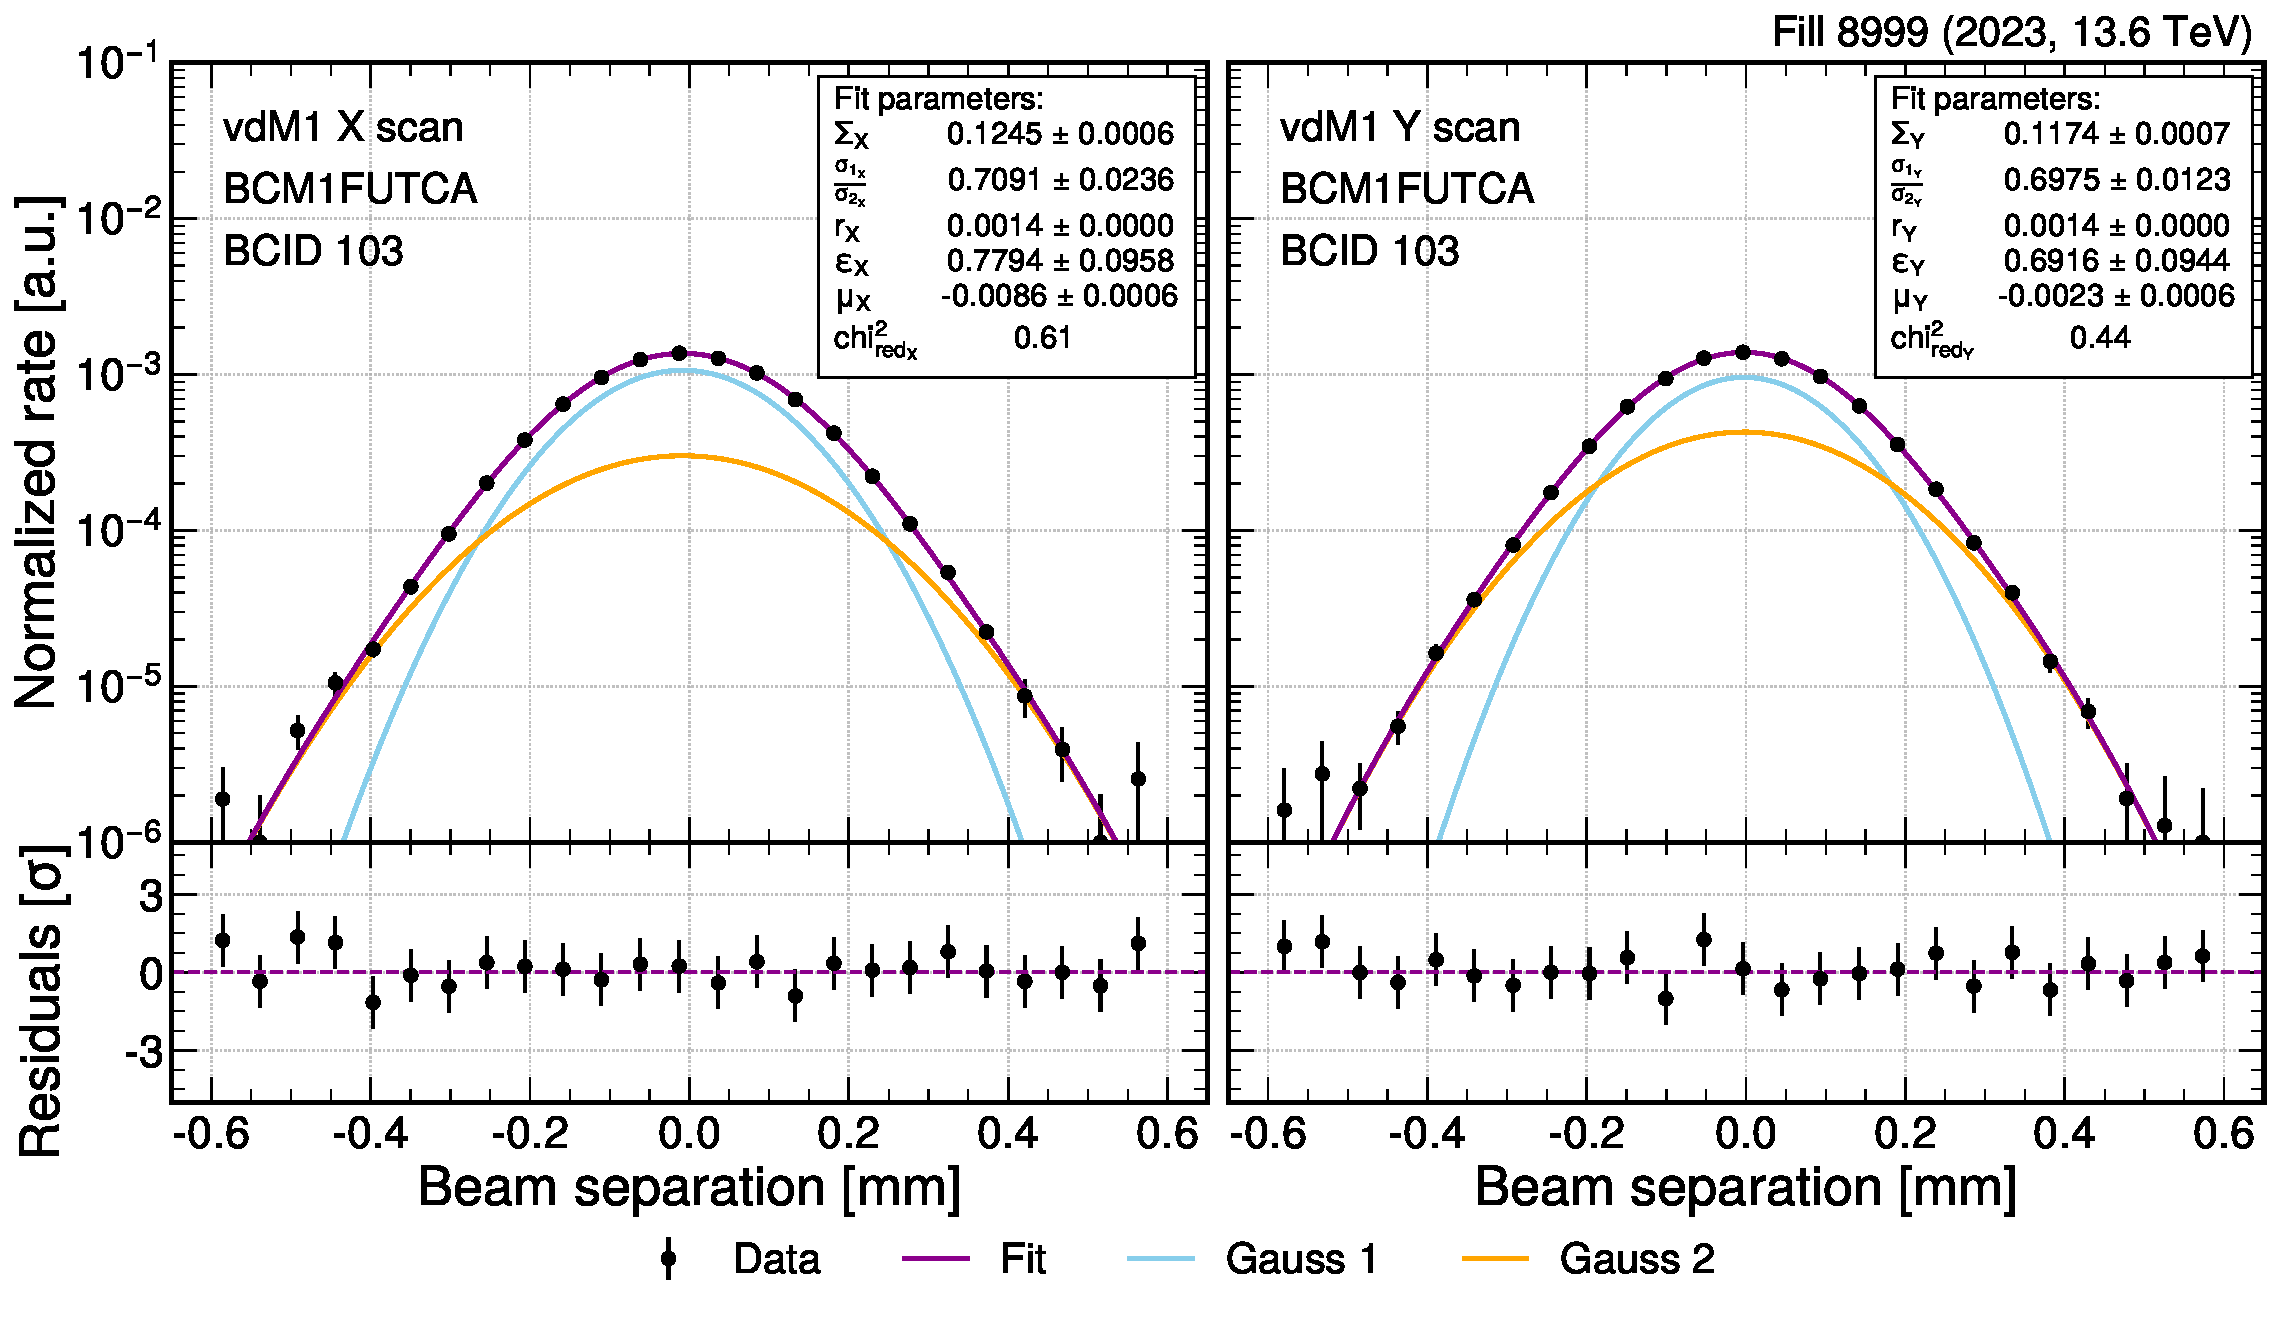
\includegraphics[width=0.7\paperwidth]{images/assets/fit_BCM1FUTCA_103.pdf}}
	\caption[Double Gaussian fits for BCM1FUTCA]{Double Gaussian fits to the BCM1FUTCA data recorded during the first vdM scanpair (vdM1), shown for the x (left) and y (right) scan. In the bottom panels, the statistical pull for each datapoint is shown. The boxes indicate the fit parameters for the fit in question. From top to bottom these contain the bunch overlap width, the ratio between both gaussians, the rate at the peak, the weight factor for the first gaussian curve, the mean of the overall distribution and the reduced $\chi^2$.}
	\label{fig:fit_BCM1FUTCA_103}
\end{figure}

\begin{figure}[!htb]
	\centering
	\makebox[\textwidth]{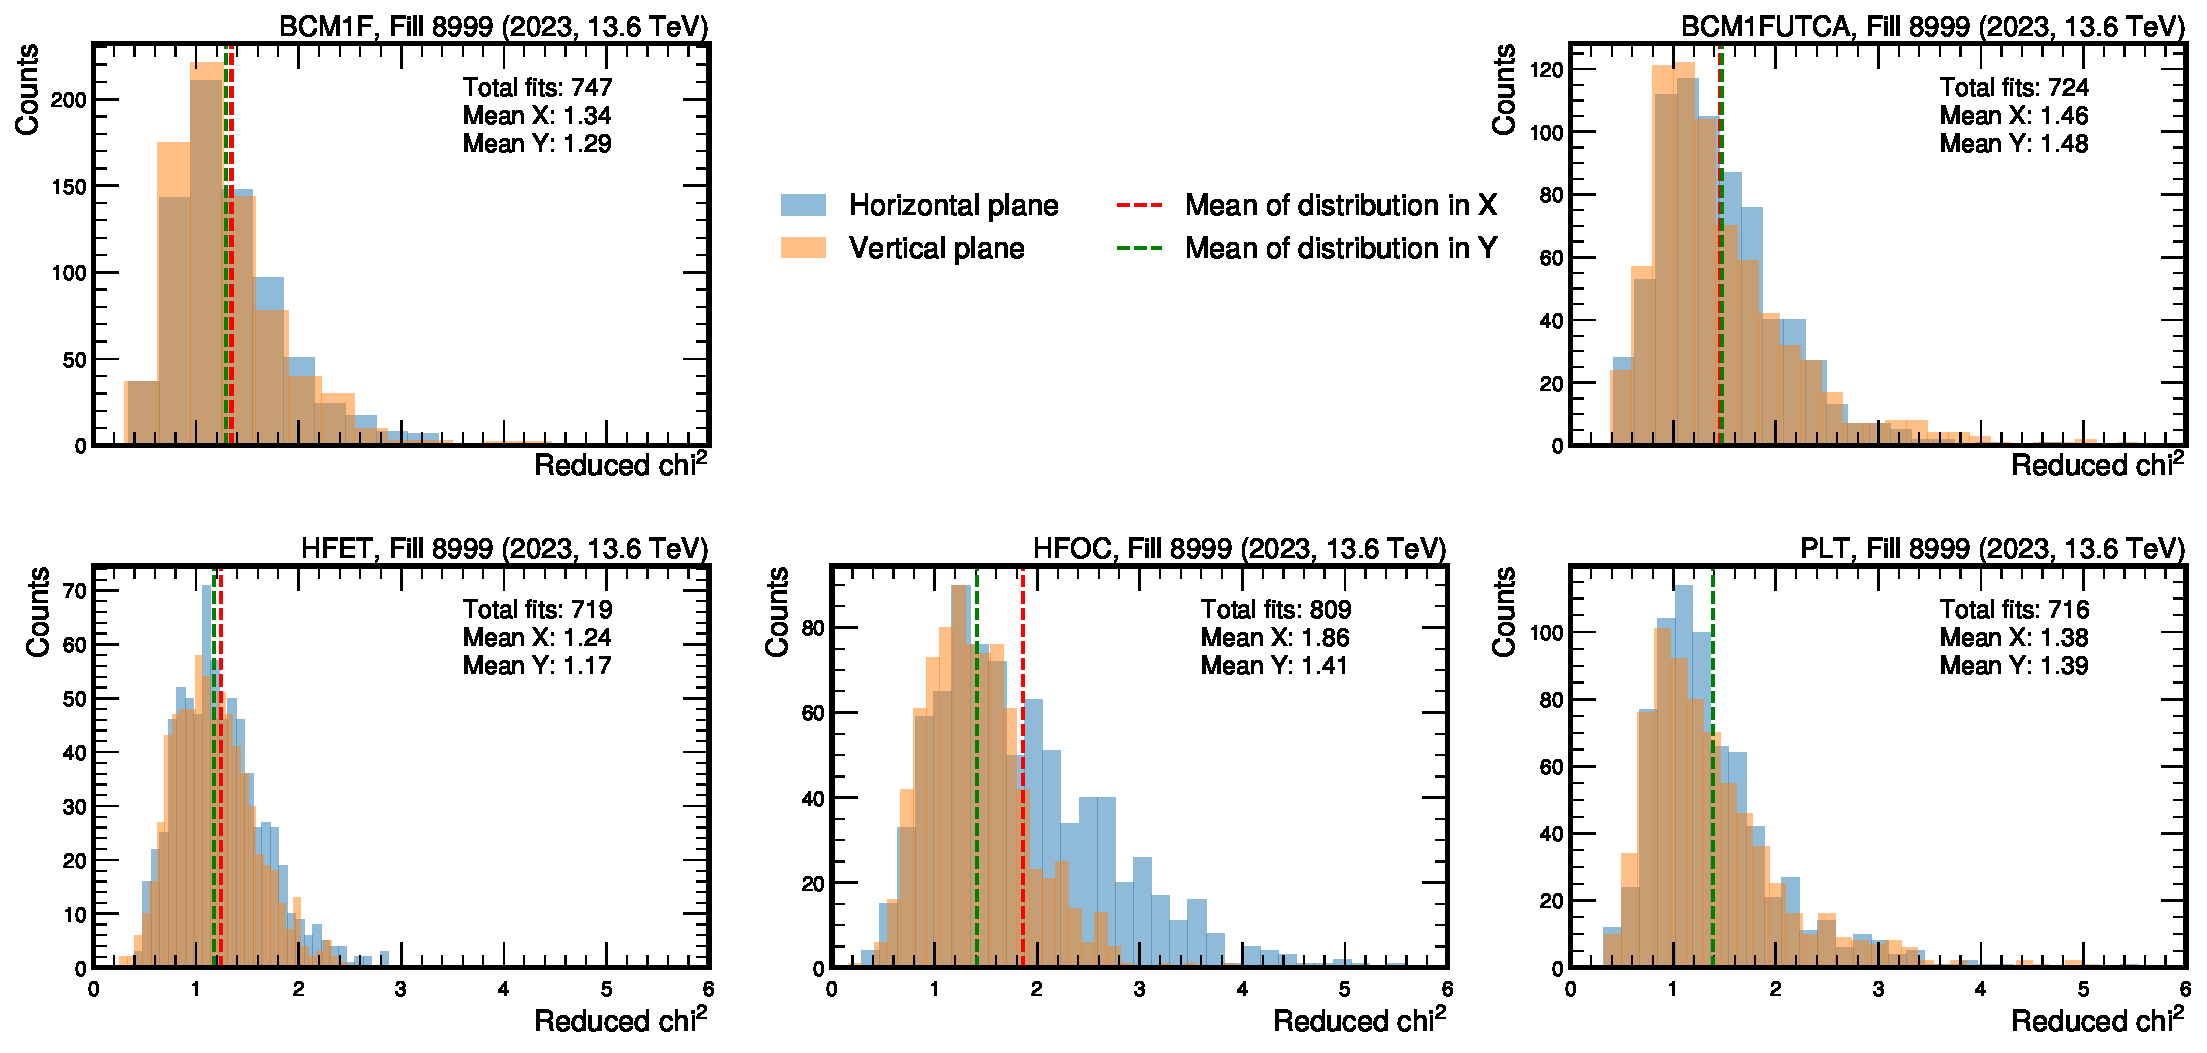
\includegraphics[width=0.7\paperwidth]{images/assets/chi2_distributions.pdf}}
	\caption[Scan fits reduced $\chi^2$ distribution]{Overview of the reduced $\chi^2$ distributions for all online luminometers for both scanning planes and all vdM scans. Only converged fits are considered which leads to a slightly different total number of fits per detector.}
	\label{fig:chi2_distributions}
\end{figure}

It's with these fits that we extract the measured the effective width and height of the luminous area, $\Sigma_X$ and $\Sigma_Y$, for all of the luminometers. Has it is a property of each bunch-pair, defined by their emittances and the constant $\beta^{*}$ at CMS, it should be consistent for all luminometers. The comparison is shown in \autoref{fig:capsigma_vdm1} and \autoref{fig:capsigma_evol}, and good agreement is observed. In the latter figure, the time-evolution of beam emittances can be observed.

\begin{figure}[!htb]
	\centering
	\makebox[\textwidth]{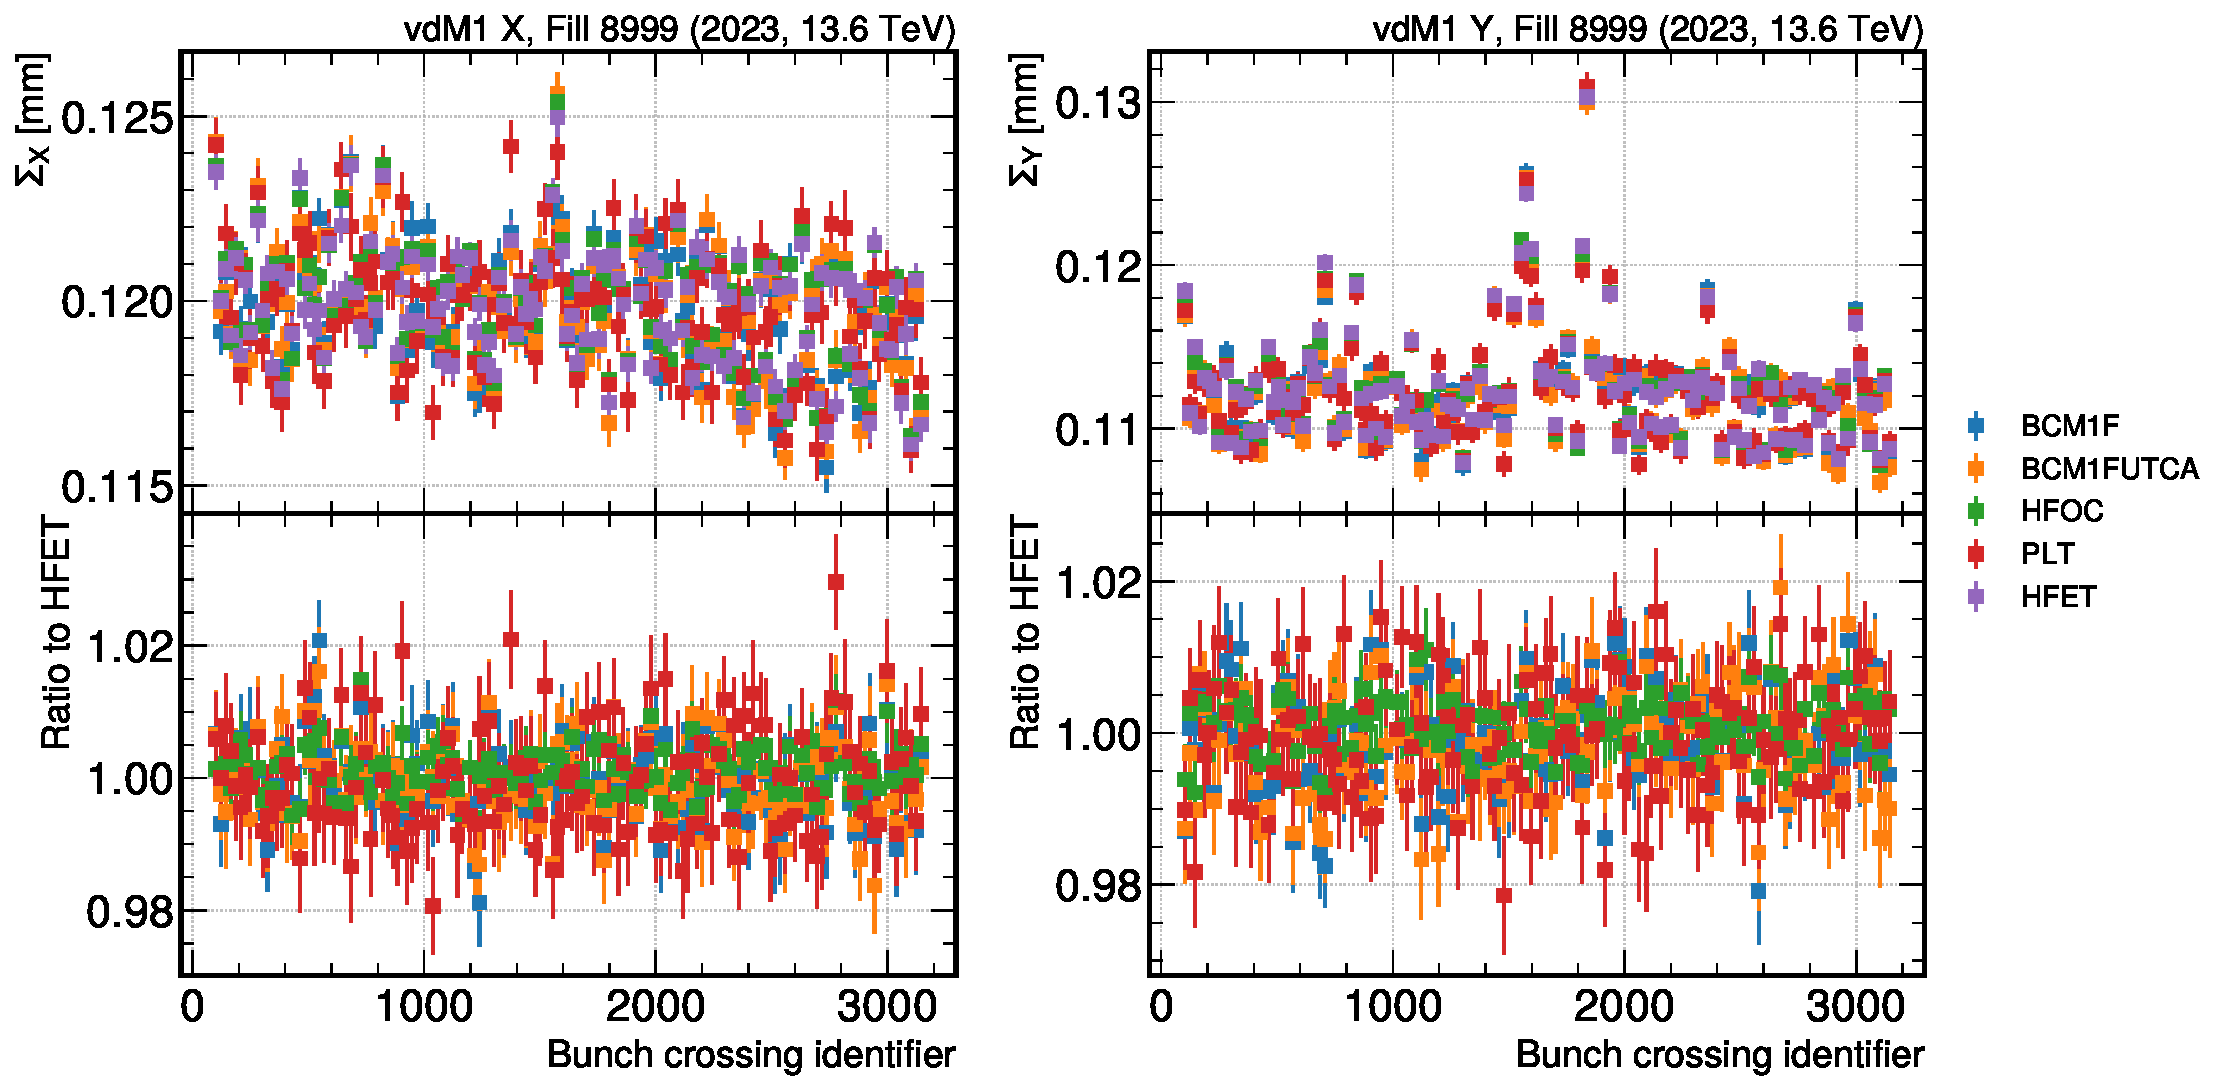
\includegraphics[width=0.6\paperwidth]{images/assets/capsigma_vdm1.pdf}}
	\caption[Overview of the measured effective beam overlap widths]{Overview of the $\Sigma$ results measured during the vdM1 scan pair, by all the online luminometers (upper row). Ratios of the measured values by different systems with respect to HFET are also shown (bottom row).}
	\label{fig:capsigma_vdm1}
\end{figure}

\begin{figure}[!htb]
	\centering
	\makebox[\textwidth]{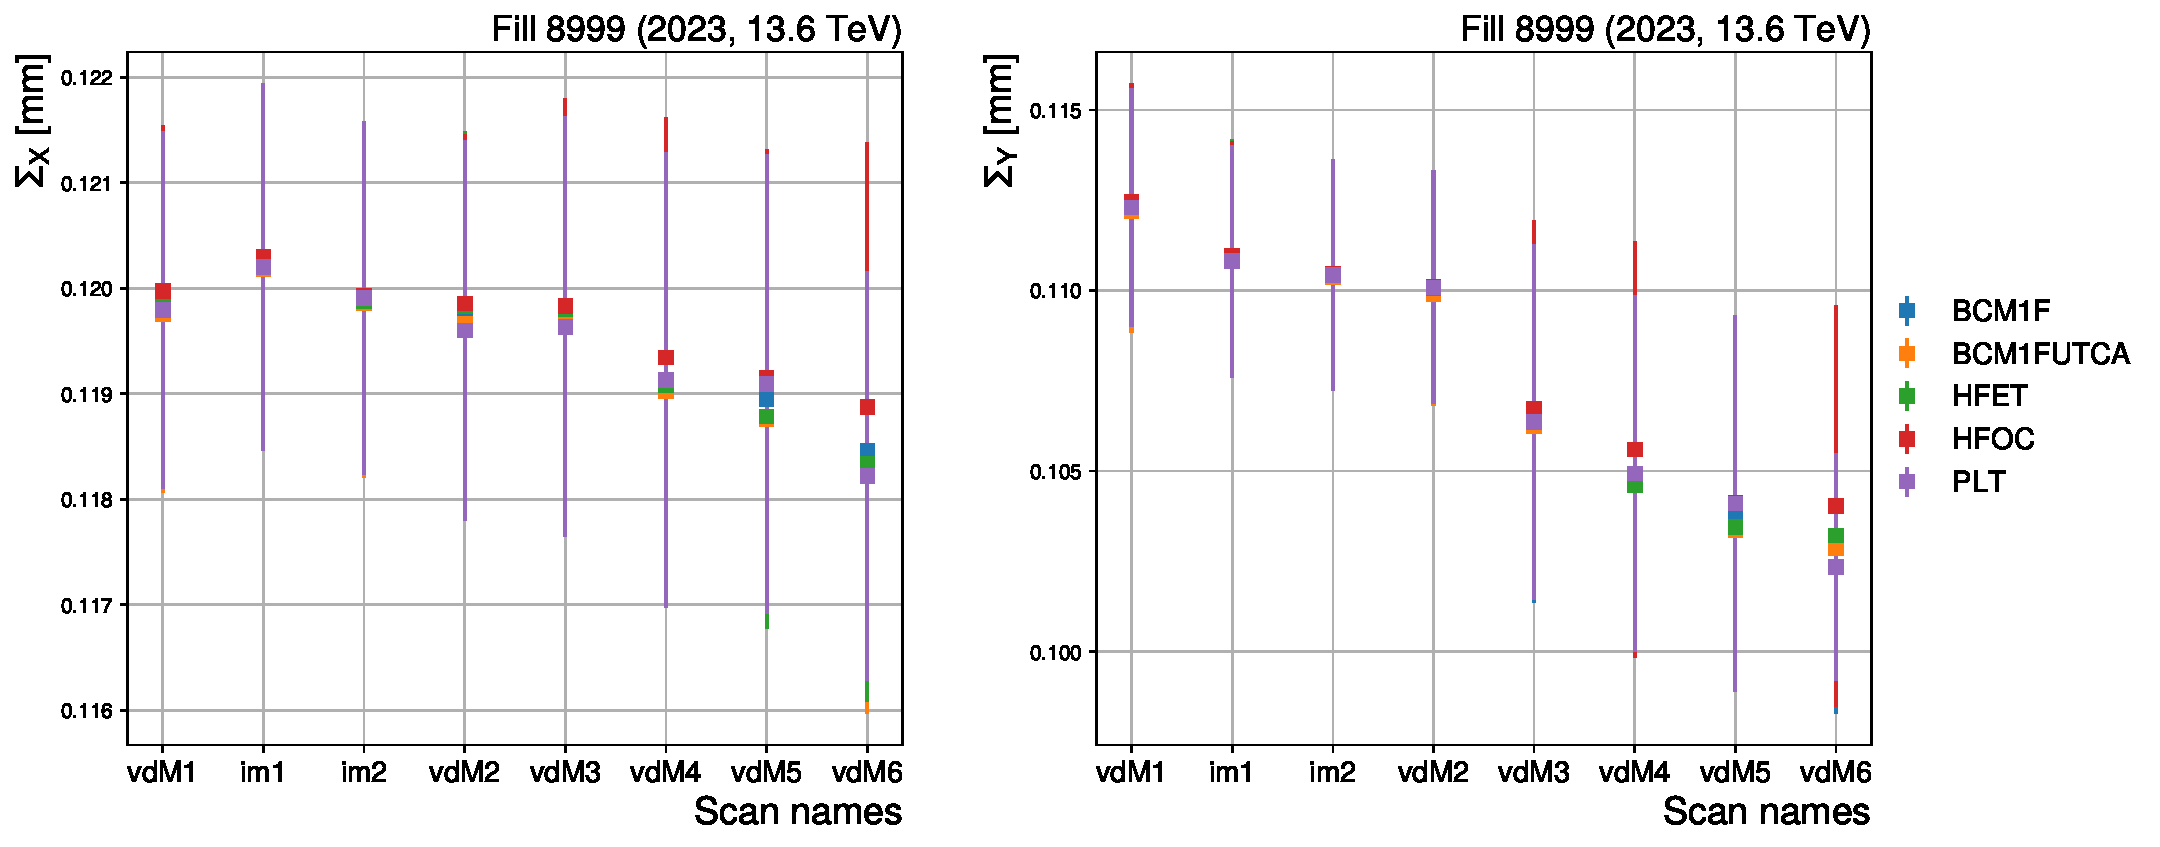
\includegraphics[width=0.6\paperwidth]{images/assets/capsigma_evol.pdf}}
	\caption{Overview of the average $\Sigma$ values in both transverse plans measured during all vdM and im scans, by all the online luminometers.}
	\label{fig:capsigma_evol}
\end{figure}

\newpage

\section{Integration}

In the previous section, the process by which the detector calibration factors were obtained was discussed. In this section, I will evaluate the performance of these calibrations in maximizing luminosity agreement between luminometers during the vdM fill and, more importantly, under physics conditions. A discussion on the year-long detector consistency will be presented, along with details on the specific stability corrections applied to the BCM1F. Additionally, the issue of detector non-linearity will be addressed, focusing on the PLT corrections. Finally, this section will present the final integrated luminosity for 2023, along with the associated relative uncertainty.

\newpage

\subsection{vdM Consistency}
\label{subsec:vdm_consistency}

Using the calibration values shown in \autoref{tab:xsec_summary}, the measured luminosity of each independently calibrated detector can be compared to visualize the detector agreement under vdM conditions. \autoref{fig:vdm_instantaneous_lumi_vs_time} shows the instantaneous luminosity throughout the entire vdM program.

\begin{figure}[!htb]
	\centering
	\makebox[\textwidth]{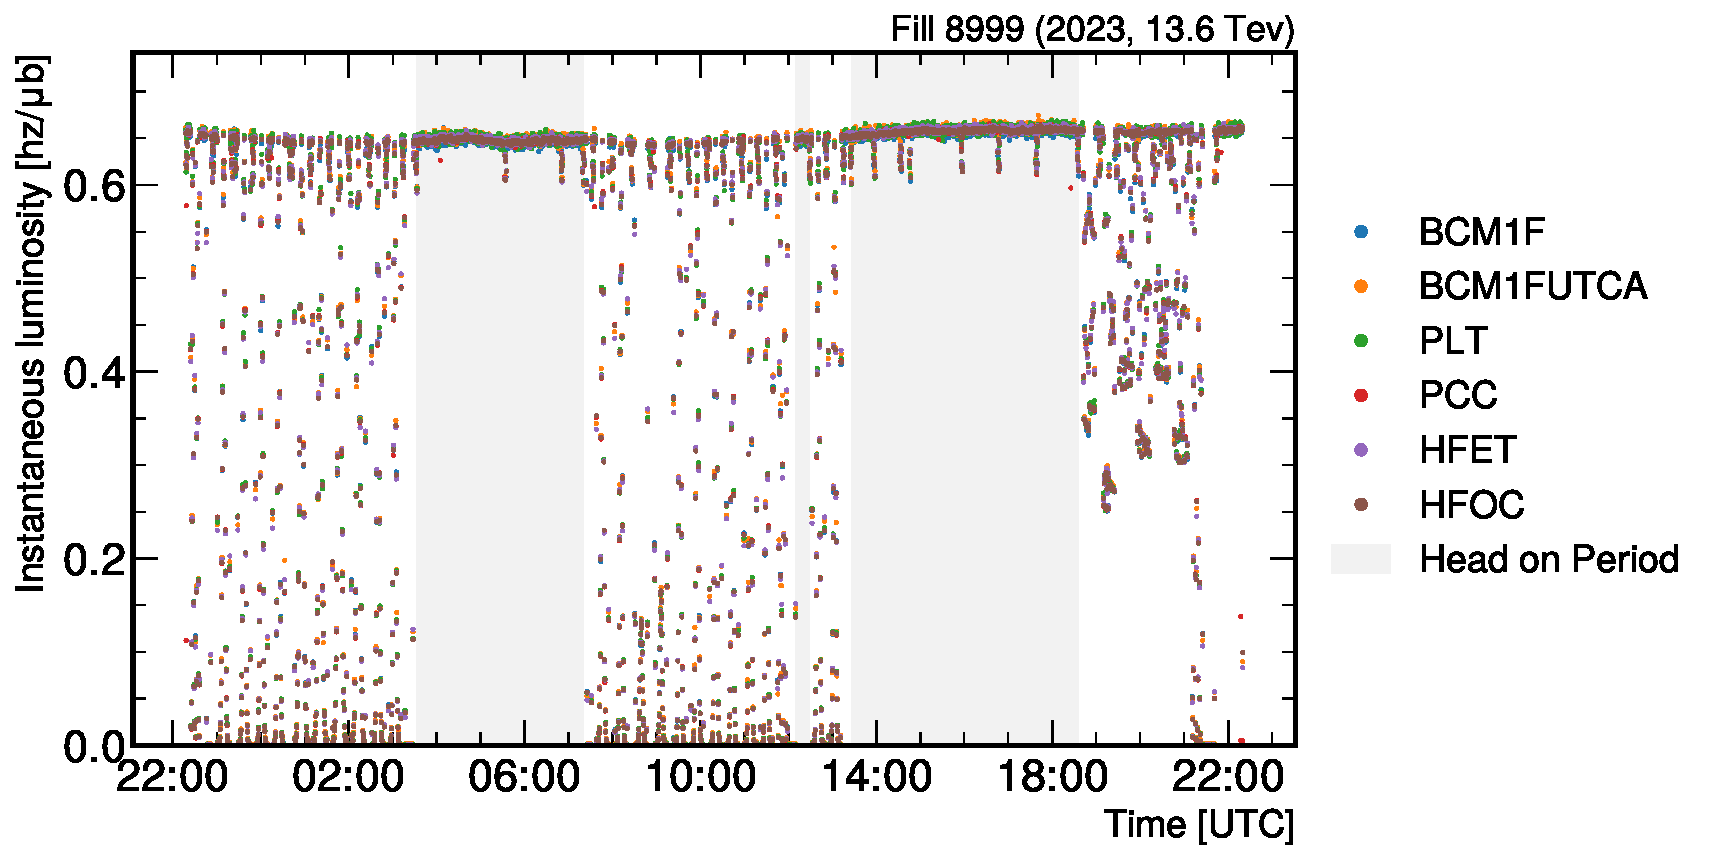
\includegraphics[width=0.6\paperwidth]{images/assets/vdm_instantaneous_lumi_vs_time.pdf}}
	\caption[Instantaneous luminosity during vdM]{Measured instantaneous luminosity as a function of time during the vdM program. All independently calibrated luminometers are present and show good agreement, especially during the head-on periods marked by the light grey areas.}
	\label{fig:vdm_instantaneous_lumi_vs_time}
\end{figure}

The luminometers show very good agreement with each other. The cross-detector consistency during the vdM fill was evaluated from the head-on ratios of all the luminometers with respect to the overall average. \autoref{fig:vdm_head_on_lumi_vs_time_and_ratio} shows the agreement of the luminometers during these periods in the vdM fill. The overall spread of the detectors was taken as the standard deviation of the means, with a magnitude of 0.16\% (see \autoref{fig:vdm_ratio_histograms}).

\begin{figure}[!htb]
	\centering
	\makebox[\textwidth]{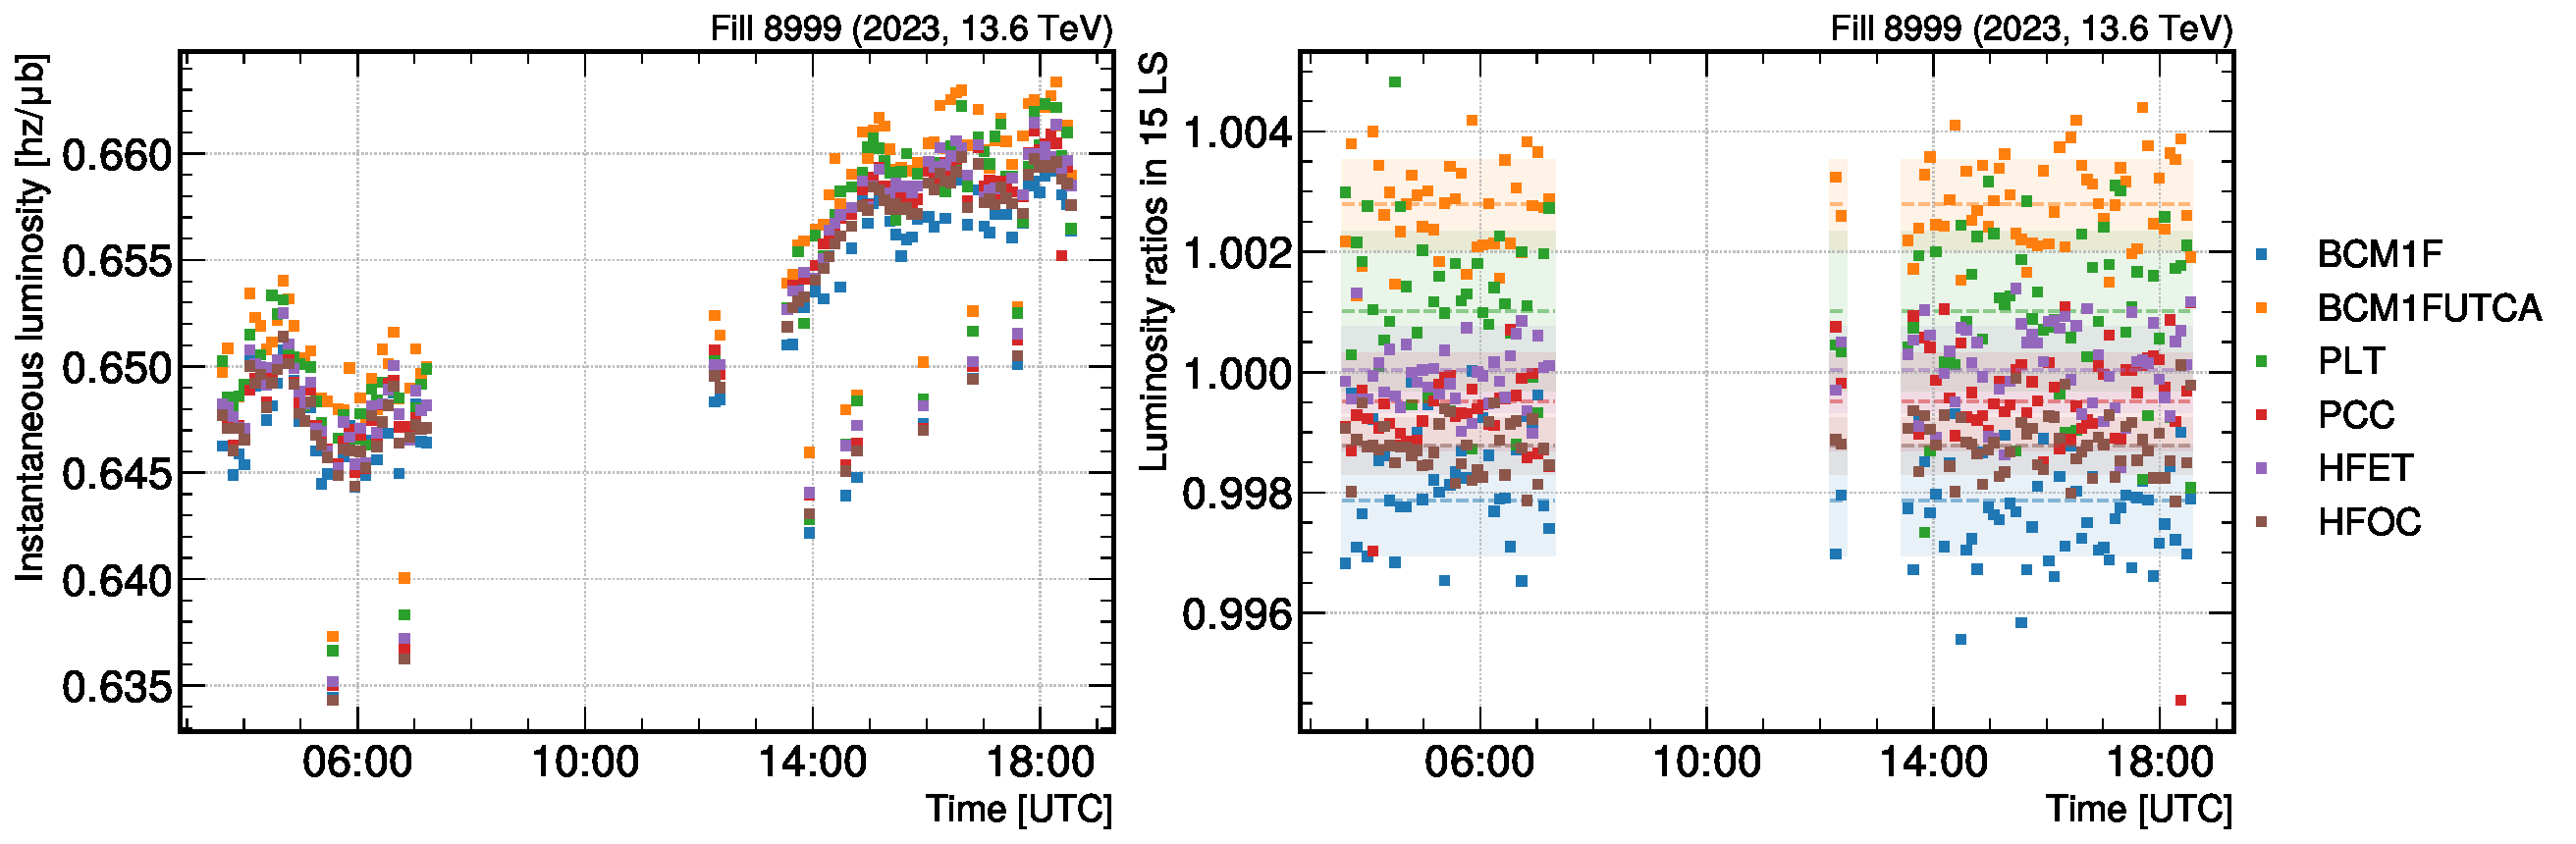
\includegraphics[width=0.7\paperwidth]{images/assets/vdm_head_on_lumi_vs_time_and_ratio.pdf}}
	\caption[Comparison of head-on luminosity measurements]{Head-on instantaneous luminosity measurements provided by the individual independently calibrated luminometers BCM1F, BCM1FUTCA, PLT, PCC, HFOC, and HFET during the LHC fill 8999 as a function of time.}
	\label{fig:vdm_head_on_lumi_vs_time_and_ratio}
\end{figure}

The data in \autoref{fig:vdm_head_on_lumi_vs_time_and_ratio} corresponds to the periods when the LHC beams were colliding head-on, with all six luminometers taking high-quality data, and for the sum of the nine BCIDs for which PCC data was recorded in zero bias events. Each point corresponds to a time window of 15 lumi sections (LS), with a lumi section spanning about 23 seconds. The ratio to the average measured luminosity is shown on the right and depicts an agreement well below 1\%. The statistical uncertainty associated with each point is found to be negligible and is not shown in the plot.

\begin{figure}[!htb]
	\centering
	\makebox[\textwidth]{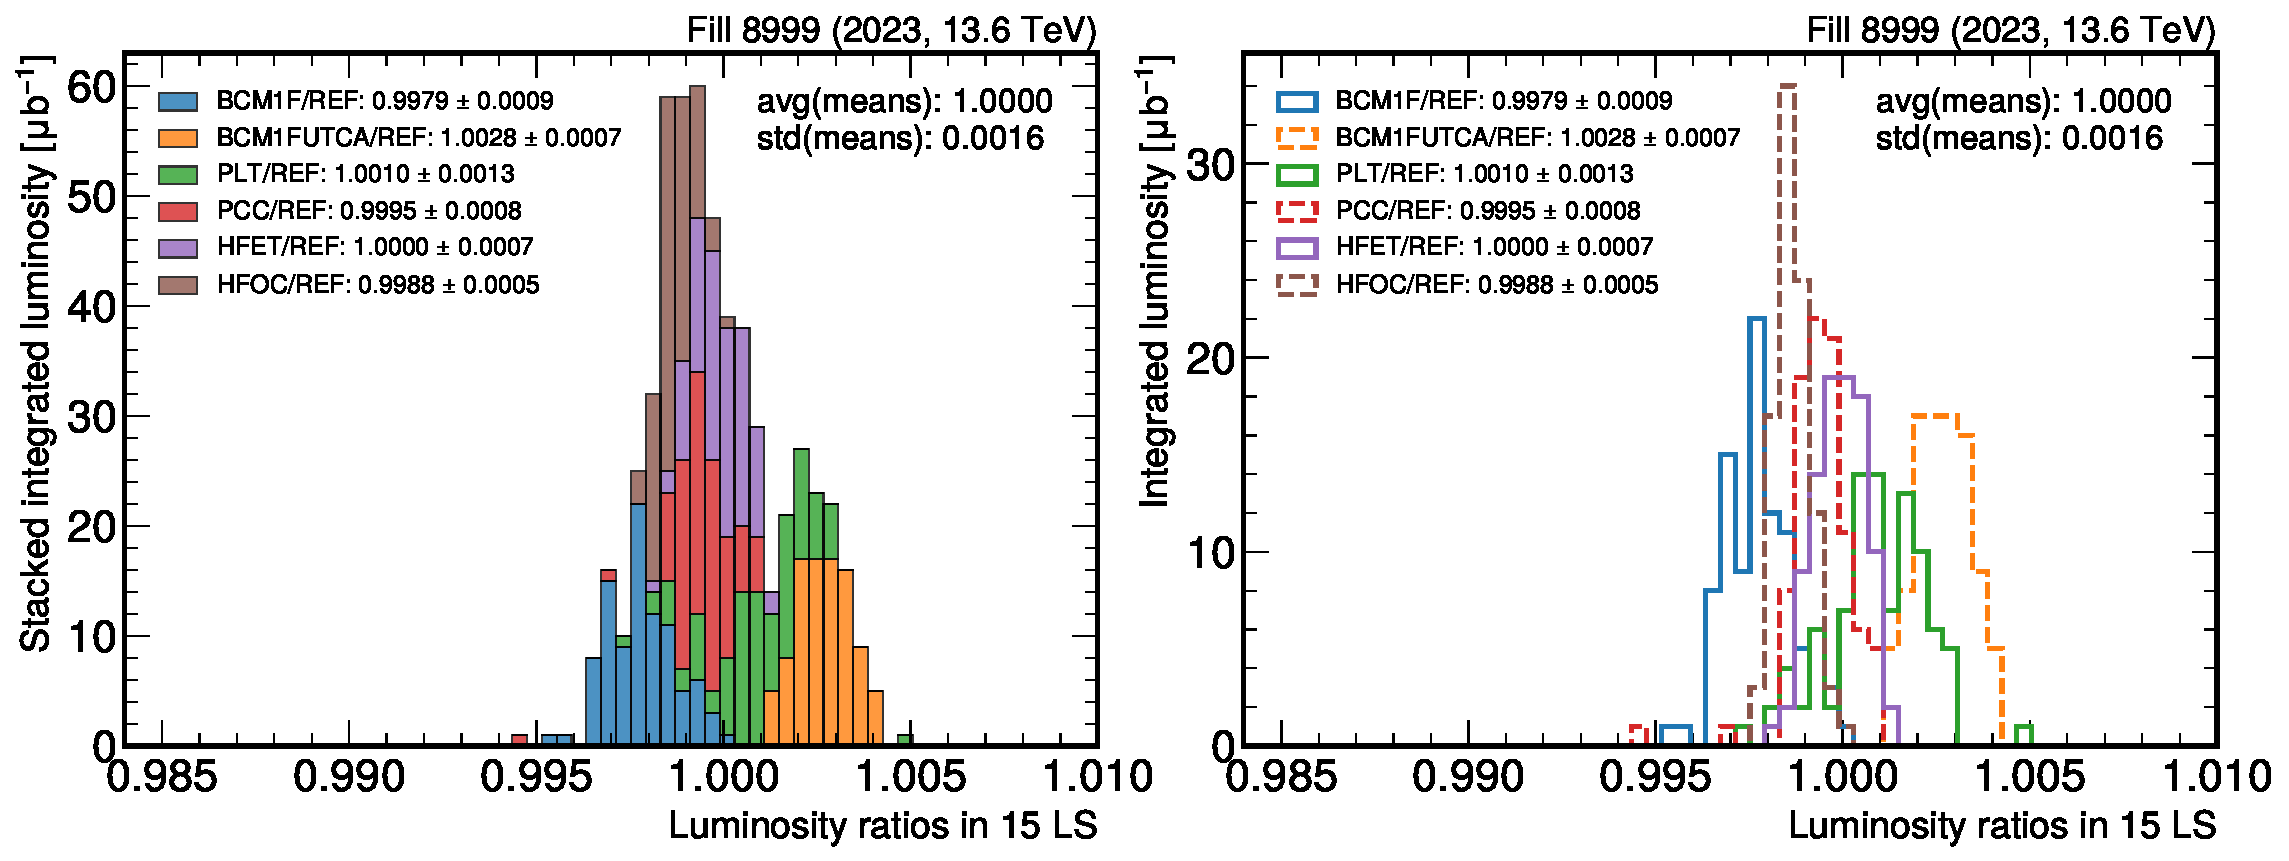
\includegraphics[width=0.7\paperwidth]{images/assets/vdm_ratio_histograms.pdf}}
	\caption[vdM luminosity ratio distributions]{Distributions of the ratio of the measured luminosities between different luminometers and the reference luminosity. The left plot shows a stacked distribution while the right plot shows individual distributions. The means and standard deviations of the individual distributions are shown. The reference luminosity (REF) corresponds to the average luminosity of all the individual luminometers.}
	\label{fig:vdm_ratio_histograms}
\end{figure}

With the vdM calibrations validated, they can be used to calibrate the rates of all luminometers for the entire running year in accordance with \autoref{eq:inst-luminosity}. The results of this calibration procedure are shown in \autoref{fig:vdm_only_year_stability}.

\begin{figure}[!htb]
	\centering
	\makebox[\textwidth]{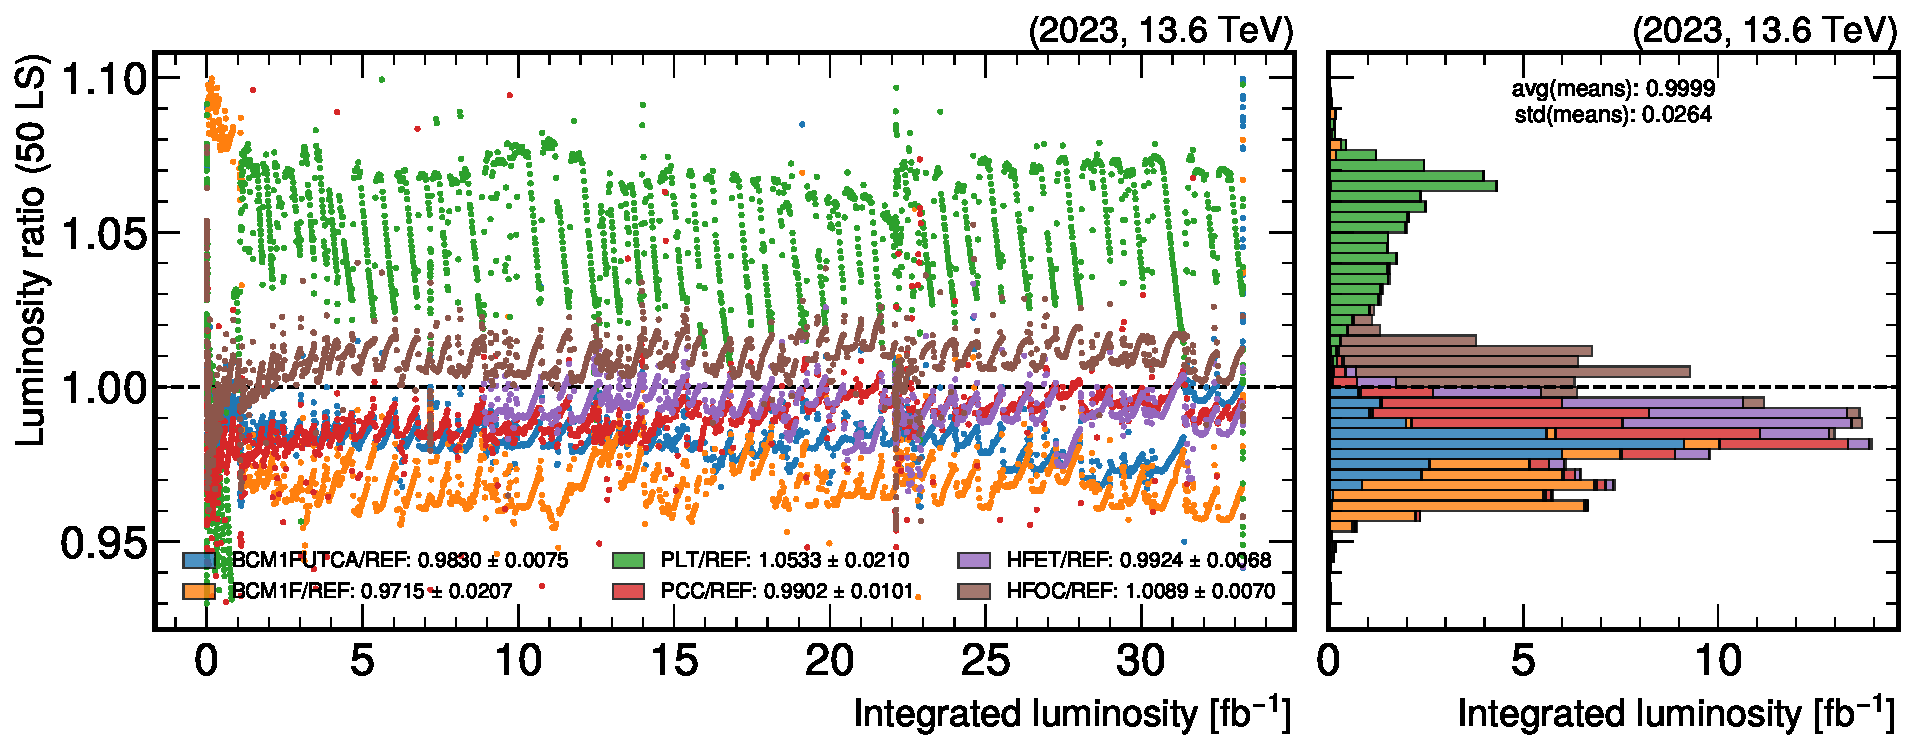
\includegraphics[width=0.7\paperwidth]{images/assets/vdm_only_year_stability.pdf}}
	\caption[Full year luminosity ratios with only vdM calibration]{The left plot shows the ratios of the luminosity measured in time windows of 50 LS (about 20 minutes) between the different luminometers and the average luminosity among them as a function of the integrated luminosity. The ratio distributions are shown in a histogram on the right, with the associated averages and standard deviations of the means indicated.}
	\label{fig:vdm_only_year_stability}
\end{figure}

Three main observations can be made when analyzing the ratios in \autoref{fig:vdm_only_year_stability}. The most obvious is the high discrepancy between different luminometers. PLT stands out as a clear example of this, but in general, the luminometers do not show good agreement. Secondly, some detectors exhibit significant steps throughout the year. Notable examples include BCM1F at the beginning and HFET from \(20.5 \, \text{fb}^{-1}\) to \(22 \, \text{fb}^{-1}\) and from \(27 \, \text{fb}^{-1}\) to \(27.5 \, \text{fb}^{-1}\). Lastly, the ratios show some non-linear responses, as is clearly seen in PLT. These observations highlight the difficulty in extrapolating the calibrations outside the vdM fill, as explained in \autoref{subsec:extrapolation_of_vdM_calibration}.

In the next sections, the issues of detector stability and non-linearity will be addressed, with examples of these corrections for the BCM1F and PLT detectors.

\subsection{Detector Stability}

The loss of efficiency that a detector exhibits throughout the year is corrected empirically by multiplying the detector's visible cross-section by a factor \(\epsilon\), as explained in \autoref{eq:luminosity_integration}. The method for obtaining these factors is detailed below.

Many fills conducted during the year 2023 had designated beam time to perform emittance scans. From these scans, the detectors' visible cross-sections are continuously measured, allowing for the tracking of the detectors' efficiency throughout the year. The loss of efficiency experienced by a detector is indicated by gradually decreasing \(\sigma_{\mathrm{vis}}\) measurements. When subsequent measurements do not follow the expected trend, it typically indicates that the detector is operating under non-optimized conditions. In such cases, the detector's running configurations are adjusted to restore normal operation conditions.

When extrapolating the VdM calibration to other fills, a linear regression is performed on the FOM values as a function of integrated luminosity. The fitted line is then normalized to the VdM since this represents our best calibration measurement. \autoref{fig:efficiency_bcm1f_example} shows the fit performed for the BCM1F measurements. The significant step at the beginning of \autoref{fig:efficiency_bcm1f_example} corresponds to a period when the BCM1F charge thresholds were set so high that it was counting noise as hits, leading to the apparent increase in efficiency.

\begin{figure}[!htb]
	\centering
	\makebox[\textwidth]{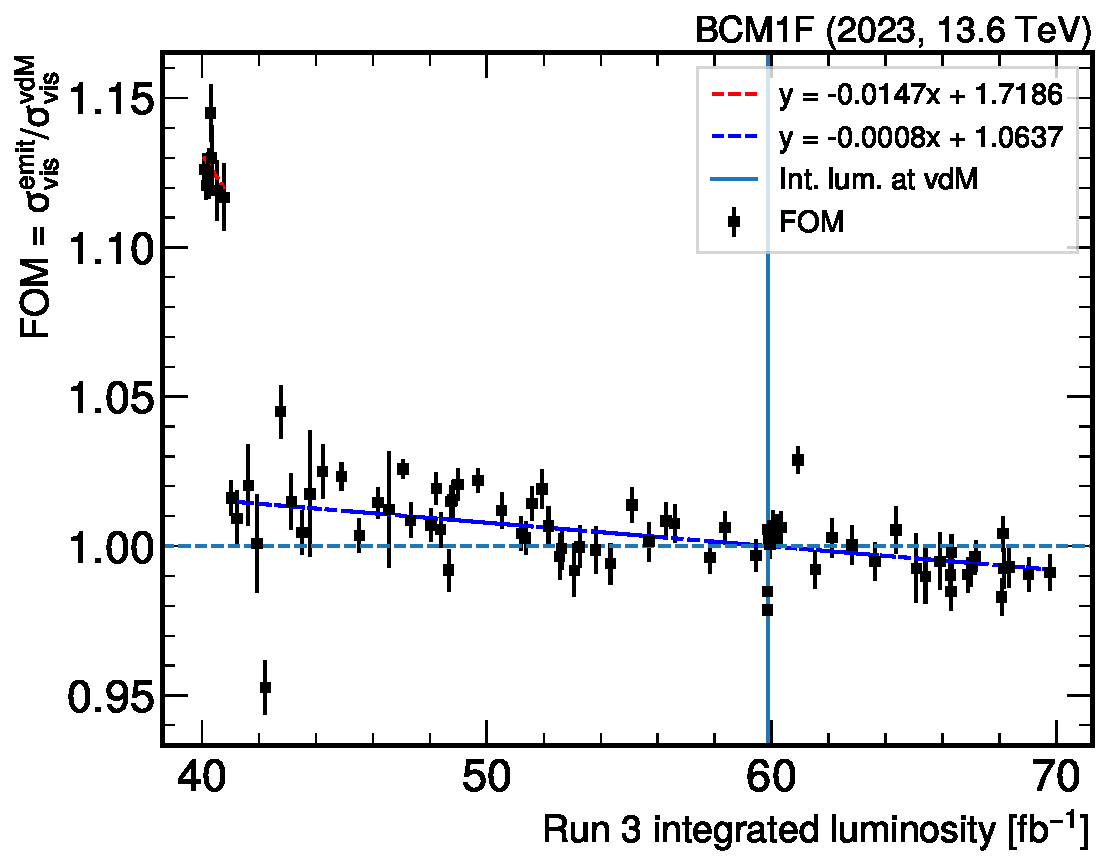
\includegraphics[width=0.5\paperwidth]{images/assets/efficiency_bcm1f_example.pdf}}
	\caption[BCM1F efficiency analysis results]{The results of emittance scan analysis for the BCM1F detector. The FOM values are shown as a function of Run 3 integrated luminosity. There are two distinct regions that are fitted independently, with the fit parameters shown in the legend.}
	\label{fig:efficiency_bcm1f_example}
\end{figure}

Once the fits are performed, the fit values at each point are used to extrapolate the VdM calibrations for the corresponding fills.

\subsection{Detector Non-Linearity}
\label{subsec:detector_non_linearity}

At the time of writting this thesis, only BCM1F and PLT were corrected for non-linearity. As explained in \autoref{subsec:extrapolation_of_vdM_calibration} a detector, assumed to have a good linear response to varying experimental conditions, is used as the reference for which other detectors will be corrected for. In this analysis the DT luminometer, referenced in autoref{subsec:dt}, will be used as the reference.

As in the previous section, this correction is also done at the fill level. However, in order to not strongly correlate the luminosity of the detectors to the reference detector, only a small number of fills, with a large SBIL range, are considerd. Let us consider this correction for PLT.

A total of 10 fills, spread across the year, were chosen for the slope extraction. For each fill, the luminosity ratios with respect to DT as a function of SBIL were computed. The fills before and after the vdM fill were placed in different groups since PLT's running configurations were changed in order to increase its efficiency for the vdM fill. The results of this analysis are shwon in \autoref{fig:plt_dt_relative_non_linearity}.

\begin{figure}[!htb]
	\centering
	\makebox[\textwidth]{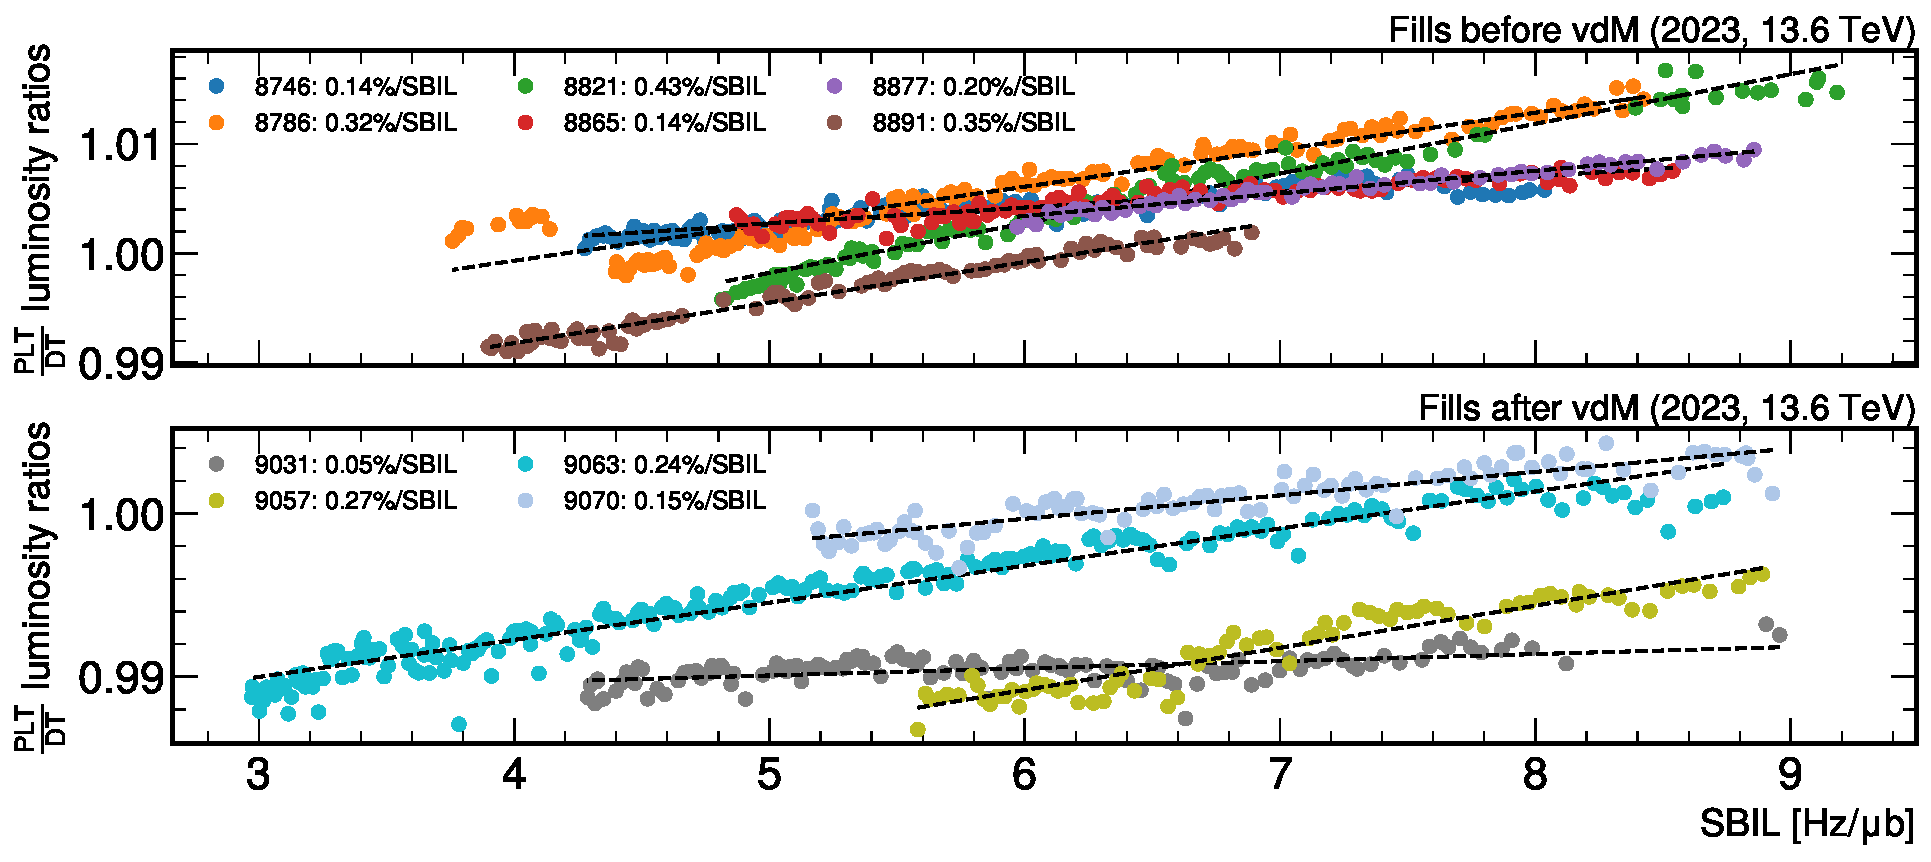
\includegraphics[width=0.7\paperwidth]{images/assets/plt_dt_relative_non_linearity.pdf}}
	\caption[PLT relative non-linearity slopes]{PLT non-linearity slopes extracted using DT as the reference luminometer for the 10 chosen fills. The dashed lines correspond to the linear fits and the slopes are shown in \% per SBIL in the legend. The slope values are added to the The upper plot contains the fills before the vdM program and the bottom plot contains the fills after.}
	\label{fig:plt_dt_relative_non_linearity}
\end{figure}

The extracted slopes have to by $0.8\%/\text{SBIL}$ since this was the non-linearity configuration assumed during online data taking. Averaging the 2 regions yielding $1.06\%/\text{SBIL}$ and $0.98\%/\text{SBIL}$ for before and after vdM, respectively. 

For BCM1F, the non-linearity was extracted from a $\mu$-scan fill. A $\mu$-scan is a much longer vdM scan that also spans a much wider SBIL range. The slopes were extracted in the same way as in the 2022 analysis \cite{CMS-PAS-LUM-22-001} and a $-0.12\%/\text{SBIL}$ correction was applied.

\subsection{Establishing a Reference Detector}

In \autoref{fig:vdm_only_year_stability} the ratios were taken with respect to the average luminosity of all luminometers. However, the luminosity results have to be available throught the brilcalc database constraints which places high constraints in the data format. For this reason, at the time of wrtting, DT was chosen as the reference detector. Since DT is not a independently calibrated luminometer due to lack of available statistics, it was calibrated to the average of the other luminometers, effectively representing the average luminosity among them.

During the 2023 analysis, DT had been cross-calibrated to HFET in fill 9036 which yielded an calibration of $\sigma^{\text{DT}}_{\mathrm{vis}} = 179725 \mu b$. To calibrate this cross-calibrate version of DT to the luminosity average the average ratio of every other luminometer with respect to this DT was taken. The results are shown in \autoref{tab:dt_cross_calibration}.

\begin{table}[!htb]
	\caption{Average and rms of all fully-corrected independently-calibrated luminometers with respect to HFET-cross-calibrated DT.}
	
	\label{tab:dt_cross_calibration}
	\centering
	\begin{tabular}{lcccc}
		\hline
		Luminometer & Average ratio to cross-calibrate DT & RMS \\
		\hline
		BCM1F     & 0.985 & 0.005 \\
		BCM1FUTCA & 0.985 & 0.005 \\
		HFET      & 0.998 & 0.005 \\
		HFOC      & 1.002 & 0.007 \\
		PLT       & 0.986 & 0.007 \\
		PCC       & 0.997 & 0.006 \\
		\hline
	\end{tabular}
\end{table}

Weighting the average of the values in \autoref{tab:dt_cross_calibration} by the inverse square of the individual rms yeilds a corrective factor of 0.991. This final cross-calibrated version of DT is used as a reference for the stability and non-linearity uncertainties discussed in the following section.

\section{Final Luminosity Results}

As in \autoref{subsec:vdm_consistency}, the year-long detector stability is illustrated. The best visible cross-sections are utilized, with stability and non-linearity corrections applied.

\begin{figure}[!htb]
    \centering
    \makebox[\textwidth]{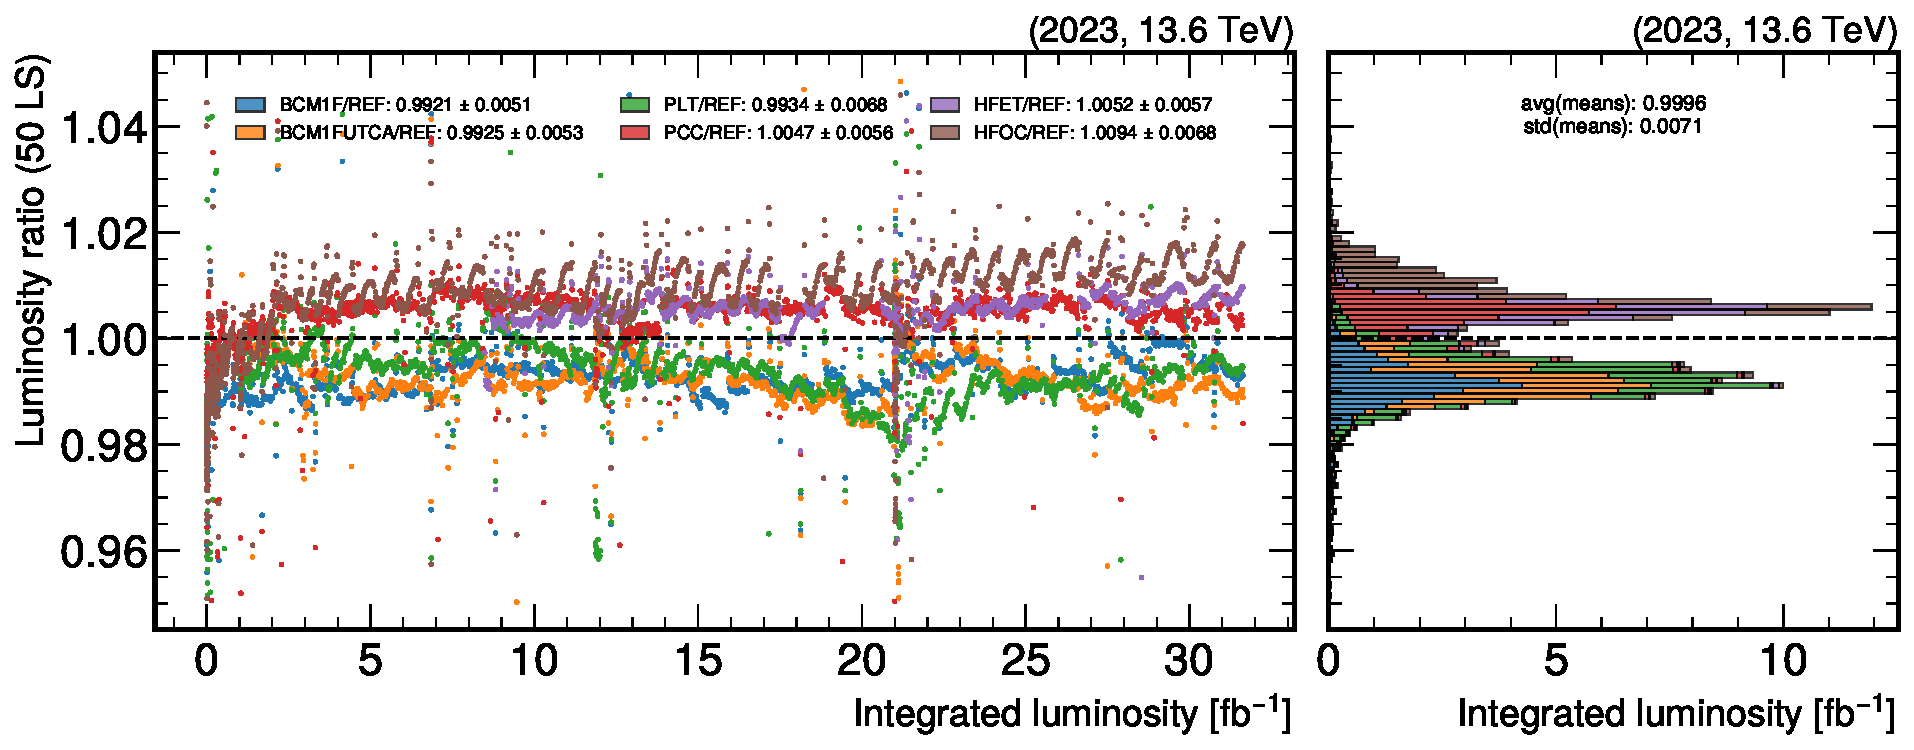
\includegraphics[width=0.7\paperwidth]{images/assets/final_preliminary_year_stability.pdf}}
    \caption[Final full year stability]{The left plot shows the ratios of the luminosity measured in time windows of 50 LS (about 20 minutes) between different luminometers and the reference luminometer as a function of the integrated luminosity over the 2023 pp data-taking period.}
    \label{fig:final_preliminary_year_stability}
\end{figure}

A comparison of \autoref{fig:vdm_only_year_stability} and \autoref{fig:final_preliminary_year_stability} reveals a significant improvement in detector agreement. The standard deviation of the means decreased from $2.6\%$ to $0.71\%$, indicating the uncertainty associated with the stability corrections.

\begin{figure}[!htb]
    \centering
    \makebox[\textwidth]{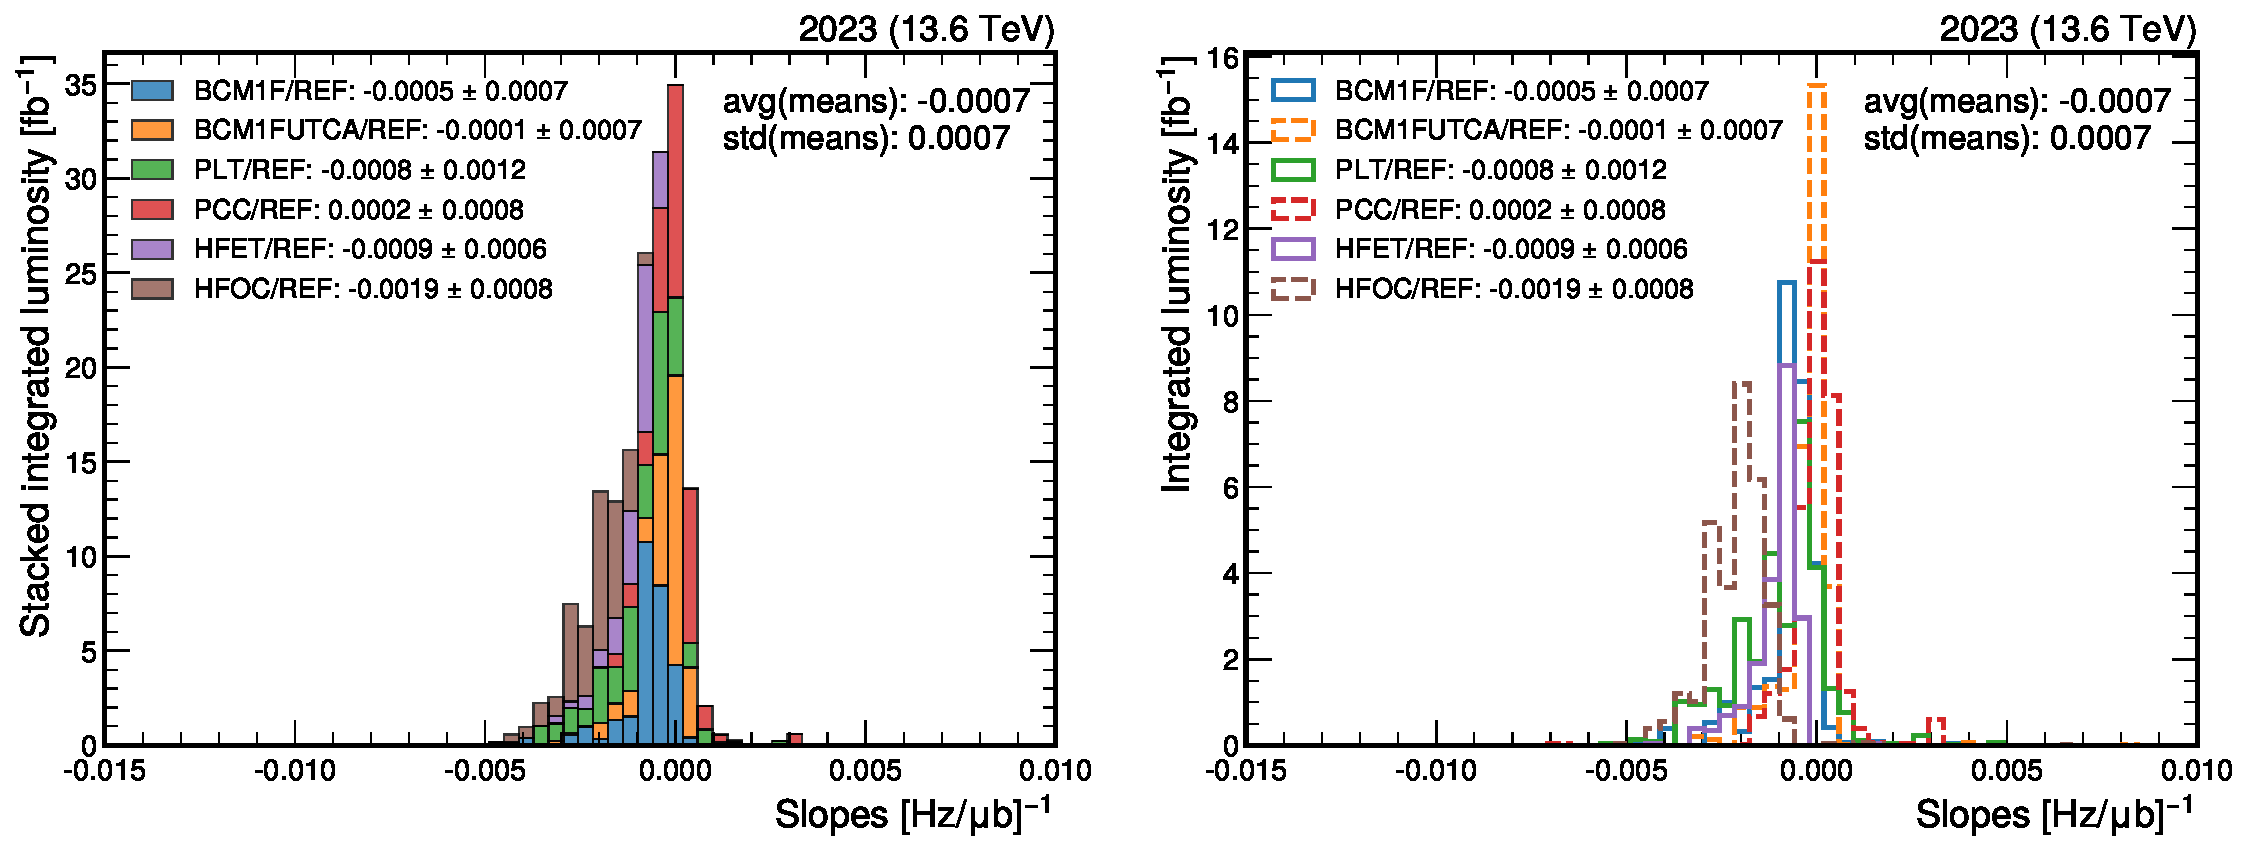
\includegraphics[width=0.7\paperwidth]{images/assets/year_slopes_final.pdf}}
    \caption[Residual relative non-linearity distributions]{Distributions of relative collinearity slope values between different luminometers and the DT luminometer taken as reference (REF). Each histogram entry is weighted by the integrated luminosity of the fill.}
    \label{fig:year_slopes_final}
\end{figure}

To assign an uncertainty to any residual non-linearity in the detectors, the slopes are extracted for all fills, as explained in \autoref
{subsec:detector_non_linearity}. The resulting distributions are analyzed, as shown in \autoref{fig:year_slopes_final}.

The detector with the maximum deviation, HFET, is chosen to assign the uncertainty for this step. HFOC is excluded due to its complex non-linearity effects which were not corrected and thus do not represent the current understanding. The value of $0.09\%/\text{SBIL}$ is multiplied by the average SBIL in 2023 of 6.6 H$z/\mu b$, resulting in an overall uncertainty of $0.59\%$.

Certain luminometers are unavailable for some periods throughout the year. Hence, all available luminometers are prioritized based on their measured luminosity contributions to the integrated luminosity. For this analysis, the priority order is DT, PCC, HFET, PLT, and BCM1FUTCA. The total delivered luminosity was 32.74 $\text{fb}^{-1}$, and the CMS recorded luminosity was 30.12 $\text{fb}^{-1}$, with an associated uncertainty of 1.28\%, as summarized in \autoref{tab:sum}.

\begin{table}[!h]
    \centering
    \caption{Summary of uncertainty contributions for the 2023 luminosity calibration analysis.}
    \label{tab:sum}
    \begin{tabular}{lc}
        \textbf{Source} & \textbf{Uncertainty} (\%) \\ \hline
        \textbf{Calibration} & \\
        Beam current & 0.20 \\
        Ghosts \& satellites & 0.10 \\
        Orbit drift & 0.02 \\
        Residual beam positions & 0.16 \\
        Beam-beam effects & 0.34 \\
        Length scale & 0.20 \\
        Factorization bias & 0.67 \\
        Scan-to-scan variation & 0.28 \\
        Bunch-to-bunch variation & 0.06 \\
        Cross-detector consistency & 0.16 \\ \hline
        \textbf{Integration} & \\
        Cross-detector stability & 0.71 \\
        Cross-detector linearity & 0.59 \\ % HFET
        \hline \hline
        Calibration & 0.89 \\
        Integration & 0.92 \\ % with HFET
        \hline
        Total & 1.28 \\
    \end{tabular}
\end{table}
